
\documentclass[lettersize,journal]{IEEEtran}
\usepackage{amsmath,amsfonts}
% \usepackage{algorithmic}
\usepackage{algcompatible}
\usepackage{algorithm}
% \usepackage[algo2e,ruled,linesnumbered]{algorithm2e}
\usepackage{array}
\usepackage[caption=false,font=normalsize,labelfont=sf,textfont=sf]{subfig}
\usepackage{textcomp}
\usepackage{stfloats}
\usepackage{url}
\usepackage{verbatim}
\usepackage{graphicx}
\usepackage{cite}
\hyphenation{op-tical net-works semi-conduc-tor IEEE-Xplore}
% updated with editorial comments 8/9/2021

\usepackage{csvsimple}
\usepackage{filecontents} 
\usepackage{tikz}
\usepackage{pdfplots}
\usepackage{amsthm}
\usepackage{amsmath,graphicx}
\usepackage{algorithm, algpseudocode}
\usepackage[utf8]{inputenc} % allow utf-8 input
\usepackage[T1]{fontenc}    % use 8-bit T1 fonts
\usepackage{hyperref}       % hyperlinks
\usepackage{url}            % simple URL typesetting
\usepackage{booktabs}       % professional-quality tables
\usepackage{amsfonts}       % blackboard math symbols  
\usepackage{bm}
\usepackage{nicefrac}       % compact symbols for 1/2, etc.
\usepackage{microtype}      % microtypography
\usepackage{xcolor}         % colors
\usepackage{tikz}
\usepackage{cite}
\usetikzlibrary{shapes}
\usetikzlibrary{shadows}
\usepackage{xspace}

% \renewcommand{\baselinestretch}{1.5}
\newcommand\strongconvparam[1]{\alpha^{(#1)}}
\newcommand\clusteropterr[1]{\delta^{(#1)}}
\newcommand{\wupdate}{\mathcal{WU}}
\newcommand{\zupdate}{\mathcal{ZU}}
\newcommand{\estmse}{{\rm MSE}}
\newcommand{\testmse}{\widehat{L} }
\newtheorem{assumption}{Assumption}
\newcommand{\scdots}[2][]{\mathinner{#1\overset{#2}{\cdots}#1}}
\definecolor{pinegreen}{cmyk}{0.92,0,0.59,0.25}
\definecolor{royalblue}{cmyk}{1,0.50,0,0}
\definecolor{lavander}{cmyk}{0,0.48,0,0}
\definecolor{violet}{cmyk}{0.79,0.88,0,0}
\tikzstyle{ncyan}=[circle, draw=cyan!70, thin, fill=white, scale=0.8, font=\fontsize{11}{0}\selectfont]
\tikzstyle{ngreen}=[circle,  draw=green!70, thin, fill=white, scale=0.8, font=\fontsize{11}{0}\selectfont]
\tikzstyle{nred}=[circle, draw=red!70, thin, fill=white, scale=0.8, font=\fontsize{11}{0}\selectfont]
\tikzstyle{ngray}=[circle, draw=gray!70, thin, fill=white, scale=0.55, font=\fontsize{14}{0}\selectfont]
\tikzstyle{nyellow}=[circle, draw=yellow!70, thin, fill=white, scale=0.55, font=\fontsize{14}{0}\selectfont]
\tikzstyle{norange}=[circle,  draw=orange!70, thin, fill=white, scale=0.55, font=\fontsize{10}{0}\selectfont]
\tikzstyle{npurple}=[circle,draw=purple!70, thin, fill=white, scale=0.55, font=\fontsize{10}{0}\selectfont]
\tikzstyle{nblue}=[circle, draw=blue!70, thin, fill=white, scale=0.55, font=\fontsize{10}{0}\selectfont]
\tikzstyle{nteal}=[circle,draw=teal!70, thin, fill=white, scale=0.55, font=\fontsize{10}{0}\selectfont]
\tikzstyle{nviolet}=[circle, draw=violet!70, thin, fill=white, scale=0.55, font=\fontsize{10}{0}\selectfont]
\tikzstyle{qgre}=[rectangle, draw, thin,fill=green!20, scale=0.8]
\tikzstyle{rpath}=[ultra thick, red, opacity=0.4]
\tikzstyle{legend_isps}=[rectangle, rounded corners, thin,fill=gray!20, text=blue, draw]
\usetikzlibrary{positioning}
\newtheorem{proposition}{Proposition}%[section]
\newtheorem{theorem}{Theorem}%[section]
\newtheorem{definition}[theorem]{Definition}
\newtheorem{lemma}[theorem]{Lemma}
\newtheorem{example}[theorem]{Example}
\newtheorem{corollary}[theorem]{Corollary}

\input{mlbpbook_macros}
\newcommand{\graphmnist}{\graph^{(\rm MNIST)}}
\newcommand{\nodesmnist}{\nodes^{(\rm MNIST)}}
\newcommand{\edgesmnist}{\edges^{(\rm MNIST)}}
\newcommand{\pdgap}[1]{{\rm gap}_{#1}} 
\newcommand{\localvalsetsize}[1]{m^{(\rm val)}_{#1}} 
\newcommand{\localtrainsetsize}[1]{m^{(\rm train)}_{#1}} 

\begin{document}

\title{Networked Federated Learning}
%
%
% author names and IEEE memberships
% note positions of commas and nonbreaking spaces ( ~ ) LaTeX will not break
% a structure at a ~ so this keeps an author's name from being broken across
% two lines.
% use \thanks{} to gain access to the first footnote area
% a separate \thanks must be used for each paragraph as LaTeX2e's \thanks
% was not built to handle multiple paragraphs
%

\author{Yasmin~SarcheshmehPour, Yu Tian, Linli Zhang and Alexander Jung% <-this % stops a space
	\thanks{}% <-this % stops a space
	\thanks{}% <-this % stops a space
}



\maketitle

\markboth{Some Journal}%
{Shell \MakeLowercase{\textit{et al.}}: Bare Demo of IEEEtran.cls for IEEE Journals}


\begin{abstract}
We develop the theory and algorithmic toolbox for networked federated learning in 
decentralized collections of local datasets with an intrinsic network structure. This 
network structure arises from domain-specific notions of similarity between local datasets. 
Different notions of similarity are induced by spatio-temporal proximity, statistical 
dependencies or functional relations. Our main conceptual contribution is to formulate 
networked federated learning using a generalized total variation minimization. This 
formulation unifies and considerably extends existing federated multi-task learning 
methods. It is highly flexible and can be combined with a broad range of parametric 
models including Lasso or deep neural networks. Our main algorithmic contribution 
is a novel networked federated  learning algorithm which is well suited for distributed computing 
environments such as edge computing over wireless networks. This algorithm is robust 
against inexact computations arising from limited computational resources including processing 
time or bandwidth. For local models resulting in convex problems, we derive precise conditions 
on the local models and their network structure such that our algorithm learns nearly optimal 
local models. Our analysis reveals an interesting interplay between the convex 
geometry of local models and the (cluster-) geometry of their network structure. 
\end{abstract}


\begin{IEEEkeywords}
	federated learning, clustering, complex networks, total variation, regularization
\end{IEEEkeywords}

% For peer review papers, you can put extra information on the cover
% page as needed:
% \ifCLASSOPTIONpeerreview
% \begin{center} \bfseries EDICS Category: 3-BBND \end{center}
% \fi
%
% For peerreview papers, this IEEEtran command inserts a page break and
% creates the second title. It will be ignored for other modes.


\section{Introduction}
\label{sec:intro}

Many important application domains generate collections of local datasets that are related via 
an intrinsic network structure \cite{BigDataNetworksBook}. Two timely application domains 
generating such networked data are (i) the high-precision management of pandemics and (ii) the Internet of Things (IoT) \cite{Wollschlaeger2017}.
% \cite{Wollschlaeger2017,Satyanarayanan2017}
Such local datasets are generated by smartphones, wearables or industrial IoT devices \cite{Ates:2021ug}.
% \cite{Ates:2021ug,BOYES20181}
These local datasets are related via physical contact networks, social networks \cite{NewmannBook}, 
co-morbidity networks \cite{NetMedNat2010}, or communication networks \cite{Grantz:2020wn}. 

Federated learning (FL) is an umbrella term for machine learning (ML) techniques that collaboratively 
train models on decentralized collections of local datasets \cite{pmlr-v54-mcmahan17a,Cheng2020,Smith2017}. 
These methods carry out computations such as gradient descent steps during model training at the location 
of data generation, rather than first collecting all data at a central location \cite{ShipCompute}. 
FL methods are appealing for applications involving sensitive data (such as healthcare) as they 
do not require the exchange of raw data but only model (parameter) updates without leaking sensitive information in local datasets \cite{Cheng2020}. 
% By sharing only model updates, FL methods are considered privacy-friendly in the sense of not leaking  sensitive information in local datasets \cite{DiffPrivADMM}.
Moreover, FL methods can offer robustness 
against malicious data perturbation due to its intrinsic averaging or aggregation over large collections 
of (mostly benign) datasets \cite{Sattler2020}.

FL applications often face local datasets with different statistical properties \cite{Ghosh2020}. 
Each local dataset induces a separate learning task that consists of learning (or optimizing) 
the parameters of a local model. This paper studies an optimization method to train local models 
that are tailored (or ``personalized'') to the statistical properties of the corresponding local dataset. This method 
is an instance of regularized empirical risk minimization (or structural risk minimization). In particular, it 
uses a measure (see Section \ref{sec_nLasso}) for the variation of local model parameters as regularizer term. We 
solve the resulting optimization (or learning) problem using a primal-dual method that can be implemented 
as message passing over the network structure of local datasets (see Section \ref{sec_federatedml}). 

Clustered FL addresses the heterogeneity of local datasets using various forms of a clustering 
assumption \cite{NIPS2008_fccb3cdc,Ghosh2020,SemiSupervisedBook}. Informally, our clustering 
assumption requires local datasets and their associated learning tasks to form a few disjoint
subsets or clusters. As a result, local datasets belonging to the same cluster have similar 
statistical properties and, in turn, similar optimal parameter values for the corresponding local models. 
Section \ref{sec:format} makes this clustering assumption precise via Assumption \ref{asspt_weights_clustered}. 
The main contribution of this paper is a detailed characterization of the cluster structure and local model 
geometry for local datasets that allow our methods to pool local datasets that form statistically 
homogeneous clusters of datasets (see Section \ref{sec_when_does_it_work}).

What sets our approach apart from existing methods for clustered FL \cite{Ghosh2020,NIPS2008_fccb3cdc} 
is that we exploit known pairwise similarities between local datasets. These similarities are encoded by 
the weighted undirected edges of an \emph{empirical graph} \cite{SemiSupervisedBook}. 
% {\color{red} Networked FL (NFL) uses the empirical graph of networked data to cluster (or pool) local datasets into nearly homogenous (``i.i.d.'') training sets. }
% {\color{red} Each resulting cluster of local datasets is then used to train a cluster-specific model which is common for all local datasets in the same cluster. }
Instead of a trivial combination of clustering methods and cluster-wise model training, 
our NFL method (see Algorithm \ref{alg1}) interweaves the pooling of local datasets with 
model training. We use the connectivity of the empirical graph to guide this pooling (see Section \ref{sec_federatedml}).

We can interpret NFL methods as enhanced graph clustering methods that combine the graph structure 
with the statistical properties of local datasets to cluster the nodes of the empirical graph \cite{Luxburg2007}. 
Another related interpretation of NFL is that of a special form of multi-task learning. Indeed, each cluster of local 
datasets gives rise to a separate learning task (finding optimal parameters for all cluster nodes) \cite{NIPS2008_fccb3cdc}. 
Yet another interpretation of NFL, that will be revealed in Section \ref{sec_nLasso}, is that of network (flow) optimization \cite{BertsekasNetworkOpt,RockNetworks}.

Let us emphasize that our approach requires a useful choice for the empirical graph of networked data. 
The connectivity of nodes (that represent local datasets) in the empirical graph must reflect 
the clustering of local datasets sharing similar statistical properties. Some application domains 
offer a natural choice for the empirical graph, e.g., based on physical models, functional relations, 
or the computing infrastructure \cite{NewmannBook}. 

If a natural choice for the empirical graph is not available, we can use principled statistical tests 
for the similarity between two datasets \cite{CSGraphSelJournal}. We demonstrate some of these 
methods in the numerical experiments of Section \ref{sec_numexp}. However, graph learning is beyond 
the scope of this paper (see Section \ref{sec_conclusion}). 

\vspace*{-3mm}
\subsection{Related Work}

Similar to \cite{NetworkLasso,LocalizedLinReg2019,Smith2017,Nassif2020,Xu2011}, 
we use regularized empirical risk minimization (RERM) to learn tailored models for local datasets. 
For each local dataset we obtain a separate learning task that amounts to finding 
an (approximately) optimal choice for the parameters of a local model. These individual 
learning tasks are coupled via the undirected weighted edges of an empirical graph (see Section \ref{sec:format}). 
In contrast to \cite{Xu2011}, which uses a probabilistic model for the empirical graph, 
we consider the empirical graph as fixed and known (non-random). 

To capture intrinsic cluster structure of networked data, we use a generalized total 
variation (GTV) of the 
model parameters as the regularizer. GTV unifies and extends several existing notions 
of total variation \cite{NetworkLasso,LocalizedLinReg2019,Smith2017,Nassif2020}. 
GTV is parametrized by a penalty function which is used to measure the difference of local model 
parameters at neighbouring nodes in the empirical graph. Computationally, the main restriction for 
the choice of penalty function is that it must allow for efficient computation of the corresponding proximity  
operator \eqref{equ_def_proximity_operator}. Some authors refer to such functions as ``proximable'' \cite{Condat2013}. 

%For GTV penalty functions being a norm and local loss functions being smooth and convex, 
%we upper bound the deviation between solutions of GTV minimization and an oracle-based 
%approach that serves as an (impractical) benchmark. This benchmark is obtained by assuming 
%perfect knowledge about the cluster structure of the empirical graph (see Assumption \ref{asspt_weights_clustered}). 

Our analysis reveals conditions on the network structure between local datasets and their 
local models such that GTV minimization is able to identify the cluster structure of the empirical graph. 
This is relevant for the application of GTV minimization to clustered FL \cite{NIPS2008_fccb3cdc,Ghosh2020}. 
In contrast to existing work on clustered FL, we exploit a known similarity structure between local 
datasets. We represent these similarities by the edges of an empirical graph. 

%This analysis restricts the loss functions, used to score local model parameters, to be smooth 
%and convex functions of the local model parameters (see Assumption \ref{asspt_FIM_lower_bound}). 
%However, our NFL method can also be applied to non-convex and non-smooth loss functions as long 
%as they admit an efficient evaluation of their proximity operators.  

%Using different instances of GTV, obtained from different choices for the penalty function, as a regularizer 
%results in different formulations of FL as RERM. We will refer to this family of RERM instances as GTV minimization. 
GTV minimization unifies and considerably extends well-known optimization models for FL 
including the TV minimization and network Lasso (nLasso) \cite{NetworkLasso,LocalizedLinReg2019,Smith2017,Nassif2020}. 
GTV is an instance of the non-quadratic regularizer put forward in \cite{Nassif2020}. 
In contrast to \cite{Nassif2020}, which uses a combination of gradient descent and distributed averaging 
methods, we use a primal-dual method to solve the resulting GTV minimization. We provide precise 
conditions such that GTV minimization captures the inherent cluster structure of networked data. 

The methods in \cite{LocalizedLinReg2019} 
are limited to generalized linear models. In contrast, we consider GTV minimization methods that can be combined 
with a wide range of (potentially non-linear) parametrized models including graphical Lasso or deep neural networks \cite{HastieWainwrightBook,Goodfellow-et-al-2016}. 
% {\color{red} We emphasize that our analysis of GTV minimization (see Section \ref{sec_when_does_it_work}) only applies if it is combined with local models resulting in a convex loss function. However, in principle our NFL algorithm can be combined with any parametric local model that can be trained efficiently. Examples for such local models include generalized linear models and artificial neural networks which can be trained using stochastic gradient descent methods \cite{Goodfellow-et-al-2016}. }

A substantial body of work studies computational aspects of GTV minimization \cite{NIPS2008_fccb3cdc}. 
Efficient algorithms for GTV minimization have been proposed for relevant computational infrastructures 
such as wireless networks of low-complexity devices \cite{DistrOptStatistLearningADMM,NedicTransAC2009}. We would like to highlight the recent study \cite{NEURIPS2018_8fb21ee7} 
of intrinsic computational complexity and efficient primal-dual methods for GTV minimization. While 
\cite{NEURIPS2018_8fb21ee7} only uses the network diameter, our analysis involves more fine-grained properties of empirical graph. 

Similar to \cite{NEURIPS2018_8fb21ee7}, our algorithmic approach to FL is based on an established primal-dual 
method for optimization \cite{pock_chambolle_2016}. This primal-dual method is 
appealing for FL application in several aspects. First, as we show in Section \ref{sec_federatedml}, the primal-dual 
method \cite[Alg. 6]{pock_chambolle_2016} can be implemented as a message passing protocol over the empirical graph. 
Message passing algorithms are scalable to massive collections of local datasets as long as their empirical graph 
is sparse (e.g., a bounded degree network) \cite{Yedidia:2011aa}. 

The primal-dual method\cite[Alg. 6]{pock_chambolle_2016} also offers robustness against limited computational 
resources and imperfections. One example for such imperfections are inexact evaluations of proximity 
operators. Evaluating the proximity operator \eqref{equ_def_proximity_operator} is to solve an optimization 
problem, e.g., using iterative methods such as gradient descent  \cite{Condat2013,ChambolleStochPDHG2018}.
Indeed, each iteration of the primal-dual method requires to update local model parameters by 
solving a separate model training problem for each local dataset. Given finite computational resources, 
these local model updates can only be solved up to some non-zero optimization error. 
The effect of inexact updates in primal-dual methods has been analyzed recently \cite{Rasch:2020tx}. 

In contrast to its computational aspects, the statistical aspects of GTV minimization are far less 
understood \cite{NetworkLasso,Smith2017}. Our main focus is on the dependency of solutions to 
GTV minimization on the cluster structure of networked data. It is possible to frame GTV 
minimization as the learning or recovery of group-sparse models \cite{BuhlGeerBook}. 
However, it is unclear how the group-sparse models underlying GTV minimization are related to the 
fine-grained properties (such as cluster structure) of the empirical graph.  

The closest to our work is the recent analysis of convex clustering \cite{JMLR:v22:18-694}. As convex 
clustering is a special case of GTV minimization (see Section \ref{sec_interpreations}), our work 
significantly extends the results in \cite{JMLR:v22:18-694}. Moreover, in contrast to \cite{JMLR:v22:18-694}, 
we characterize the cluster structure of local datasets using network flows.  

%Existing methods for clustered FL do not exploit the presence of a known network structure. In contrast, we 
%use the network structure between local datasets to guide their grouping into (statistically) homogenous clusters. 
%We provide a precise characterization of the data network structure and the amount of available data such that 
%GTV minimization is able to recover the true underlying cluster structure (see Section \ref{equ_analysis_error}). 
%This characterization is in the form of an upper bound on the deviation between the solution of GTV minimization 
%and an oracle FL method that is provided with the (in practice unknown) partition of local datasets into clusters. 



%our 
%algorithm only requires access to the local datasets on a sufficiently large subset of nodes. 



\subsection{Contribution} 
%We propose and study a novel family of FL algorithms that learn separate (tailored or personalized) 
%model parameters for each local dataset within a collection of networked data. These algorithms  networked data is 
%represented 
%by a given undirected empirical graph whose edges connect (statistically) similar datasets. 
%Our method exploits the cluster structure of the empirical graph to adaptively pool datapoints 
%for learning model weights. 

%This paper unifies and extends recent approaches to localized linear regression and classification \cite{}. 
We next enumerate the main contributions of this paper. 
\begin{itemize} 
\item We propose and study GTV minimization as an optimization model for NFL. GTV minimization 
is an instance of RERM using the variation of local model parameters as a regularizer. GTV minimization 
unifies and extends existing optimization models for FL, including nLasso and MOCHA \cite{Smith2017}. 
It is flexible as it can be combined with a range of parametrized local models. The main 
restriction is that local models must be parametrized by a common finite-dimensional 
Euclidean space $\mathbb{R}^{\dimlocalmodel}$. 
%Our setting covers many important ML 
%methods such as (regularized) generalized linear models. However, it does not cover 
%non-parametric local models such as decision trees. 

\item We explore the duality between GTV minimization and network flow optimization \cite{BertsekasNetworkOpt}. 
This duality is a generalization of some well-known duality results for network optimization \cite{RockNetworks}. 
% {\color{red} In particular, GTV minimization generalizes the optimal differential problem of \cite{RockNetworks} to vector-valued node values, which represent local model parameters.} 
The dual of GTV minimization generalizes the minimum cost flow 
problem of \cite{BertsekasNetworkOpt} to vector-valued flows. 

% formulate multi-task learning in heterogeneous (non-i.i.d.) data as a special case of a network Lasso problem. 
\item Our main methodological contribution is a novel family of NFL algorithms (see Algorithm \ref{alg1}). 
This family is obtained by solving different instances of GTV minimization with an established primal-dual method for structured optimization \cite{Condat2013}. 
% {\color{red} This family is parametrized by design choices for the local models and a penalty function used to measure the GTV of model parameters. }
Algorithm \ref{alg1} alternates between separate local model parameter updates that are regularized by previously
received model parameters and sharing these updates between 
neighbouring nodes (see Section \ref{sec_federatedml}).
% The local model parameter updates are regularized by previously received model parameter updates from neighbouring nodes. 
The computational complexity of the algorithm is essentially the same as the computational complexity of training the local models separately 
% {\color{red}(which corresponds to networked data with a trivial empirical graph without any edges)}. 
Algorithm \ref{alg1} can be combined with a wide range of 
parametric ML models and notions of TV (obtained for different GTV penalty functions). The main requirement 
is merely the existence of an efficient training method for 
the local models. The choice for the GTV penalty function is only restricted by requiring an efficient 
way to compute its convex conjugate. 
%By exploiting the network structure of data, our algorithm can also handle partially 
%observed datasets which is relevant for semi-supervised learning settings. %and can be implemented as scalable message passing protocols that are robust against modelling errors and . 
% be approximately constant over 
\item Our main analytical contribution is an upper bound on the estimation error incurred by GTV minimization. 
This upper bound reveals sufficient conditions on the local datasets and network structure such 
that our method achieves the performance of an oracle-based method that perfectly knows the true  
cluster structure of the data network. We emphasize that our analysis only applies to GTV minimization 
(i) using a penalty function being a norm (ii) and local models characterized by smooth and convex loss functions. 
Thus, our bounds do not apply to methods that either use graph Laplacian quadratic form 
as regularizer (such as MOCHA) or local models resulting in non-convex loss functions (deep nets). 
However, our analysis might provide also insight into the statistical properties of GTV minimization for 
non-convex local models (i.e., resulting in non-convex loss functions). 
%For example, we might locally approximate the non-convex loss functions of a deep net using 
%a smooth and convex (quadratic) surrogate function. 
\end{itemize}

\subsection{Outline} 
Section \ref{sec:format} introduces the concept of an empirical graph to represent collections of local 
datasets, the corresponding local models as well as their similarity structure. 
% The nodes of the empirical graph not only carry the local datasets but also the parameter vector of a local model that is tailored (or ``personalized'') to the corresponding local dataset. 
Section \ref{sec_nLasso} 
introduces GTV as a measure for the variation of local model parameters across the edges in 
the empirical graph. As discussed in Section \ref{sec_primal_problem}, GTV minimization balances  
the variation of local model parameters over well-connected local datasets (forming a cluster) and incurring 
a small loss (training error) for each local dataset. The dual problem to GTV minimization is then 
explained in Section \ref{sec_dual_problem_GTV_Min}. Section \ref{sec_interpreations} presents several 
useful interpretations of GTV minimization and its dual. 
Section \ref{sec_federatedml} applies a well-known primal-dual optimization method 
to solve GTV minimization and its dual in a fully distributed fashion via message passing over the empirical graph (see Algorithm \ref{alg1}). 
% The resulting NFL method (see Algorithm \ref{alg1}) learns the local model parameters in a fully distributed fashion via message passing over the empirical graph. 
The results of numerical experiments are discussed in Section \ref{sec_numexp}. 

\subsection{Notation} %We denote matrices and vectors using boldface upper and lower case letters.
The identity matrix of size $n\!\times\!n$ is denoted $\mathbf{I}_{n}$, with the subscript omitted
if the size $n$ is clear from context. We use $\| \cdot \|$ to denote some norm defined on the Euclidean 
space $\mathbb{R}^{\dimlocalmodel}$ and $\| \cdot \|_{*}$ to denote its dual norm \cite[Appx. 1.6.]{BoydConvexBook}. 
%The positive part of a real number $a\!\in\!\mathbb{R}$ is $(a)_{+} \!=\! \max\{a, 0\}$.
Two important examples are the Euclidean norm $\| \vw \|_{2} \!\defeq\!\sqrt{\sum_{\featureidx=1}^{\dimlocalmodel} w_{\featureidx}^{2}}$ and 
the $\ell_{1}$ norm $\| \vw \|_{1} \!\defeq\!\sum_{\featureidx=1}^{\dimlocalmodel} |w_{\featureidx}|$ of a vector $\vw \!= \!(w_{1},\ldots,w_{\dimlocalmodel})^{T} \in \mathbb{R}^{\dimlocalmodel}$ . 
% Given a positive semi-definite matrix $\mM$, we define the norm $\| \vw \|_{\mM} \defeq \sqrt{ \vw^{T} \mM \vw}$. 
It will be convenient to use the notation $(1/2\tau)$ instead of $(1/(2\tau))$. %For a positive definite matrix $\mathbf{C}$,
%we define the induced norm $\| \vx \|_{\mathbf{C}} \defeq \sqrt{ \vx^{T} \mathbf{C} \vx }$.
We will need the (vector-wise) clipping operator
\vspace{-2mm}
\begin{equation} 
\vspace{-2mm}
	\label{equ_vector_clipping}
	\mathcal{T}^{(\gamma)}(\vw)\!\defeq\! \begin{cases} \gamma \vw/\|\vw\|_{2} & \mbox{ for } \| \vw \|_{2} \!\geq\!\gamma \\
		\vw  & \mbox{ otherwise.} \end{cases} 
\end{equation} 
The scalar clipping operator $\mathcal{T}^{(\gamma)}(w)$ is obtained as a special case of \eqref{equ_vector_clipping} 
by considering the scalar $w$ as a vector with a single entry (where $\normgeneric{\mathbf{w}}{2} = |w|$). 
Given a closed proper convex function $f(\vx)$ with domain being a subset of $\mathbb{R}^{\dimlocalmodel}$, 
we define its associated convex conjugate function as \cite{BoydConvexBook}
\begin{equation} 
\label{equ_def_conv_conj}
f^{*} (\vx) \defeq \sup\limits_{\vz \in \mathbb{R}^{\dimlocalmodel}}  \vx^{T} \vz - f(\vz). 
\vspace{-2mm}
\end{equation} 
We will use the proximity operator of a closed proper convex function $f(\vx)$, 
defined as \cite{DistrOptStatistLearningADMM} 
\begin{equation}
\label{equ_def_proximity_operator}
\proximityop{f}{\vx}{\rho}\!\defeq\!\argmin_{\vx'} f(\vx')\!+\!(\rho/2) \| \vx - \vx'\|^{2}_{2} \mbox{ with } \rho\!>\!0.
\end{equation} 
Note that the minimum in \eqref{equ_def_proximity_operator} exists and is unique since the objective 
function is strongly convex \cite{BoydConvexBook}. 


\section{Problem Formulation}
\label{sec:format}


%????Figure \ref{fig_local_dataset} illustrated an weighted undirected ``empirical'' graph $\graph=(\nodes,\edges)$ whose nodes represent local datasets. Thus, each node $\nodeidx \in \nodes$ represents 
%a specific local dataset.        %$ \localdata{\nodeidx}$. 
%An edge $\{\nodeidx,\nodeidx'\} \in \edges$ connects local datasets if they have similar 
%statistical properties (distributions). The level of similarity between (local datasets associated with) connected 
%nodes $\{\nodeidx,\nodeidx'\}$ is quantified by the edge weight $\edgeweight_{\nodeidx,\nodeidx'}$. 
%Our analysis applies to FL methods that have access only to the local datasets in a (small) 
%subset $\trainingset = \{i_1,...,i_M\}\!\subseteq\!\nodes$ of nodes. To compensate for not 
%having access to local datasets outside $\trainingset$, these FL methods typically exploit the 
%network structure of $\graph$. ?????

We find it useful to represent networked data by an undirected weighted \emph{empirical graph} $\graph=(\nodes,\edges)$. 
For notational convenience, we identify the nodes of an empirical graph with natural numbers, $\nodes = \{1,\ldots,\nrnodes\}$. 
Each node $ \nodeidx \!\in\!\nodes$ of the empirical graph $\graph$ carries a separate local dataset $\localdataset{\nodeidx}$. 
It might be instructive to think of a local dataset  $\localdataset{\nodeidx}$ as a labeled dataset 
\vspace{-2mm}
\begin{equation} 
	\label{equ_def_local_dataset_plain}
\localdataset{\nodeidx} \defeq \left\{ \big(\featurevec^{(\nodeidx,1)},\truelabel^{(\nodeidx,1)}\big), \ldots,\big(\featurevec^{(\nodeidx,\samplesize_{\nodeidx})},\truelabel^{(\nodeidx,\samplesize_{\nodeidx})}\big) \right\}. %\big(\featurevec^{(\samplesize_{\nodeidx})},\label{(\samplesize_{\nodeidx})} \big) \big\}. 
\vspace{-2mm}
\end{equation} 
Here, $\featurevec^{(\sampleidx)}$ and $\truelabel^{(\sampleidx)}$ denote, respectively, the 
feature vector and true label of the $\sampleidx$-th data point in the local dataset $\localdataset{\nodeidx}$. 
Note that the size $\samplesize_{\nodeidx}$ of the local dataset might vary across nodes $\nodeidx \in \nodes$. 
Figure \ref{fig_local_dataset} depicts an empirical graph with $\nrnodes\!=\!11$ nodes $\nodes=\{1,\ldots,\nrnodes\}$, 
each carrying a local dataset $\localdataset{\nodeidx}$.  

We highlight that our NFL method (see Section \ref{sec_federatedml}) is not restricted to local 
datasets of the form \eqref{equ_def_local_dataset_plain}. Indeed, Algorithm \ref{alg1} and its 
analysis (see Section \ref{sec_when_does_it_work}) only requires indirect access to $\localdataset{\nodeidx}$ 
via the evaluation of some local loss function $\locallossfunc{\nodeidx}{\vv}$. 
The value $\locallossfunc{\nodeidx}{\vv}$ measures how well a model with parameters $\vv$ fits the 
local dataset $\localdataset{\nodeidx}$ (see Section \ref{sec_net_models}). We will study different 
choices for the local loss function in Section \ref{sec_numexp}. 

Let us point out two particular aspects of our data-access model via the evaluation of local loss functions. 
First, it lends naturally to privacy-friendly methods as they do not need to share raw data $\localdataset{\nodeidx}$. 
Instead, our methods only exchange (local) information about local loss function $\locallossfunc{\nodeidx}{\cdot}$ 
such as the gradient $\nabla \locallossfunc{\nodeidx}{\vv}$ or the proximity operator value $\proximityop{\locallossfunc}{\vv}{\rho}$ \eqref{equ_def_proximity_operator}
for a given choice $\localparams{\nodeidx}=\vv$ for the local model parameter vector. This information is 
typically obtained from averages over data points and therefore revealing only little information about 
individual data points (if the sample size is no too small). 

Beside its privacy-friendliness, our data access model also handles applications where only 
a fraction of local datasets are accessible. This is relevant for wireless sensor networks that consist of battery powered devices for 
computation and wireless communication \cite{Mahmoudi202}. The lack of access to the 
local dataset at some node $\nodeidx$ can be taken into account by using a trivial loss function $\locallossfunc{\nodeidx}{\vv}  =0$ 
for all parameter vectors $\vv \in \mathbb{R}^{\dimlocalmodel}$ (see Section \ref{sec_numexp}). %$\locallossfunc{\nodeidx}{\localparams{\nodeidx}}=0$ for all $\localparams{\nodeidx}\in \mathbb{R}^{\dimlocalmodel}$.  

 %We will study NFL methods that exploit the network 
%structure of $\graph$ to compensate for not having access to local datasets outside $\trainingset$. 

%Our approach is quite flexible in that it allows 
%for very different types of data, such as labelled or unlabelled data. 

\begin{figure} 
\begin{center}
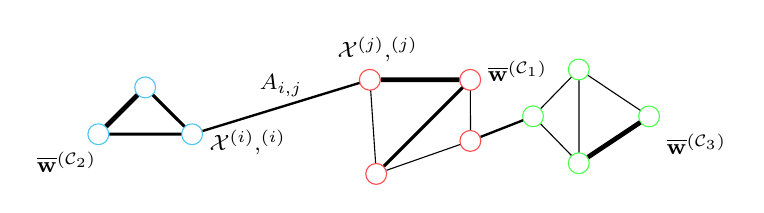
\begin{tikzpicture}[scale=8/5]
\tikzstyle{every node}=[font=\small]
%\draw[darkgray, fill=cyan!5, densely dashed] (1.2,1.2) circle (1.4);
%\draw[shift ={(3.5,0)}] [darkgray, densely dashed]  (1.2,1.2) circle (1.4);
\node[nred] (C1_2) at (0.88+3.7,2.29) {};
\node[left=1 cm of C1_2,nred] (C1_1)  {};
\node[below left =1cm and 1cm of C1_2,nred] (C1_3)  {};
\node[below =0.5cm of C1_2,nred] (C1_4)  {};
\node[ngreen] (C3_3) at (6,2) {};
\node[above left =0.4cm and 0.7cm of C3_3,ngreen] (C3_2)  {};
\node[below left =0.4 and 0.7cm of C3_3,ngreen] (C3_4) {};
\node[left =1.2cm of C3_3,ngreen] (C3_1) {};
\node[ncyan] (C2_2) at (2.0,2.23) {};
\node[below left =0.4cm and 0.4cm of C2_2,ncyan] (C2_1)  {};
\node[below right =0.4cm and 0.4cm of C2_2,ncyan] (C2_3)  {};
\node[below right = 0.01cm and 0.00cm of C2_3, font=\fontsize{8}{0}\selectfont,anchor=west] {$\mathcal{X}^{(i)}, \vw^{(i)}$}; 
\node[above right = 0.01cm and 0.00cm of C1_1, font=\fontsize{8}{0}\selectfont,anchor=south] {$\mathcal{X}^{(j)}, \vw^{(j)}$}; 
\node[above right = 0.01cm and 0.00cm of C1_2, font=\fontsize{8}{0}\selectfont,anchor=west] {$\overline{\mathbf{w}}^{(\mathcal{C}_1)}$}; 
\node[below right = 0 and 0.00cm of C2_1,font=\fontsize{8}{0}\selectfont,anchor=north east] {$\overline{\mathbf{w}}^{(\mathcal{C}_2)}$}; 
\node[below right = 0 and 0.0cm of C3_3,font=\fontsize{8}{0}\selectfont,anchor=north west]  {$\overline{\mathbf{w}}^{(\mathcal{C}_3)}$}; 

\draw [line width=0.3mm,-] (C2_3)--(C1_1) node[draw=none,fill=none,font=\fontsize{8}{0}\selectfont,midway,above] {$A_{i,j}$};
\draw [line width=0.6mm,-] (C1_2)--(C1_1);
\draw [line width=0.4mm,-] (C1_2)--(C1_3);
\draw [-] (C1_1)--(C1_3);
\draw [-] (C1_3)--(C1_4);
\draw [-] (C1_2)--(C1_4);
\draw [line width=0.3mm,-] (C1_4)--(C3_1);
\draw [line width=0.6mm,-] (C2_1)--(C2_2);
\draw [line width=0.4mm,-] (C2_2)--(C2_3);
\draw [line width=0.4mm,-] (C2_1)--(C2_3);
\draw [-] (C3_1)--(C3_2);
\draw [-] (C3_2)--(C3_3);
\draw [line width=0.6mm,-] (C3_3)--(C3_4);
\draw [-] (C3_2)--(C3_4);
\draw [-] (C3_1)--(C3_4);
\end{tikzpicture}
\caption{\label{fig_local_dataset} We represent networked data and corresponding models using an undirected empirical graph $\graph=\big(\nodes,\edges\big)$. 
	Each node $\nodeidx \in \nodes$ of the graph carries a local dataset $\localdataset{\nodeidx}$ and model weights $\localparams{\nodeidx}$ which 
	are scored using a local loss function $\locallossfunc{\nodeidx}{\localparams{\nodeidx}}$ (that encapsulates the local dataset $\localdataset{\nodeidx}$). 
	Two nodes are connected by a weighted edge $\{\nodeidx,\nodeidx'\}$ if they carry datasets with similar statistical properties. 
	The amount of similarity is encoded in an edge weight $\edgeweight_{\nodeidx,\nodeidx'}>0$ (indicated by thickness of the links). 
	We rely on a clustering assumption, requiring optimal parameter vectors for nodes in the same cluster 
	$\cluster{\clusteridx} \subseteq \nodes$ to be nearly identical. 
	The empirical graph is partitioned into three disjoint clusters $\cluster{1},\cluster{2},\cluster{3}$. 
	Note that our FL method does not require the (typically unknown) partition but rather learns the 
	partition based on the local datasets and network structure of $\graph$. 
}
\end{center}
\vspace{-3mm}
\end{figure} 

An undirected edge $\{\nodeidx,\nodeidx'\}\!\in\!\edges$ indicates that the corresponding local 
datasets $\localdataset{\nodeidx}$ and $\localdataset{\nodeidx'}$ have similar statistical properties. 
The strength of the similarity is quantified by the edge weight $\edgeweight_{\nodeidx,\nodeidx'}\!>\!0$. 
We will also use the notation $\edgeweight_{\edgeidx} \defeq  \edgeweight_{\nodeidx,\nodeidx'}$ for 
an edge $\edgeidx = \edge{\nodeidx}{\nodeidx'}$. 
It will be convenient to indicate absence of an edge between two nodes $\nodeidx,\nodeidx' \in \nodes$ 
by a zero weight, i.e., $\edgeweight_{\nodeidx,\nodeidx'} = 0$ if and only if $\{\nodeidx,\nodeidx'\} \notin \edges$. 

The undirected edge $\edge{\nodeidx}{\nodeidx'} \in \edges$ encodes a symmetric notion of similarity 
between local datasets. If the local dataset at node $\nodeidx$ is (statistically) similar to the local 
dataset at node $\nodeidx'$ then also vice-versa. The symmetric nature of the similarities between 
local datasets is also reflected in the edge weights, 
\vspace{-2mm}
$$\edgeweight_{\nodeidx,\nodeidx'} = \edgeweight_{\nodeidx', \nodeidx} \mbox{ for any two nodes } \nodeidx, \nodeidx' \in \nodes. \vspace{-2mm}$$
%Despite the symmetric notion of similarity encoded in the empirical graph $\graph=\pair{\nodes}{\edges}$, 
It will be convenient for the formulation and analysis of our NFL algorithm (see Algorithm \ref{alg1}) 
to orient the edges in $\edges$. 
In particular, we define the head and tail of an undirected edge $\edgeidx=\{\nodeidx,\nodeidx'\} \in \edges$ 
as $\edgeidx_{+} \defeq \min\{\nodeidx,\nodeidx'\}$ and $\edgeidx_{-} \defeq \max\{\nodeidx,\nodeidx'\}$, respectively. 
The entire set of directed edges for an empirical graph is obtained as  
\begin{equation} 
	\label{equ_def_directed_edges_empgraph}
\overrightarrow{\edges} \defeq \big\{\directededge{\nodeidx}{\nodeidx'}: \nodeidx,\nodeidx' \in \nodes, \nodeidx < \nodeidx' \mbox{ and } \edge{\nodeidx}{\nodeidx'} \in \edges \big\}. 
\end{equation} 
We abuse notation and use $\edges$ not only to denote the set of undirected edges but 
also to denote the set \eqref{equ_def_directed_edges_empgraph} of directed edges in the empirical graph $\graph$. 
 
There are two vector spaces that are naturally associated with an empirical graph $\graph$. 
The ``node space'' $\nodespace$ consists of maps 
$\netparams: \nodes \rightarrow \mathbb{R}^{\dimlocalmodel}: \nodeidx \mapsto \localparams{\nodeidx}$
that assign each node $\nodeidx \in \nodes$ a vector $\localparams{\nodeidx} \in \mathbb{R}^{\dimlocalmodel}$. 
The ``edge space'' $\edgespace$ of all maps 
$\vu: \edges \rightarrow \mathbb{R}^{\dimlocalmodel}: \edgeidx \mapsto \localflowvec{\edgeidx} $
that assign each edge $\edgeidx \in \edges$ a vector $\localflowvec{\edgeidx} \in \mathbb{R}^{\dimlocalmodel}$. 
These two spaces are linked via the block-incidence matrix $\incidencemtx$ with entries 
$\incidencemtxentry{\edgeidx}{\nodeidx} = 1$ for $\nodeidx = \edgeidx_{+}$, $\incidencemtxentry{\edgeidx}{\nodeidx} = -1$ for $\nodeidx = \edgeidx_{-}$, and $\incidencemtxentry{\edgeidx}{\nodeidx} = 0$ otherwise.
% $$ \incidencemtxentry{\edgeidx}{\nodeidx} = \begin{cases} 1 & \mbox{ for } \nodeidx = \edgeidx_{+} \\ -1 & \mbox{ for } \nodeidx = \edgeidx_{-} \\ 0 & \mbox{ otherwise.} \end{cases}$$ 
The  block-incidence matrix $\incidencemtx$ represents a linear map 
\vspace{-2mm}
\begin{equation}
\label{equ_def_block_incidence_matrix}
 \mD: \nodespace \rightarrow \edgespace: \netparams \mapsto \flowvec \mbox{ with } \localflowvec{\edgeidx} = \localparams{\edgeidx_{+}} - \localparams{\edgeidx_{-}} %  ^{(e_{+})} -  \vw^{(e_{-})} $. 
 %   D_{e, i} =  {\bf I} \mbox{ for } i\!=\!e_{+},  D_{e, i} =  -{\bf I} \mbox{ for } i\!=\!e_{-} \mbox{ and }  D_{e, i} =\mathbf{0} \mbox{ otherwise.}
 \vspace{-2mm}
 \end{equation} 
with the adjoint (transpose) $\incidencemtx^{T}$ representing another linear map, 
 \begin{equation}
 \label{equ_def_block_incidence_transp_matrix}
 	\incidencemtx^{T}: \edgespace \rightarrow \nodespace: \flowvec \mapsto \netparams \mbox{ with } \localparams{\nodeidx} = \sum_{\edgeidx \in \edges} 
 	\sum_{\nodeidx = \edgeidx_{+}} \localflowvec{\edgeidx} - \sum_{\nodeidx = \edgeidx_{-}}  \localflowvec{\edgeidx}.
  \vspace{-4mm}
 \end{equation} 


\subsection{Networked Models}
\label{sec_net_models}

A networked model consists of a separate local model for each local dataset $\localdataset{\nodeidx}$. 
Our approach to NFL allows for a large variety of design choices for the local models. We only 
require all local models to be parametrized by a common finite-dimensional Euclidean space $\mathbb{R}^{\dimlocalmodel}$. 
This setting covers some widely-used ML models such as (regularized) generalized linear 
models or linear time series models \cite{LocalizedLinReg2019,Brockwell91}. 
However, our setting does not cover non-parametric local models such as decision trees. 

Networked models are parametrized by a map $\netparams \in \nodespace$ that assigns each node $\nodeidx \in \nodes$ 
in the empirical graph $\graph$ a local model parameter vector $\localparams{\nodeidx} \in \mathbb{R}^{\dimlocalmodel}$, \footnote{With 
	a slight abuse of notation we will refer by $\localparams{\nodeidx}$ also to the entire collection of local model parameters.}
$\weights: \nodes \rightarrow \mathbb{R}^{\dimlocalmodel}: \nodeidx \mapsto \weights^{(\nodeidx)}.$
%The main theme of this paper is to study conditions on the network 
%For a given node $i \in \nodes$, the predictor \eqref{equ_def_node_predictor} reads in the feature 
%vector $\vx$ of an arbitrary datapoint (which might be outside the local dataset $\localdata{i}$) 
%and outputs a prediction $h(\vx;\vw^{(i)})$. The node-wise predictor \eqref{equ_def_node_predictor} 
%is parametrized by the node-wise weight vector $\vw^{(i)}$. Thus, learning an accurate 
%predictor \eqref{equ_def_node_predictor} is equivalent to learning its weight vector $\vw^{(i)}$. 
%
%For numeric labels $y \in \mathbb{R}$, we use the output $h(\vx;\vw^{(i)})$ directly
%as the predicted label $\hat{y}=h(\vx;\vw^{(i)})$. For applications involving binary labels
%$y \in \{-1,1\}$ we classify $\hat{y} = 1$ for $h(\vx;\vw^{(i)}) \geq 0$ and $\hat{y} = -1$
%otherwise. For applications where local datasets represent humans, we might
%refer to the local predictors $h(\vx;\vw^{(i)})$, for $i \in \nodes$, as personalized predictors.
We measure the usefulness of a particular choice for the local model parameters $\localparams{\nodeidx}$ 
by some local loss function $\locallossfunc{\nodeidx} {\localparams{\nodeidx}}$. Unless stated otherwise, 
we consider local loss functions that are convex and differentiable. The NFL method proposed in 
Section \ref{sec_federatedml} allows for different choices for the local loss functions. These different choices 
might be obtained, in turn, from different combinations of ML models and performance metrics \cite[Ch. 3]{MLBasics}. 

From a computational perspective, our main requirement on the choice for the local loss function 
$\locallossfunc{\nodeidx} {\localparams{\nodeidx}}$ is that it allows for efficient solution of the regularized problem, 
\begin{equation}
\label{equ_def_reguarlizated-local_loss}
	\min_{\weights' \in \mathbb{R}^{\dimlocalmodel}}  \locallossfunc{\nodeidx} {\weights'}+ \regparam \| \weights' - \weights'' \|^{2}_{2}. 
 \vspace{-2mm}
\end{equation} 
The computational complexity of our approach depends on the ability to efficiently solve 
\eqref{equ_def_reguarlizated-local_loss} for any given $\regparam \in \mathbb{R}_{+}$ 
and $\weights'' \in \mathbb{R}^{\dimlocalmodel}$. Note that solving \eqref{equ_def_reguarlizated-local_loss} 
is equivalent to evaluating the proximity operator $\proximityop{\locallossfunc{\nodeidx}{\cdot}}{\weights''}{2 \regparam}$. %of $(2/\regparam)\locallossfunc{\nodeidx}{\cdot}$ \cite{ProximalMethods}. 

The NFL method in Section \ref{sec_federatedml} applies to parametric models that can be trained 
by minimizing a loss function $\locallossfunc{\nodeidx}{\cdot}$ whose proximity operator can be evaluated efficiently. 
Convex functions for which the proximity operator can be computed efficiently are sometimes referred 
to as ``proximable'' or ``simple'' \cite{Condat2013}. Note that the shape of the loss function typically 
depends on both, the choice for the local model and the metric used to measure prediction errors \cite[Ch.\ 4]{MLBasics}. 

Our focus is on applications where the local loss functions $\locallossfunc{\nodeidx}{\localparams{\nodeidx}}$ 
do not carry sufficient statistical power to guide learning of model parameters $\localparams{\nodeidx}$. As a 
case in point, consider a local dataset $\localdataset{\nodeidx}$ of the form \eqref{equ_def_local_dataset_plain}, with 
feature vectors $\featurevec^{(\sampleidx)} \in \mathbb{R}^{\dimlocalmodel}$ with $\localsamplesize{\nodeidx} \ll \dimlocalmodel$. 
We would like to learn the parameter vector $\localparams{\nodeidx}$ of a linear hypothesis $h(\featurevec) =\big( \localparams{\nodeidx} \big)^{T}   \featurevec$. Linear regression methods learn the parameter vector by minimizing the average  
squared error loss $\locallossfunc{\nodeidx}{\localparams{\nodeidx}}=(1/\samplesize_{\nodeidx}) \sum_{\sampleidx=1}^{\localsamplesize{\nodeidx}} \big( \truelabel^{(\sampleidx)} - \big( \localparams{\nodeidx} \big)^{T} \featurevec^{(\sampleidx)} \big)^{2}$. 
However, for $\localsamplesize{\nodeidx} \ll \dimlocalmodel$ (the ``high-dimensional'' regime) the minimum of 
$\locallossfunc{\nodeidx}{\cdot}$ is not unique and might also provide a poor hypothesis incurring large 
prediction errors on data points outside $\localdataset{\nodeidx}$
\cite[Ch. 6]{MLBasics}. Training linear models in the high-dimensional regime requires regularization such as in 
ridge regression or Lasso \cite{hastie01statisticallearning}. 

%One form of regHere, we need to pool local datasets that have similar statistical properties as $\localdataset{\nodeidx}$ 
%to obtain a sufficiently large training set for learning the parameter vector of a linear hypothesis. 
The main theme of this paper is to use the empirical graph $\graph$ to regularize the learning 
of local model parameters by requiring them to not vary too much over edges with large weights. 
Section \ref{sec_nLasso} introduces the concept of GTV as a quantitative measure for the variation 
of local parameter vectors. Regularization by requiring a small GTV is an instance of the 
smoothness assumption used in semi-supervised learning \cite{SemiSupervisedBook}. 

Our analysis of GTV minimization in Section \ref{sec_when_does_it_work} relates its underlying 
smoothness assumption to a clustering assumption. Section \ref{sec_clustering_assumption} formalizes 
this clustering assumption which requires local model parameters to be constant over subsets (clusters) 
of nodes in the empirical graph. Theorem \ref{thm_main_result} then offers precise conditions on the 
empirical graph and local loss functions such that GTV minimization successfully recovers the clusters 
of nodes.

\subsection{Clustering Assumption}
\label{sec_clustering_assumption}
%The criterion \eqref{eq:4} alone is insufficient to guide the learning of the weights $\vw^{(i)}$
%since it completely ignores the weights $\vw^{(i)}$ at nodes $i \in \nodes \backslash \trainingset$ outside 
%the training set. We therefore need to impose some additional structure on the collection of 
%weight vectors $\vw^{(i)}$, for $i \in \nodes$. To this end, we exploit the network structure of 
%the empirical graph $\graph$. 
Consider networked data with empirical graph $\graph = \pair{\nodes}{\edges}$. 
Each node $\nodeidx$ in the graph carries a local dataset $\localdataset{\nodeidx}$ and a local model with parameters 
$\localparams{\nodeidx}$. Our goal is to learn the local model parameters $\localparams{\nodeidx}$ for each node $\nodeidx \in \nodes$. 
The key assumption of clustered FL is that the local datasets form clusters with local datasets in the same 
cluster having similar statistical properties \cite{NIPS2008_fccb3cdc}. Given a 
cluster $\clustergeneric$ of nodes, it seems natural to pool their local datasets or, equivalently, add their 
local functions to learn a cluster-specific parameter vector 
\begin{equation} 
	\label{equ_def_opt_cluster}
	\overline{\weights}^{(\clustergeneric)} =  \argmin_{\vv \in \mathbb{R}^{\dimlocalmodel}} \clusterobj{\clustergeneric}{\vv} \mbox{ with } \clusterobj{\clustergeneric}{\vv} \defeq \sum_{\nodeidx \in \clustergeneric}\locallossfunc{\nodeidx}{\vv}.
 \vspace{-2mm}
\end{equation}
Note that \eqref{equ_def_opt_cluster} cannot be implemented in practice since we typically do not know 
the cluster $\clustergeneric$. The main analytical contribution of this paper is an upper bound for the deviation 
between solutions of GTV minimization and the cluster-wise (but impractical) learning problem \eqref{equ_def_opt_cluster}. 
This bound characterizes the statistical properties of FL algorithms that are obtained by applying 
optimization techniques for solving GTV minimization (see Section \ref{sec_federatedml}). 

The solution $\overline{\weights}^{(\clustergeneric)}$ of \eqref{equ_def_opt_cluster} minimizes the 
aggregation (sum) of all local loss functions that belong to the same cluster $\clustergeneric \subseteq \nodes$. 
Thus, $\overline{\weights}^{(\clustergeneric)}$ is the optimal model parameter for a training set obtained by 
pooling all local datasets that belong to the cluster $\clustergeneric$. As indicated by our notation, we 
tacitly assume that the solution to \eqref{equ_def_opt_cluster} is unique. The uniqueness of the 
solution in \eqref{equ_def_opt_cluster} will be ensured by Assumption \ref{asspt_FIM_lower_bound} below. 

We now make our assumption of datasets in the same cluster ``having similar statistical properties'' precise. 
In particular, we require the local loss functions at nodes $\nodeidx \in \clustergeneric$ in the same cluster $\clustergeneric$ 
to have nearby minimizers. Thus, we require a small deviation $\normgeneric{\vv^{(\nodeidx)} - \overline{\weights}^{(\clustergeneric)}}{}$ 
between the minimizer $\vv^{(\nodeidx)}$ of $\locallossfunc{\nodeidx}{\cdot}$ and the corresponding 
cluster-wise optimal parameter vector \eqref{equ_def_opt_cluster}. This requirement is, for differentiable and convex loss 
functions, equivalent to requiring a small gradient of the local loss functions at the cluster-wise 
minimizer \eqref{equ_def_opt_cluster}. It will be convenient for our analysis to formulate this 
requirement by upper bounding the dual norm $\normgeneric{\nabla \locallossfunc{\nodeidx}{\overline{\weights}^{(\clustergeneric)}} }{*}$ 
of the local loss gradient. 
 %For a specific 
%cluster $\cluster$, the collection of loss functions $\big\{ \locallossfunc{\nodeidx}{\cdot}\big\}_{\nodeidx \in \cluster}$ 
%can be simultaneously minimized by the solution of the cluster-wide minimization problem 
%We now make our clustering assumption precise. 
\begin{assumption}[Clustering]
\label{asspt_weights_clustered}
Consider some networked data represented by an empirical graph $\graph$ whose nodes 
carry local loss functions $\locallossfunc{\nodeidx}{\vv}$, for $\nodeidx \in \nodes$. 
There is a partition of the nodes $\nodes$ into disjoint clusters 
\begin{equation}
\label{equ_def_parition_asspt}
\begin{aligned}
 &{\partition\!=\!\{\cluster{1},\ldots,\cluster{\nrcluster} \} \mbox{ with } \cluster{\clusteridx} \cap \cluster{\clusteridx'} = \emptyset ,} \\
 &{ \quad \mbox{ for } \clusteridx\!\neq\!\clusteridx' \mbox{ and } \nodes = \cluster{1} \cup \ldots \cup \cluster{\nrcluster}.} 
\end{aligned}
 \vspace{-2mm}
\end{equation} 
Moreover, for each cluster $\cluster{\clusteridx}\in \partition$, 
\begin{equation}
\label{equ_upper_bound_norm_gradient}
\normgeneric{\nabla \locallossfunc{\nodeidx}{\overline{\weights}^{(\clusteridx)}} }{*}  \leq \clusteropterr{\nodeidx} \mbox{ for all } \nodeidx \in \cluster{\clusteridx}. 
 \vspace{-2mm}
\end{equation}
Here, $\overline{\weights}^{(\clusteridx)}\!\in\!\mathbb{R}^{\dimlocalmodel}$ denotes the solution of the cluster-wise minimization
\eqref{equ_def_opt_cluster} for cluster $\cluster{\clusteridx}$. 
\end{assumption} 
The clustering assumption requires the dual norm $\normgeneric{\nabla \locallossfunc{\nodeidx}{\ \overline{\weights}^{(\clusteridx)}}}{*}$ 
to be bounded by a constant $\clusteropterr{\nodeidx}$ for each nodes $\nodeidx \in \nodes $ in the empirical graph. 
We can interpret this norm as a measure for the discrepancy between the cluster-wise minimizer $\overline{\weights}^{(\clusteridx)}$ 
(see \eqref{equ_def_opt_cluster}) and the minimizers of the local loss functions $\locallossfunc{\nodeidx}{\overline{\weights}^{(\clusteridx)}}$ 
for each node $\nodeidx \in \cluster{\clusteridx}$. 

%This amounts to a partition $\nodes = \cluster_{1} \cup,\ldots,$,  of the nodes in $\graph$ into mutually disjoint clusters $\cluster_{1},\ldots,$, 
%We assume that the nodes cluters $\cluster{},\ldots,\cluster{\nrcluster}$ 
%such that local datasets in the same empirical graph can be decomposed into few tight-knit clusters. 
Section \ref{sec_federatedml} uses the cluster-wise minimization \eqref{equ_def_opt_cluster} as a 
theoretical device to analyze the solutions of GTV minimization \eqref{equ_gtvmin}. It is important to 
note that \eqref{equ_def_opt_cluster} does not inform a practical FL method as it requires knowledge 
of the clusters in the partition \eqref{equ_def_parition_asspt}. It might be unrealistic to assume perfect 
knowledge of the partition \eqref{equ_def_parition_asspt} postulated by Assumption \ref{asspt_weights_clustered}. 
Rather, we show that GTV minimization is able to recover this partition using solely the edges of the empirical 
graph $\graph$. 

Section \ref{sec_nLasso} formulates NFL as GTV minimization which is an instance of RERM. GTV minimization is 
enforces ``clusteredness'' of local model parameters by requiring a small variation across edges in the 
empirical graph. Under Assumption \ref{asspt_weights_clustered}, this regularization strategy will be useful if many (large weight) 
edges connect nodes in the same cluster but only few (small weight) edges connect nodes in different clusters. 
Section \ref{sec_when_does_it_work} presents a precise condition on the network structure such that GTV 
minimization succeeds in capturing the true underlying cluster structure of the local loss functions. 

% NFL methods that use the network structure of the empirical graph 
%to jointly cluster the nodes and optimize the parameter vectors $\localparams{\nodeidx}$ of the local models.   
%In particular, these methods use GTV to measure the clusteredness of a given collection of local model parameters 
%and, in turn, regularize the learning of them. Section \ref{} will discuss the resulting GTV minimization problem 

%do not require the knowledge of clusters but use the network 
%We then require the weight vectors $\vw^{(i)}$ to be approximately 
%constant for all nodes $i \in \nodes$ belonging to the same cluster. 

The analysis of the NFL method proposed in Section \ref{sec_when_does_it_work} requires the 
local loss functions to be convex and smooth. Moreover, we require their (partial) sums in the cluster-wise 
objective $\clusterobj{\clusteridx}{\cdot}$ \eqref{equ_def_opt_cluster} to be strongly 
convex \cite[Exercise 1.9]{BertCvxAnalOpt}. 
\begin{assumption}[Convexity and Smoothness]
	\label{asspt_FIM_lower_bound}
%	For each node $\nodeidx \in \nodes$, the local loss $\locallossfunc{\nodeidx}{\vv}$ is a convex 
% smooth function.
For each node $\nodeidx \in \nodes$, the local loss function $\locallossfunc{\nodeidx}{\localparams{\nodeidx}}$ is convex 
and differentiable with gradient satisfying 
\begin{equation}
	\label{equ_def_cond_locallipsch}
\normgeneric{ \nabla \locallossfunc{\nodeidx}{\vv'} - \nabla \locallossfunc{\nodeidx}{\vv}}{*} \leq \locallipsch{\nodeidx} \normgeneric{\vv'- \vv}{}. 
 \vspace{-2mm}
\end{equation} 
%Consider the partition \eqref{equ_def_parition_asspt} of the empirical graph and the associated cluster-wide 
%loss functions $\clusterobj{\clusteridx}{\cdot}$.
For each cluster $\cluster{\clusteridx} \in \partition$ in the partition \eqref{equ_def_parition_asspt}, 
the cluster-wise objective $\clusterobj{\clusteridx}{\cdot}$ \eqref{equ_def_opt_cluster} is strongly convex, 
%twice-differentiable with partial derivatives 
%$\frac{\partial^{2}{\clusteridx}{\vv} }{\partial v_{r} \partial v_{s}}$ that constitute 
%the Hessian $\nabla^{2} \clusterobj{\clusteridx}{\vv}$. The eigenvalues of the Hessian are 
%uniformly lower bounded as %given  is twice-differentiable and satisfies 
\begin{equation} 
\label{equ_strong_convexit}
\begin{aligned}
    \clusterobj{\clusteridx}{\vv'} \geq \clusterobj{\clusteridx}{\vv}  +
 &{\big( \vv' \!-\! \vv \big)^{T} \partial \clusterobj{\clusteridx}{\vv} + (\strongconvparam{\clusteridx}/2) \norm{\vv' \!-\! \vv}^{2},} \\
 &{\mbox{ for any } \vv', \vv \in \mathbb{R}^{\dimlocalmodel}.} 
\end{aligned}
 \vspace{-2mm}
\end{equation} 
Here, $\strongconvparam{\clusteridx}> 0$ is a positive constant that might be different for different clusters $\cluster{\clusteridx}$. 
The norm $\normgeneric{\cdot}{}$ in \eqref{equ_def_cond_locallipsch}, \eqref{equ_strong_convexit} is the dual of 
the norm $\normgeneric{\cdot}{*}$ used in \eqref{equ_def_cond_locallipsch} and \eqref{equ_upper_bound_norm_gradient}. 
\end{assumption}  
%The factor $2$ in \eqref{equ_bound_eigs_FIM} is only for notational convenience. 
Assumption \ref{asspt_FIM_lower_bound} is rather standard in FL literature \cite{Ghosh2020,Nassif2020}. 
In particular, Assumption \ref{asspt_FIM_lower_bound} is satisfied by many important ML models \cite{LocalizedLinReg2019}. 
Assumption \ref{asspt_FIM_lower_bound} does not hold for many deep learning models that result in 
non-convex loss functions \cite{pmlr-v54-mcmahan17a}. Nevertheless, we expect our theoretical analysis 
to provide useful insight also for settings where Assumption \ref{asspt_FIM_lower_bound} is violated.  

%??? can we show this in experiments ???? Yu, Yasmin ??? 

We emphasize that Assumption \ref{asspt_FIM_lower_bound} does not require strong convexity for each local loss 
function $\locallossfunc{\nodeidx}{\cdot}$ individually. Rather, it only requires their cluster-wise sums \eqref{equ_def_opt_cluster} 
to be strongly convex. We also allow for trivial local loss functions that are constant and might represent 
inaccessibility of local datasets due to  privacy-constraints or lack of computational resources. 

The NFL method in Section \ref{sec_federatedml} can tolerate the presence of non-informative local loss functions by exploiting the 
similarities between local datasets as reflected by the edges in the empirical graph $\graph$. Supplementary material \ref{ref_some_special_cases} 
presents examples for local loss functions, obtained from some widely-used ML models, that conform 
to Assumption \ref{asspt_FIM_lower_bound}. %In particular, for linear regression 
%the condition \eqref{equ_bound_eigs_FIM} is satisfied with high probability if the features of data points are 
%not too strongly correlated (see Appendix \ref{ref_some_special_cases}).

%To evaluate the overall quality of networked model parameters $\localparams{\nodeidx}$, 
%we compute the training error
%\begin{equation} \label{eq:4}
%f(\vw) \defeq \sum_{i \in \trainingset} \mathcal{L}^{(i)} \big(\vw^{(i)} \big). 
%\end{equation}
%Here we used the shorthand $\mathcal{L}^{(i)} \big(\vw^{(i)} \big) \defeq \mathcal{L} \big(\mathcal{X}^{(i)};\vw^{(i)} \big)$. 
%Unless noted otherwise, we assume that $\mathcal{L}^{(i)} \big(\cdot \big)$, for $i \in \nodes$ are convex functions. 
%Additional restrictions are placed on $\mathcal{L}^{(i)} \big(\cdot \big)$ in Section \ref{equ_analysis_error} to facilitate 
%the analysis of statistical properties of our proposed algorithm. 
%This algorithm aims at learning networked weights $\weights$ such that the training error \eqref{eq:4} is small. 

\section{Generalized Total Variation Minimization}
\label{sec_nLasso}

The clustering Assumption \ref{asspt_weights_clustered} suggests to learn the model parameters $\localparams{\nodeidx}$ via 
the cluster-wise optimization \eqref{equ_def_opt_cluster}. For each cluster $\cluster{\clusteridx}$ in the partition \eqref{equ_def_parition_asspt}, 
we use the solution of \eqref{equ_def_opt_cluster} as the local model parameters at all nodes $\nodeidx \in \cluster{\clusteridx}$. 
However, this approach is not practical since the partition \eqref{equ_def_parition_asspt} is typically unknown and therefore 
we cannot directly implement \eqref{equ_def_opt_cluster}. Instead, we use the empirical graph $\graph$ to penalize variations 
of local model parameter $\localparams{\nodeidx}$ over well-connected nodes (see Section \ref{sec_primal_problem}). 

We hope that penalizing their variation (over the edges in the empirical graph) favours local model parameters 
that are approximately constant over nodes in the same cluster \eqref{equ_def_parition_asspt}. For this approach 
to be successful, the nodes in the same cluster must be densely connected by many edges (or large weight) in 
the empirical graph, which should have only few edges (with low weight) between nodes in different clusters. 
We will make this informal assumption precise in Section \ref{sec_when_does_it_work}. For now, we use the 
informal clustering assumption to motivate GTV as a useful regularizer for learning the local model parameters. 

If the cluster structure of $\graph$ is reflected by a high density of edges within clusters and  
few boundary edges between them, it seems reasonable to require a small variation of local 
parameter vectors $\localparams{\nodeidx}$ across edges. We measure the variation of local parameter 
vectors $\netparams \in \nodespace$ across the edges in $\graph$ via the variation $\flowvec: \edgeidx \in \edges \mapsto \localflowvec{\edgeidx} \defeq \localparams{\edgeidx_{+}} -  \localparams{\edgeidx_{-}}$. 
Using the block-incidence matrix \eqref{equ_def_block_incidence_matrix} we can express the variation of $\netparams$
more compactly as $\flowvec = \incidencemtx \netparams$. 

A quantitative measure for the variation of local model parameters $\netparams$ is the GTV
\begin{equation} \label{eq:5}
\begin{aligned}
    &{\normgeneric{\weights}{\rm GTV}   \defeq \sum_{\edge{\nodeidx}{\nodeidx'} \in \edges} \edgeweight_{\nodeidx,\nodeidx'} \phi\big(\localparams{\nodeidx'} -\localparams{\nodeidx}  \big) }
    % &{\mbox{ with some convex penalty function } \gtvpenalty(\cdot): \mathbb{R}^{\dimlocalmodel} \rightarrow \mathbb{R}.}
\end{aligned}
\vspace{-2mm}
\end{equation}
 with some convex penalty function $\gtvpenalty(\cdot): \mathbb{R}^{\dimlocalmodel} \rightarrow \mathbb{R}$.
We also define the GTV for a subset of edges $\mathcal{S} \subseteq \edges$ as 
\begin{equation} \label{eq:def_GTV_subset}
	\| \weights \|_{\mathcal{S}}  \defeq \sum_{\edge{\nodeidx}{\nodeidx'} \in \mathcal{S}} \edgeweight_{\nodeidx,\nodeidx'} \gtvpenalty\big(\localparams{\nodeidx'} -\localparams{\nodeidx}  \big).
 \vspace{-2mm}
\end{equation} 
The GTV \eqref{eq:5} provides a whole ensemble of variation measures. This ensemble is parametrized by a 
penalty function $\gtvpenalty(\vv) \in \mathbb{R}$ which we tacitly assume to be convex. The penalty 
function $\gtvpenalty(\cdot)$ is an important design choice that determines the computational and 
statistical properties of the resulting GTV minimization problem (see Section \ref{sec_federatedml} 
and Section \ref{sec_when_does_it_work}). Two popular choices are $\gtvpenalty(\vv) \defeq \| \vv\|_{2}$, 
which is used by nLasso \cite{NetworkLasso}, and $\gtvpenalty(\vv) \defeq (1/2)\| \vv\|^{2}_{2}$ 
which is used by the method {\rm MOCHA} \cite{Smith2017}. Another recent FL method for networked data uses 
the choice $\gtvpenalty(\vv) \defeq \| \vv \|_{1}$ \cite{Sarchesh2021}. 

Different choices for the penalty function offer different trade-offs between computational complexity and 
statistical properties of the resulting FL algorithms. As a case in point, the penalty $\gtvpenalty(\flowvec)= \|\flowvec\|_{2}$ (used in nLasso) 
is computationally more challenging than the penalty $\gtvpenalty(\vu)= (1/2) \|\flowvec\|_{2}^{2}$ (used in {\rm MOCHA} \cite{Smith2017}). 
On the other hand, nLasso is more accurate in learning models for data with specific 
network structures (such as chains) that are challenging for GTV minimization method using the 
smooth penalty $\gtvpenalty(\vv) \defeq (1/2)\| \vv\|^{2}_{2}$ \cite{WhenIsNLASSO}.  

Section \ref{sec_federatedml} designs FL methods whose main computational steps include the computation of 
the proximity operator $\proximityop{\phi^{*}}{\cdot}{\rho}$ for the convex conjugate $\gtvpenalty^{*}$ of the 
GTV penalty function $\gtvpenalty(\cdot)$. Thus, for these methods to be computationally tractable we must 
choose $\gtvpenalty(\cdot)$ such that the proximity operator $\proximityop{\phi^{*}}{\cdot}{\rho}$ can be computed (evaluated) efficiently.\footnote{The difficulty 
	of computing the proximity operator $\proximityop{\phi^{*}}{\vu}{\rho}$ is essentially the same as that 
	of computing the proximity operator $\proximityop{\phi}{\vu}{\rho}$. Indeed, these two proximity operators 
	are related via the identity $\vu = \proximityop{\phi}{\vu}{1}+ \proximityop{\phi^{*}}{\vu}{1}$  \cite{ProximalMethods}.}
Supplementary material \ref{ref_penalty_some_special_cases} discusses some choices for the GTV penalty function $\gtvpenalty(\cdot)$ 
for which this is the case. 

%  Our analysis in Section \ref{} For our analysis of NFL methods in Section \ref{}
\subsection{The Primal Problem}
\label{sec_primal_problem}
%To learn the weights $\mathbf{w}^{(i)}$ of the local models, one for each local dataset $\mathcal{X}^{(i)}$. 
%we assume that local datasets forming a tight-knit subset (or cluster) $\cluster \subseteq \nodes$ have similar 
%statistical properties. 
%The clustering Assumption \ref{asspt_weights_clustered} suggests to learn the local model parameters by 
%solving the cluster-wide learning problems \eqref{equ_def_opt_cluster}. However, \eqref{equ_def_opt_cluster} 
%is not feasible, since we do not know the partition \eqref{equ_def_parition_asspt} of local datasets into clusters. 
%Instead, we penalize the sum of local loss functions by the GTV of the local model parameters $\localparams{\nodeidx}$. 
%
%
%Our goal is to learn similar local model parameters $\localparams{\nodeidx}\!\approx\!\localparams{\nodeidx'}$ for nodes 
%$\nodeidx,\nodeidx' \in \nodes$ in the same cluster $\cluster{\clusteridx}$.  we require a small GTV  $\| \weights \|_{\rm GTV}$ \eqref{eq:5}. 
%The extreme case of vanishing GTV $\| \weights \|_{\rm GTV}=0$ is achieved by using identical 
%local parameter vectors $\localparams{\nodeidx} =\localparams{\nodeidx'}$ for all nodes $\nodeidx,\nodeidx' \in \nodes$. 
%However, we also need to take into account the local loss functions $\locallossfunc{\nodeidx}{\localparams{\nodeidx}}$ 
%whose minimizers differ for nodes in different clusters (see Assumption \ref{}). 

GTV minimization learns the local model parameters $\localparams{\nodeidx}$ by balancing (the sum of) 
local loss functions and GTV \eqref{eq:5}, 
\begin{equation} 
\label{equ_gtvmin}
\widehat{\netparams} \in \underset{\netparams \in \nodespace}{\mathrm{arg \ min}}\sum_{\nodeidx \in \nodes} \locallossfunc{\nodeidx}{\localparams{\nodeidx}} + \regparam \|\netparams\|_{\rm GTV}.
\vspace{-2mm}
\end{equation}
GTV minimization \eqref{equ_gtvmin} is an instance of RERM, using the scaled GTV $\regparam \|\netparams\|_{\rm GTV}$ as 
regularizer. The empirical risk incurred by the local model parameters $\netparams \in \nodespace$ 
is measured by the sum of the local loss functions $\sum_{\nodeidx \in \nodes} \locallossfunc{\nodeidx}{\localparams{\nodeidx}}$. 
Section \ref{sec_nLasso} applies the primal-dual method \cite[Alg. 6]{pock_chambolle_2016} to compute (approximate) solutions of \eqref{equ_gtvmin}. 


The regularization parameter $\regparam\!>\!0$ in \eqref{equ_gtvmin} steers the preference for learning 
parameter vectors $\localparams{\nodeidx}$ with small GTV versus incurring small local loss 
$\sum_{\nodeidx \in \nodes} \locallossfunc{\nodeidx}{\localparams{\nodeidx}}$. The choice of $\regparam$ 
can be guided by cross validation \cite{hastie01statisticallearning} or by our analysis of the solutions of \eqref{equ_gtvmin} 
in Section \ref{sec_when_does_it_work}. 

Increasing the value of $\regparam$ results in the solutions of \eqref{equ_gtvmin} becoming 
increasingly clustered, with local model parameters $\estlocalparams{\nodeidx}$ being constant over (increasingly) large 
subsets of nodes. Choosing $\regparam$ larger than some critical value, that depends on the shape of 
the local loss functions and the network structure of $\graph$, results in $\estlocalparams{\nodeidx}$ 
being constant over all nodes $\nodeidx \in \nodes$. Section \ref{sec_when_does_it_work} offers precise 
conditions on the local loss functions and the empirical graph such that the solutions of \eqref{equ_gtvmin} 
capture the (unknown) underlying partition \eqref{equ_def_parition_asspt}. 

GTV minimization \eqref{equ_gtvmin} unifies and considerably extends some well-known methods for 
distributed optimization and learning. In particular, the nLasso \cite{NetworkLasso} is obtained from 
\eqref{equ_gtvmin} for the choice $\gtvpenalty(\vv) \defeq \normgeneric{\vv}{2}$. The {\rm MOCHA} method \cite{Smith2017} is obtained 
from \eqref{equ_gtvmin} for the choice $\gtvpenalty(\vv) \defeq (1/2) \normgeneric{\vv}{2}^{2}$. Another 
special case of \eqref{equ_gtvmin}, obtained for the choice $\gtvpenalty(\vv) \defeq \normgeneric{\vv}{1}$, has been 
studied recently \cite{Sarchesh2021}. 

\subsection{The Dual Problem} 
\label{sec_dual_problem_GTV_Min}

The solutions of GTV minimization \eqref{equ_gtvmin} can be conveniently characterized and computed 
by introducing another optimization problem that is dual (in a sense that we make precise promptly) 
to \eqref{equ_gtvmin}. We obtain this dual problem by using the convex conjugate $h^{*}$ (see \eqref{equ_def_conv_conj}) of 
a convex function $h(\vx)$ (see \cite{BoydConvexBook}). The convex conjugate offers an alternative (or dual) 
representation of a convex function $h(\vx)$ via 
\begin{equation}
\label{equ_def_cvx_conj}
h(\vx) \defeq \sup\limits_{\vz} \vx^{T} \vz - h^{*}(\vz).
\vspace{-3mm}
\end{equation}
This alternative (or dual) representation of convex functions lends naturally to a 
dual problem for GTV minimization \eqref{equ_gtvmin} . 

While the domain of GTV minimization \eqref{equ_gtvmin} are the local model parameters $\localparams{\nodeidx} \in \mathbb{R}^{\dimlocalmodel}$, 
for all nodes $\nodeidx \in \nodes$, the domain of the dual problem will be flow vectors $\localflowvec{\edgeidx} \in \mathbb{R}^{\dimlocalmodel}$, 
for all edges $\edgeidx \in \edges$. To formulate the dual problem of GTV minimization \eqref{equ_gtvmin}, 
we first rewrite it more compactly as (see \eqref{equ_def_block_incidence_matrix} and \eqref{eq:5}),   
\begin{equation} \label{equ_nLasso_compactly}
\begin{aligned}
    &{\widehat{\netparams} \in \underset{{\netparams} \in \nodespace}{\mathrm{arg \ min}}\ f(\netparams)\!+\!g(\incidencemtx \netparams )}\\ 
    &{\mbox{with } 
	f(\netparams)\defeq\sum_{\nodeidx \in \nodes} \locallossfunc{\nodeidx}{\localparams{\nodeidx}}}, \\
    &{\mbox{and } g( \flowvec ) \!\defeq\!\regparam \sum_{\edgeidx \in \edges} \edgeweight_{\edgeidx} \gtvpenalty \big( \localflowvec{\edgeidx} \big).} 
\end{aligned}
\vspace{-3mm}
\end{equation}
The objective function in \eqref{equ_nLasso_compactly} is the sum of two convex functions $f(\netparams)$ and $g(\flowvec )$ whose 
arguments are coupled as $\flowvec =\incidencemtx \netparams$. %of two components: 
%The first component is the training error $f(\netparams)$, 
%which depends on the networked weights $\vw \in \nodesigs$. The second component is the 
%scaled GTV $g(\vu)$ \eqref{eq:5} which depends on the dual weights $\vu =\mD \netparams$, with 
%$\vu^{(e)} = \vw^{(e_{+})}-\vw^{(e_{-})}$, for $e \in \edges$. 
Representing $f(\netparams)$ and $g(\flowvec)$ via their convex conjugates (see \eqref{equ_def_cvx_conj}) 
and interchanging the minimization with the maximization (``taking the supremum'') in \eqref{equ_def_cvx_conj} results in 
the dual problem
\begin{equation}
\label{equ_dual_nLasso}
\max_{\flowvec \in \edgespace} -g^{*}(\flowvec) - f^{*}(-\incidencemtx^{T} \flowvec).
\vspace{-3mm}
\end{equation}
The objective function of the dual problem \eqref{equ_dual_nLasso} is composed of the 
convex conjugates 
\begin{align}
	\label{equ_conv_conjugate_g_dual_proof}
	g^{*}(\flowvec) &\defeq \sup_{\vz \in \edgespace} \sum_{\edgeidx \in \edges} \big( \localflowvec{\edgeidx} \big)^{T}\vz^{(\edgeidx)} - g(\vz)   \nonumber \\ 
	& \stackrel{\eqref{equ_nLasso_compactly}}{=} \sup_{\vz \in \edgespace}  \sum_{\edgeidx \in \edges} \big( \localflowvec{\edgeidx} \big)^{T}\vz^{(\edgeidx)}\!-\! \regparam \edgeweight_{\edgeidx} \phi \big( \vz^{(\edgeidx)}\big) \nonumber \\ 
	& =  \sum_{\edgeidx \in \edges} \regparam  \edgeweight_{\edgeidx} \gtvpenalty^{*}\big( \localflowvec{\edgeidx}/(\regparam \edgeweight_{\edgeidx}) \big), % \nonumber\\
 \vspace{-3mm}
\end{align}
and
\begin{align}
	\label{equ_dual_f_fun}
	f^{*}(\netparams) & \!\defeq\! \sup_{\vz \in \nodespace} \sum_{\nodeidx \in \nodes} \big( \localparams{\nodeidx} \big)^{T}\vz^{(\nodeidx)}- f(\vz) \nonumber \\  
	& \stackrel{\eqref{equ_nLasso_compactly}}{=} \sup_{\vz \in \nodespace} \sum_{\nodeidx \in \nodes} \big( \localparams{\nodeidx} \big)^{T}\vz^{(\nodeidx)} - \sum_{\nodeidx \in \nodes} \locallossfunc{\nodeidx}{\localparams{\nodeidx}} \nonumber \\ 
	& =\sum_{\nodeidx \in \nodes}  \conjlocallossfunc{\nodeidx}{\localparams{\nodeidx}} .
 \vspace{-3mm}
\end{align}

The domain of the dual problem \eqref{equ_dual_nLasso} is the space $\edgespace$ 
of maps $\flowvec: \edges \rightarrow \mathbb{R}^{\dimlocalmodel}$ that assign a flow 
vector $\localflowvec{\edgeidx}$ to each edge $\edgeidx \in \edges$ of the empirical graph $\graph$. 
Note that the convex conjugates \eqref{equ_conv_conjugate_g_dual_proof} and \eqref{equ_dual_f_fun}

The duality between \eqref{equ_gtvmin} and \eqref{equ_dual_nLasso} is made precise in \cite[Ch.\ 31]{RockafellarBook} 
(see also \cite[Sec. 3.5]{pock_chambolle_2016}). First, the optimal values of both problems coincide \cite[Cor.\ 31.2.1]{RockafellarBook},
\begin{equation}
	\label{equ_equal_primal_dual}
	\min_{\netparams \in \nodespace} \hspace*{0mm} f(\netparams)\!+\!g(\incidencemtx \netparams ) \!=\! \hspace*{0mm}\max_{\flowvec \in \edgespace} -g^{*}(\flowvec)\!-\!f^{*}(-\incidencemtx^{T} \flowvec).
 \vspace{-2mm}
\end{equation}
Moreover, a necessary and sufficient condition for $\widehat{\netparams}$ to solve \eqref{equ_gtvmin}
and $\widehat{\flowvec}$ to solve \eqref{equ_dual_nLasso} is \cite[Thm. 31.3]{RockafellarBook} (see also \cite[Ch. 7]{BertCvxAnalOpt}) 
\begin{equation}
	\label{equ_opt_condition_Rocka_KKT}
	-\incidencemtx^{T} \widehat{\flowvec} \in \partial f(\widehat{\netparams}) \mbox{ , and } \incidencemtx \widehat{\netparams} \in  \partial  g^{*}(\widehat{\flowvec}).
  \vspace{-2mm}
\end{equation}

The identity \eqref{equ_equal_primal_dual} (which is an instance of ``strong duality'') 
allows to bound the sub-optimality of some given local model parameters $\localparams{\nodeidx}$. 
Indeed, for any given dual variable $\widehat{\flowvec} \in \edgespace$, the objective function 
value $-g^{*}(\widehat{\flowvec})\!-\!f^{*}(-\incidencemtx^{T} \widehat{\flowvec})$ is a 
lower bound for the optimal value of \eqref{equ_gtvmin}. Section \ref{sec_federatedml} will discuss how this 
fact can be used to constructing stopping criteria for iterative optimization methods for GTV minimization. 

It is instructive to rewrite the dual problem \eqref{equ_dual_nLasso} and the optimality 
condition \eqref{equ_opt_condition_Rocka_KKT} in terms of the local parameter vectors 
$\localparams{\nodeidx}$, for each node $\nodeidx \in \nodes$, and the local flow 
vectors $\localflowvec{\edgeidx}$, for each $\edgeidx \in \edges$. Indeed, the final 
expressions in \eqref{equ_dual_f_fun} and \eqref{equ_conv_conjugate_g_dual_proof} 
allow us to rewrite the dual problem \eqref{equ_dual_nLasso} as 
\begin{equation} \label{equ_def_duality_nLasso_edge_node}
    \begin{aligned}
        \max_{\flowvec \in \edgespace} &{- \sum_{\nodeidx \in \nodes} \conjlocallossfunc{\nodeidx}{\localparams{\nodeidx}} - 
        \regparam \sum_{\edgeidx \in \edges}   \edgeweight_{\edgeidx}  \gtvpenalty^{*}\big( \localflowvec{\edgeidx} /  ( \regparam  \edgeweight_{\edgeidx}) \big) } \\ 
        &{ \mbox{ subject to } - \localparams{\nodeidx} = \sum_{\edgeidx \in \edges} \sum_{\nodeidx = \edgeidx_{+}} \localflowvec{\edgeidx} - \sum_{\nodeidx = \edgeidx_{-}}  \localflowvec{\edgeidx}} \\
        &{ \mbox{ for all nodes } \nodeidx \in \nodes.} 
    \end{aligned}
    \vspace{-2mm}
\end{equation}

Using the definition of the block-incidence matrix \eqref{equ_def_block_incidence_matrix} and its 
transpose \eqref{equ_def_block_incidence_transp_matrix}, we can also rewrite the optimality 
condition \eqref{equ_opt_condition_Rocka_KKT} as 
\begin{equation} \label{equ_opt_condition_node_edge}
    \begin{aligned}
        \sum_{\edgeidx \in \edges} 
      	\sum_{\nodeidx = \edgeidx_{+}} &{ \optlocalflowvec{\edgeidx} - \sum_{\nodeidx = \edgeidx_{-}}  \optlocalflowvec{\edgeidx}  = - \nabla \locallossfunc{\nodeidx}{\estlocalparams{\nodeidx}}} \\
       &{\mbox{ for all nodes } \nodeidx \in \nodes} \\ 
       \estlocalparams{\edgeidx_{+}} - &{ \estlocalparams{\edgeidx_{-}}  \in ( \regparam  \edgeweight_{\edgeidx}) \partial \gtvpenalty^{*}( \optlocalflowvec{\edgeidx} /  ( \regparam  \edgeweight_{\edgeidx}) )}  \\
       &{\mbox{ for every edge } \edgeidx \in \edges.}
    \end{aligned}
    \vspace{-2mm}
\end{equation}


% \begin{align} 
% 	\label{equ_opt_condition_node_edge}
% \sum_{\edgeidx \in \edges} 
%       	\sum_{\nodeidx = \edgeidx_{+}} \optlocalflowvec{\edgeidx} - \sum_{\nodeidx = \edgeidx_{-}}  \optlocalflowvec{\edgeidx}  & = - \nabla \locallossfunc{\nodeidx}{\estlocalparams{\nodeidx}} \mbox{ for all nodes } \nodeidx \in \nodes \nonumber \\ 
%        \estlocalparams{\edgeidx_{+}} -  \estlocalparams{\edgeidx_{-}} 	& \in ( \regparam  \edgeweight_{\edgeidx}) \partial \gtvpenalty^{*}( \optlocalflowvec{\edgeidx} /  ( \regparam  \edgeweight_{\edgeidx}) )   \mbox{ for every edge } \edgeidx \in \edges.
% \end{align} 

%Before we discuss interpretations of the dual problem \eqref{equ_def_duality_nLasso_edge_node}, 
Let us now specialize the dual problem \eqref{equ_def_duality_nLasso_edge_node} for a 
GTV penalty function $\gtvpenalty$ being a norm $\| \cdot \|$ on $\mathbb{R}^{\dimlocalmodel}$ \cite{Golub1980}. 
For such a penalty function $\gtvpenalty\big(\localflowvec{\edgeidx}\big) = \normgeneric{\localflowvec{\edgeidx}}{}$, 
the convex conjugate is the indicator of the dual-norm ball \cite[Example 3.26]{BoydConvexBook}, 
\begin{equation} 
	\label{equ_dual_gtv_pen_conj}
\gtvpenalty^{*} \big( \localflowvec{\edgeidx}  \big) = \begin{cases} 0 & \mbox{ for } \big\| \localflowvec{\edgeidx} \big\|_{*} \leq 1  \\ 
	\infty & \mbox{ else.} \end{cases}
 \vspace{-2mm}
\end{equation}
Inserting \eqref{equ_dual_gtv_pen_conj} into \eqref{equ_def_duality_nLasso_edge_node}, 
\begin{align}
	\label{equ_def_duality_nLasso_edge_node_norm_gtv_pen}
	\max_{\flowvec \in \edgespace}  - \sum_{\nodeidx \in \nodes} \conjlocallossfunc{\nodeidx} {\localparams{\nodeidx}} &  \nonumber \\ 
	 \mbox{ subject to } - \localparams{\nodeidx}  & = 
	\sum_{\edgeidx \in \edges} \sum_{\nodeidx = \edgeidx_{+}} \localflowvec{\edgeidx} - \sum_{\edgeidx \in \edges: \nodeidx = \edgeidx_{-}}  \localflowvec{\edgeidx} \nonumber \\
 & \quad \quad \mbox{ for all nodes } \nodeidx \in \nodes \nonumber \\
	 \| \localflowvec{\edgeidx} \|_{*} &    \leq  \regparam  \edgeweight_{\edgeidx} \mbox{ for all edges } \edgeidx \in \edges. 
   \vspace{-2mm}
\end{align}
Thus, when the GTV penalty function is a norm $\gtvpenalty(\cdot) = \| \cdot \|$, the optimality condition \eqref{equ_opt_condition_node_edge} 
becomes (see \cite[p. 215]{RockafellarBook}) 
\begin{align} 
\label{equ_opt_condition_node_edge_norm}
    \hspace{-5mm} \sum_{\edgeidx \in \edges:\nodeidx\!=\!\edgeidx_{+}} \optlocalflowvec{\edgeidx} -  \sum_{\edgeidx \in \edges:\nodeidx\!=\!\edgeidx_{-}}  & \optlocalflowvec{\edgeidx}  = - \nabla \locallossfunc{\nodeidx}{\estlocalparams{\nodeidx}} \mbox{ for all nodes } \nodeidx \in \nodes \nonumber, \\ 
    \quad \quad \| \optlocalflowvec{\edgeidx} \|_{*}   \leq \regparam  \edgeweight_{\edgeidx}  & \mbox{ for every edge } \edgeidx \in \edges,  \\ 
    \estlocalparams{\edgeidx_{+}} = \estlocalparams{\edgeidx_{-}} 	\mbox{ for} &  \mbox{ every edge } \edgeidx \in \edges \mbox{ with }  \| \optlocalflowvec{\edgeidx} \|_{*}   <  \regparam  \edgeweight_{\edgeidx}.  \nonumber
 \vspace{-2mm}
\end{align} 

\subsection{Interpretations} 
\label{sec_interpreations} 

One important special case of GTV minimization \eqref{equ_gtvmin} is convex clustering \cite{JMLR:v22:18-694}. 
Indeed, convex clustering is obtained from \eqref{equ_gtvmin} using the local loss functions 
\begin{equation} 
	\label{equ_lossfunc_cvxclustering}
\locallossfunc{\nodeidx}{\localparams{\nodeidx}} = \norm{\localparams{\nodeidx} - \va^{(\nodeidx)}}^{2}, \mbox{ for all nodes } \nodeidx \in \nodes
 \vspace{-1mm}
\end{equation} 
and GTV penalty $\gtvpenalty(\vu) = \normgeneric{\vu}{p}$ being a $p$-norm $ \normgeneric{\vu}{p} \defeq \big( \sum_{j=1}^{\dimlocalmodel} |u_{j}|^{p} \big)^{1/p}$ with some $p \geq 1$. The vectors $\va^{(\nodeidx)}$ in \eqref{equ_lossfunc_cvxclustering} 
are the observations that we wish to cluster. 

The dual problem \eqref{equ_dual_nLasso} of GTV minimization \eqref{equ_gtvmin} is closely 
related to network flow optimization. Indeed, the dual problem in the form \eqref{equ_def_duality_nLasso_edge_node} generalizes the optimal flow problem \cite[Sec. 1J]{RockNetworks} 
to vector-valued flows. The special case of the dual problem \eqref{equ_def_duality_nLasso_edge_node_norm_gtv_pen}, 
obtained when the GTV penalty function $\gtvpenalty$ is a norm, is equivalent to a generalized 
minimum-cost flow problem \cite[Sec. 1.2.1]{BertsekasNetworkOpt}. Indeed, the maximization 
problem \eqref{equ_def_duality_nLasso_edge_node_norm_gtv_pen} is equivalent to the minimization 
\begin{align}
	\label{equ_def_duality_nLasso_edge_node_norm_gtv_pen_min_equiv}
	\min_{\flowvec \in \edgespace}   \sum_{\nodeidx \in \nodes} \conjlocallossfunc{\nodeidx}{\localparams{\nodeidx}}&   \nonumber \\ 
	\mbox{ subject to } & - \localparams{\nodeidx}  = \sum_{\edgeidx \in \edges} 
	\sum_{\nodeidx = \edgeidx_{+}} \localflowvec{\edgeidx} - \sum_{\nodeidx = \edgeidx_{-}}  \localflowvec{\edgeidx} \nonumber \\
    & \quad \quad \mbox{ for all nodes } \nodeidx \in \nodes \nonumber \\
	& \| \localflowvec{\edgeidx} \|_{*}   \leq  \regparam  \edgeweight_{\edgeidx} \mbox{ for all edges } \edgeidx \in \edges. 
  \vspace{-2mm}
\end{align}
The optimization problem \eqref{equ_def_duality_nLasso_edge_node_norm_gtv_pen_min_equiv} reduces to 
the minimum-cost flow problem \cite[Eq. (1.3) - (1.5)]{BertsekasNetworkOpt} for local model parameters of length $\dimlocalmodel=1$ (i.,e., local models 
parametrized by a scalar). 

Another interpretation of GTV minimization is as an instance of locally weighted learning \cite{LocallyWeightedLearning}. 
Indeed, our analysis in Section \ref{sec_when_does_it_work} reveals that, under certain conditions on the connectivity 
of the empirical graph and local loss functions, GTV minimization effectively implements cluster-wise optimization \eqref{equ_def_opt_cluster}. 
In other words, if the node $\nodeidx$ belongs to the cluster $\clustergeneric$, the solution $\estlocalparams{\nodeidx}$ of GTV 
approximates the solution $\overline{\weights}^{(\clustergeneric)}$ of \eqref{equ_def_opt_cluster}, 
$\estlocalparams{\nodeidx} \approx \overline{\weights}^{(\clustergeneric)}$. The deviation between $\estlocalparams{\nodeidx}$ 
and $\overline{\weights}^{(\clustergeneric)}$ will be bounded by Theorem \ref{thm_main_result}. The cluster-wise optimization \eqref{equ_def_opt_cluster} 
can be re-written as a locally weighted learning problem \cite[Sec.\ 3.1.2]{LocallyWeightedLearning}
\begin{equation} 
	\label{equ_def_locally_weighted_problem}
\overline{\weights}^{(\clustergeneric)} =  \argmin_{\vw \in \mathbb{R}^{\dimlocalmodel}} \sum_{\nodeidx \in \nodes} \nodeweight{\nodeidx} \locallossfunc{\nodeidx}{\vw}.
\vspace{-2mm}
\end{equation}
with the weights $\nodeweight{\nodeidx}=1$ for $\nodeidx \in \clustergeneric$ and $\nodeweight{\nodeidx}=0$ otherwise. 
Note that \eqref{equ_def_locally_weighted_problem} is an adaptive pooling of local datasets into a cluster $\clustergeneric$. 
The pooling of local datasets is driven jointly by the geometry (connectivity) of the empirical graph $\graph$ and the 
geometry (shape) of local loss functions (see Theorem \ref{thm_main_result}). 

\section{A Primal Dual Method for GTV Minimization}
\label{sec_federatedml}

The GTV minimization problem \eqref{equ_gtvmin} is a non-smooth convex optimization problem with a 
particular structure. In particular, the objective function in \eqref{equ_gtvmin} consists of 
two components that could be optimized easily when considered separately. Indeed, the 
first component $\sum_{\nodeidx \in \nodes} \locallossfunc{\nodeidx}{\localparams{\nodeidx}}$ 
could be minimized trivially by separately minimizing $\locallossfunc{\nodeidx}{\localparams{\nodeidx}}$, 
for each node $\nodeidx \in \nodes$. The second component $\regparam \|\netparams\|_{\rm GTV}$ 
is minimized trivially by using constant networked model parameters. 

Primal-dual methods use tools from convex duality to solve problems with a composite objective 
function such as \eqref{equ_gtvmin} \cite{RockafellarBook,pock_chambolle_2016}. %In particular, 
%we will 
%apply an established primal-dual method to iteratively solve \eqref{equ_gtvmin} simultaneously with its 
% dual problem \eqref{} \cite{pock_chambolle_2016}. 
 %This dual problem has an appealing interpretation as 
%network flow optimization \cite{BertsekasNetworkOpt,RockNetworks}. The domain of GTV 
%minimization \eqref{equ_gtvmin} is the space of networked parameters $\nodespace$ and the domain 
%of its dual problem is the space $\edgespace$ whose elements are maps $\vu: \edges \rightarrow \mathbb{R}^{\dimlocalmodel}$ 
%that assign each oriented edge $\edgeidx$ a vector $\vu^{(\edgeidx)}$. 
We obtain Algorithm \ref{alg1} by applying the primal-dual method \cite[Alg. 6]{pock_chambolle_2016} to 
jointly solve \eqref{equ_gtvmin} and \eqref{equ_dual_nLasso}. The details of this application are 
provided in Supplementary material \ref{sec_derivation_algo_1}. Note that Algorithm \ref{alg1} represents an entire 
family of NFL algorithms. This family is parametrized by the local loss function $\locallossfunc{\nodeidx}{\cdot}$ 
and the GTV penalty function $\gtvpenalty(\cdot)$ (see \eqref{eq:5}). 

At its core, Algorithm \ref{alg1} computes and distributes (via the edges of the 
empirical graph $\graph$) the node-wise primal and the edge-wise dual updates in steps \eqref{primal_udpate} 
and \eqref{eq_dual_update}, respectively. The primal update (operator) in step \eqref{primal_udpate} is 
operators
\begin{equation}
\label{equ_node_wise_primal_update_def}
\begin{aligned}
\primalupdate{\nodeidx}{\vv}\defeq & \argmin_{\vz \in \mathbb{R}^{\dimlocalmodel}} \locallossfunc{\nodeidx}{\vz}\!+\!\left( \big|\neighbourhood{\nodeidx}\big|/2 \right) \|\vv\!-\!\vz\|^{2} \\
& \mbox{ for each node } \nodeidx \in \nodes. %(\vv\!-\!\vz).  
\end{aligned}
\vspace{-2mm}
\end{equation}
Here, we used the neighbourhood $\neighbourhood{\nodeidx} \defeq \{ \nodeidx' \in \nodes: \{\nodeidx,\nodeidx'\} \in \edges\}$ 
of a node $\nodeidx \in \nodes$. Comparing \eqref{equ_node_wise_primal_update_def} with \eqref{equ_def_proximity_operator} 
reveals that the primal update $\primalupdate{\nodeidx}{\cdot}$ is exactly the proximity 
operator of the local loss function $\locallossfunc{\nodeidx}{\cdot}$. 
$$\primalupdate{\nodeidx}{\vv} = \proximityop{\locallossfunc{\nodeidx}{\cdot}}{\vv}{\rho} \mbox{ with }\rho=\big|\neighbourhood{\nodeidx}\big|. \vspace{-2mm}$$

We can interpret the primal update \eqref{equ_node_wise_primal_update_def} as regularized minimization of 
the local loss $\locallossfunc{\nodeidx}{\cdot}$ \cite{MLBasics}. The regularization term in \eqref{equ_node_wise_primal_update_def} is the squared 
Euclidean distance between local model parameters and the argument $\vv$ of the primal update. It enforces 
similar local model parameters at well-connected nodes in the same cluster. The amount of regularization is controlled  
by the node degree $\big|\neighbourhood{\nodeidx}\big|$. In particular, the larger the node degree, the smaller the influence 
of the local loss function on the resulting of the primal update \eqref{equ_node_wise_primal_update_def}. The primal update  \eqref{equ_node_wise_primal_update_def} is parametrized by local loss function $\locallossfunc{\nodeidx}{\cdot}$. 
Supplementary material \ref{ref_some_special_cases} works out the primal update for the local loss functions used by some popular 
ML methods \cite{MLBasics}.

Algorithm \ref{alg1} alternates between the primal updates \eqref{equ_node_wise_primal_update_def}, 
for each node $\nodeidx \in \nodes$, and dual updates 
\begin{align}
\label{equ_edge_wise_dual_update_min_def}
 \dualupdate^{(\edgeidx)} \left\{ \vv \right \}\defeq & \argmin_{\vz \in \mathbb{R}^{\dimlocalmodel}} \regparam \edgeweight_{\edgeidx} \gtvpenalty^{*}\big(\vz/(\regparam \edgeweight_{\edgeidx}) \big) \!+\!(1/2\sigma_{\edgeidx}) \|\vv\!-\!\vz\|^{2} \nonumber \\
 & \mbox{ for each } \edgeidx \in \edges. %(\vv\!-\!\vz).
 \vspace{-2mm}
\end{align} 
Here, we used the convex conjugate $\gtvpenalty^{*}(\vv) \defeq  \sup_{\vz \in \mathbb{R}^{\dimlocalmodel}} \vv^{T}\vz - \gtvpenalty(\vz)$ 
of the GTV penalty function $\gtvpenalty(\vv)$ (see \eqref{eq:5}). A comparison of \eqref{equ_edge_wise_dual_update_min_def} 
with \eqref{equ_def_proximity_operator} reveals that the dual update $\dualupdate^{(\edgeidx)}$ is essentially  
the (scaled) proximity operator of the convex conjugate $\gtvpenalty^{*}(\vv)$,  
$$ \dualupdate^{(\edgeidx)} \left\{ \vv \right \}=\regparam \edgeweight_{\edgeidx} \proximityop{\gtvpenalty^{*}}{\vv/(\regparam \edgeweight_{\edgeidx})}{\rho} \mbox{ with }\rho=\regparam \edgeweight_{\edgeidx}/\sigma_{\edgeidx}. \vspace{-2mm}$$

We can interpret the dual update operator \eqref{equ_edge_wise_dual_update_min_def} as a regularized 
minimization of the convex conjugate $\gtvpenalty^{*}(\vv)$ of the GTV penalty function. The regularization 
term in \eqref{equ_edge_wise_dual_update_min_def} forces the update to not deviate too much from its argument $\vv$. 
Note that the dual update \eqref{equ_edge_wise_dual_update_min_def} is parametrized by the GTV penalty function
 $\gtvpenalty(\vv)$ \eqref{eq:5} (via its convex conjugate). %We now provide explicit closed-form expressions 
Supplementary material \ref{ref_penalty_some_special_cases} will derive the following dual update operators for some popular 
GTV penalty functions that have been studied recently in the FL literature \cite{Smith2017,NetworkLasso,LocalizedLinReg2019,Sarchesh2021}. 

%of this operator for the two choices $\phi(\vv)\!\defeq\!\| \vv \|_{2}$ and $\phi(\vu)\!\defeq\!\| \vv \|^{2}_{2}$. 
The ``{\rm MOCHA} penalty'' $\gtvpenalty(\vv) \defeq (1/2)\| \vv \|^{2}_{2}$ \cite{Smith2017}, lends to the dual update 
operator $\dualupdate^{(\edgeidx)} \big\{ \vv \big \} \defeq  \vv  / \big(1  + (\sigma_{\edgeidx}/(\regparam \edgeweight_{\edgeidx})) \big)$. 
An obvious generalization of the MOCHA penalty is $\gtvpenalty(\vv)\!\defeq (1/2)\vv^{T}\mQ\vv$ with a fixed positive semidefinite matrix $\mQ$. 
The corresponding dual operator is $\dualupdate^{(\edgeidx)} \big\{ \vv \big \} \defeq \left((\sigma_{\edgeidx}/(\regparam \edgeweight_{\edgeidx})) \mQ^{-1}+\mI\right)^{-1} \vv$, which is a linear operator. 

For the ``nLasso penalty'' $\gtvpenalty(\vv)\!\defeq\!\| \vv \|_{2}$ \cite{NetworkLasso,LocalizedLinReg2019}, 
the dual update operator becomes  the (vector) clipping operator $\dualupdate^{(\edgeidx)}\big\{ \vv \big \} \defeq  \mathcal{T}^{(\regparam \edgeweight_{\edgeidx })} \{\vv \}$ (see \eqref{equ_vector_clipping}). The nLasso penalty is the Euclidean norm $\normgeneric{\vv}{2}$ 
of the flow vector $\vv$ across an edge. Using instead the $\ell_{1}$ norm yields the GTV penalty function 
$\gtvpenalty(\vv) \defeq \| \vv \|_{1}$ \cite{Sarchesh2021}whose associated dual update operator 
$\dualupdate^{(\edgeidx)} \big\{ \vv \big \} \defeq \big( \mathcal{T}^{(\regparam \edgeweight_{\edgeidx})} \big(v_{1}),\ldots,\mathcal{T}^{(\regparam \edgeweight_{\edgeidx})} \big(v_{\dimlocalmodel})\big)^{T}$ is an element-wise application of the scalar clipping operator. %for $\normgeneric{\vv}{2} \geq \regparam \edgeweight_{\edgeidx}$ and $\dualupdate^{(\edgeidx)}\big\{ \vv \big \} \defeq \vv$ otherwise, this is a 


%Different choices for the local loss 
%and penalty function result in different primal update and dual update operators \eqref{equ_node_wise_primal_update_def}
%and \eqref{equ_edge_wise_dual_update_min_def}, respectively. The evaluation of these operators are the 
%main computational blocks of Algorithm \ref{alg1}. %It is interesting to note that the primal and dual operators 
%are obtained from the proximity operators of local loss functions and GTV penalty functions (see \eqref{equ_def_proximity_operator}) 
%for a the choice $\rho = $ and $\rho = $, respectively.  

% In principle, Algorithm \ref{alg1} can also be used to learn separate weights $\localparams{\nodeidx}$, 
%for each node $i \in \nodes$, of a deep neural network. 

% We discuss the primal update operators obtained for some well-known examples 
%of local loss functions in Appendix \ref{ref_some_special_cases}. 
%and GTV penalty $\phi(\cdot)$ (see \eqref{eq:5})
%evaluating \eqref{equ_node_wise_primal_update} for given choice for the loss
%function in \eqref{eq:4}.

\begin{algorithm}[htbp]
	\caption{Primal-Dual Method for Networked FL}
	\label{alg1}
	{\bf Input}: empirical graph $\graph$; local loss $\big\{ \locallossfunc{\nodeidx}{\cdot}\big\}_{\nodeidx \in \nodes}$, for $\nodeidx \in \nodes$,  
	GTV parameter $\regparam$ and penalty $\gtvpenalty(\cdot)$\\
	{\bf Initialize}: $\itercntr \defeq 0$; $\estlocalparams{\nodeidx}_0 \defeq {\bf 0}, \tau_{\nodeidx}=1/|\neighbourhood{\nodeidx}|$ for all nodes $\nodeidx \in \nodes$; $\estlocalflowvec{\edgeidx}_0 \defeq  {\bf 0}, \sigma_{\edgeidx}=1/2$ for all edges $\edgeidx \in \edges$;   
%	using \eqref{eq:14}; %$\mQ^{(i)}\!\defeq\!\big(\mX^{(i)}\big)^{T} \mX^{(i)}$; $\tilde{\vy}^{(i)}\!\defeq\!\big(\mX^{(i)}\big)^{T} \vy^{(i)}$  \\
	\begin{algorithmic}[1]
		\While{stopping criterion is not satisfied} \label{equ_stopping_criterion}
	    \For{all nodes $ \nodeidx \in \nodes$}
		\State $\widehat{\weights}_{\iteridx+1}^{(\nodeidx)} \defeq \widehat{\weights}^{(\nodeidx)}_\iteridx -  \tau_{\nodeidx} \sum_{\edgeidx \in \edges} \incidencemtxentry{\edgeidx}{\nodeidx}\widehat{\flowvec}^{(\edgeidx)}_\iteridx $ \label{equ_non_labled_pu}
	%	\EndFor
%		\For{nodes in the training set $ i \in \trainingset$}
		\State $\widehat{\weights}_{\iteridx+1}^{(\nodeidx)} \defeq \primalupdate{\nodeidx} {\widehat{\weights}_{\iteridx+1}^{(\nodeidx)}}$ \label{primal_udpate}
		\EndFor
	    \For{all edges $\edgeidx\in \edges $}
	    \State  $\widehat{\flowvec}^{(\edgeidx)}_{\iteridx+1} \defeq \widehat{\flowvec}^{(\edgeidx)}_\itercntr\!+\!\sigma_{\edgeidx} \big(2 \big(\widehat{\weights}^{(\edgeidx_{+})}_{\itercntr\!+\!1}\!-\!\widehat{\weights}^{(\edgeidx_{-})}_{\itercntr+1}\big)\!-\!  \big(\widehat{\weights}^{(\edgeidx_{+})}_{\itercntr}\!-\!\widehat{\weights}^{(\edgeidx_{-})}_{\itercntr} \big)\big)$ \label{alg1_compute_diff_edge}
	%	\State $\vu \defeq \hat{\vu}_k + {\bf \Sigma} \mD ( 2\hat{\bf w}_{k+1} - \hat{\vw}_k) $  \label{equ_update_dual}
		\State $\widehat{\flowvec}^{(\edgeidx)}_{\itercntr\!+\!1} \!\defeq\!\dualupdate^{(\edgeidx)} \big\{ \widehat{\flowvec}^{(\edgeidx)}_{\itercntr\!+\!1} \big\}$  \label{eq_dual_update}
		\EndFor
		\State $\itercntr\!\defeq\!\itercntr\!+\!1$
		\EndWhile
	\end{algorithmic}
\end{algorithm}

Algorithm \ref{alg1} can be implemented as message passing over the edges of the empirical graph $\graph$. 
During each iteration, local computations are carried out at each node and each edge. The primal update step 
\eqref{primal_udpate} can be executed in parallel for each node $\nodeidx \in \nodes$. Note that \eqref{primal_udpate} 
involves the local loss function $\locallossfunc{\nodeidx}{\localparams{\nodeidx}}$ which encapsulates the local dataset $\localdataset{\nodeidx}$. 
The dual update step \eqref{eq_dual_update} can be carried out in parallel for each edge $\edgeidx \in \edges$. Note 
that \eqref{eq_dual_update} is parametrized by the GTV penalty function $\gtvpenalty$ (see \eqref{eq:5}). 
The results of the node-wise primal and edge-wise dual updates in step \eqref{primal_udpate} and \eqref{eq_dual_update} 
are spread to neighbouring (incident) edges and nodes during steps \eqref{equ_non_labled_pu} and \eqref{alg1_compute_diff_edge} 
of Algorithm \ref{alg1}. Trivially, the number of basic computational steps required by Algorithm \ref{alg1} is directly 
proportional to the number of edges in the empirical graph $\graph$.  

%Overall, Algorithm \ref{alg1} combines the information contained in the local datasets
%with their network structure to iteratively improve the weight vectors $\estlocalparams{\nodeidx}_{\itercntr}$
%for each node $\nodeidx \in \nodes$. Indeed, step \ref{primal_udpate} adapts the 
%local parameter vectors $\estlocalparams{\nodeidx}_{\itercntr}$ to better fit the 
%labeled local datasets, i.e., incurring a smaller local loss. These updates are then 
%propagated across the edges of the empirical graph via steps \ref{equ_non_labled_pu} 
%and \ref{alg1_compute_diff_edge} of Algorithm \ref{alg1}. 


It can be shown that Algorithm \ref{alg1} is robust against errors occurring during the updates 
in steps \eqref{primal_udpate} and \eqref{eq_dual_update} \cite{Rasch:2020tx,Condat2013}. This is 
important for applications where the update operators \eqref{equ_node_wise_primal_update_def} and \eqref{equ_edge_wise_dual_update_min_def} 
can be evaluated only approximately or these updates have to be transmitted over imperfect wireless links.
%We can ensure convergence to an approximate solution of GTV minimization \eqref{equ_gtvmin} even if 
%we implement the primal update operator \eqref{equ_node_wise_primal_update_def} 
%only numerically (with sufficient accuracy). 
Let us denote the perturbed update (e.g., obtained 
by a numerical optimization method for solving \eqref{equ_node_wise_primal_update_def}) 
by $\widetilde{{\weights}}_{\itercntr\!+\!1}$ and the exact update by $\estlocalparams{\nodeidx}_{\itercntr+1}$, respectively. 
Then, Algorithm \ref{alg1} is still guaranteed to converge to a solution of \eqref{equ_gtvmin} as long as $\sum_{\itercntr=1}^{\infty} \normgeneric{\widetilde{{\weights}}_{\itercntr\!+\!1} -\estlocalparams{\nodeidx}_{\itercntr+1}}{} < \infty$  (see \cite[Sec.\ 3]{Condat2013}).  

%Given the error bound \eqref{equ_iterative_err_bound_logistic_loss}, it can be verified 
%using , when replacing the exact update 
%\eqref{equ_node_wise_primal_update}  with \ref{equ_iterative_logistic_loss} converge 
%to a solution of \eqref{equ_nLasso}

%(\vy) &\!=\!  \argmin_{\vv \in \mathbb{R}^{\featurelen|\edges|}} g^{*}(\vy)\!+\!(1/2) (\vv\!-\!\vy)^{T}  {\bf \Sigma}^{-1} (\vv\!-\!\vy)
%\end{align}

Possible stopping criteria in step \eqref{equ_stopping_criterion} of Algorithm \ref{alg1} include 
the use of a fixed number of iterations. It might also be useful to stop iterating when the 
decrease in the objective function \eqref{equ_gtvmin} falls below a threshold. The  
construction of a stopping criterion can also be based on the primal-dual gap 
\begin{equation} \label{equ_def_pd_gap}
\begin{aligned}
    \pdgap{\iteridx} \defeq & \sum_{\nodeidx \in \nodes} \locallossfunc{\nodeidx}{\widehat{\weights}^{(\nodeidx)}_{\iteridx+1}} + \regparam \| \widehat{\weights}_{\iteridx+1}\|_{\rm GTV} - \\
    & \left(- \sum_{\nodeidx \in \nodes} \conjlocallossfunc{\nodeidx}{-\demand{\nodeidx}} -  \regparam \sum_{\edgeidx \in \edges}   \edgeweight_{\edgeidx}  \gtvpenalty^{*}\big( \widehat{\flowvec}^{(\edgeidx)}_{\itercntr\!+\!1}  /  ( \regparam  \edgeweight_{\edgeidx}) \big)\right)  \\ 
    &\mbox{ with } \demand{\nodeidx} \defeq   \sum_{\edgeidx \in \edges} \sum_{\nodeidx = \edgeidx_{+}}  \widehat{\flowvec}^{(\edgeidx)}_{\itercntr\!+\!1} - \sum_{\nodeidx = \edgeidx_{-}}  \widehat{\flowvec}^{(\edgeidx)}_{\itercntr\!+\!1}.
\end{aligned}
% \vspace{-2mm}
\end{equation} 
By comparing \eqref{equ_def_pd_gap} with \eqref{equ_equal_primal_dual}, we can bound the sub-optimality 
of the iterate $\widehat{\weights}^{(\nodeidx)}_{\iteridx+1}$ as 
\begin{equation*}
    \begin{aligned}
        \sum_{\nodeidx \in \nodes} & \locallossfunc{\nodeidx}{\widehat{\weights}^{(\nodeidx)}_{\iteridx\!+\!1}} + \regparam \| \widehat{\weights}_{\iteridx+1}\|_{\rm GTV} \\
        & - \min_{\netparams \in \nodespace}
 \left[  \sum_{\nodeidx \in \nodes} \locallossfunc{\nodeidx}{\weights^{(\nodeidx)}} + \regparam \| \netparams \|_{\rm GTV} \right] 
 \leq \pdgap{\iteridx}.
    \end{aligned}
    \vspace{-2mm}
\end{equation*}
 Thus, to ensure that Algorithm \ref{alg1} delivers local model parameters with 
 sub-optimality no larger than $\thresholdwassdist$, we only stop when $\pdgap{\itercntr} \leq \thresholdwassdist$. 
 If the local loss functions $\locallossfunc{\nodeidx}{\cdot}$ and the GTV penalty $\gtvpenalty$ are convex, 
 this condition is always fulfilled after a finite number of iterations \cite[Thm. 5.1]{pock_chambolle_2016}. 
 
%, we could stop iterating as soon as the decrease of the objective function 
%We can also mix these two criteria and stop iterating either after a maximum number of iterations 
%has been reached or when the decrease in the objective function is too small. 
%\section{ADMM Method for NFL}
%
%It's worth mentioning that we can also use ADMM based Methods to solve this NFL problem. Network Lasso\cite{NetworkLasso} elaborated ADMM based method for the penalty function $\gtvpenalty(\vv) \defeq \| \vv\|_{2}$. 
%We extend this method for $\gtvpenalty(\vv) \defeq \| \vv\|_{1}$ and $\gtvpenalty(\vv) \defeq \| \vv\|^{2}_{2}$. The algorithm is summarised in Algorithm \ref{alg2}
%
%For each edge $ \{i,j\} \in \edges $, a copy of $w_i$, named $z_{i j}$, and a copy of $w_j$, named $z_{j i}$ are introduced.  Problem \ref{equ_gtvmin} can be rewritten as an equivalent problem,
%\begin{align}
%\mbox{minimize} &\sum_{i \in \mathcal{V}} L_i\left(w_i\right)+\regparam \sum_{(i, j) \in \mathcal{E}} A_{i j}\gtvpenalty(z_{i j}-z_{j i}) \nonumber\\
%\mbox{subject to}  &\quad w_i=z_{i j}, \quad i=1, \ldots, |\nodes|, \quad j \in N(i)
%\end{align}
%
%The augmented Lagrangian is,
%\begin{align}
%         L_\rho(w, z, u)= \sum_{i \in \mathcal{V}} L_i\left(w_i\right)+\sum_{(i, j) \in \mathcal{E}}\left(\lambda A_{i j}\gtvpenalty(z_{i j}-z_{j i})-(\rho / 2)\left(\left\|u_{i j}\right\|_2^2+\left\|u_{j i}\right\|_2^2\right) \right. +\nonumber \\
%         \left. (\rho / 2)\left(\left\|w_j-z_{j i}+u_{j i}\right\|_2^2+\left\|w_i-z_{i j}+u_{i j}\right\|_2^2\right)\right)
%\end{align}
%
%
%where $u$ is the scaled dual variable and $\rho > 0$ is a hyperparameter. ADMM consists of $w$ update, $z$ update and $u$ update:
%
%w-\textbf{Update}. As it is shown in Algorithm \ref{alg2}, w-update can be split and calculated on each node  in parallel.
%
%z-\textbf{Update}. The z-update is also splittable across the edges. For edge $\{i,j\} \in \mathcal{E}$, $z_{i j}$ and $z_{j i}$ are jointly updated:
%
%\begin{align}
%z_{i j}^{k+1}, z_{j i}^{k+1}=& \underset{z_{i j}, z_{j i}}{\operatorname{argmin}}\left(\lambda A_{i j}\gtvpenalty(z_{i j}-z_{j i})+\right. \nonumber \\
%&\left.(\rho / 2)\left(\left\|w_i^{k+1}-z_{i j}+u_{i j}^k\right\|_2^2+\left\|w_j^{k+1}-z_{j i}+u_{j i}^k\right\|_2^2\right)\right)
%\end{align}
%
%The solution of z-update depends on the penalty function $\gtvpenalty(\vv)$.
%
%
%For $\gtvpenalty(\vv) \defeq \| \vv\|_{1}$, there are three cases for each dimension of $z_{i j}, z_{j i} \in \mathbb{R}^{\dimlocalmodel}$ :
%
% $z_{i j}^{d,k+1} = w_{i}^{d,k+1}+u_{i j}^{d,k}- \frac{\lambda A_{i j}}{\rho}$ and $z_{j i}^{d,k+1} = w_{j}^{d,k+1}+u_{j i}^{d,k}+ \frac{\lambda A_{i j}}{\rho}$, if $w_{i}^{d,k+1}+u_{i j}^{d,k}-w_{j}^{d,k+1}-u_{j i}^{d,k} > \frac{2\lambda A_{i j}}{\rho} $
%
% $z_{i j}^{d,k+1} = w_{i}^{d,k+1}+u_{i j}^{d,k}+\frac{\lambda A_{i j}}{\rho}$ and $z_{j i}^{d,k+1} = w_{j}^{d,k+1}+u_{j i}^{d,k}-\frac{\lambda A_{i j}}{\rho}$, if $w_{i}^{d,k+1}+u_{i j}^{d,k}-w_{j}^{d,k+1}-u_{j i}^{d,k} < -\frac{2\lambda A_{i j}}{\rho}$
%
% $z_{i j}^{d,k+1} = z_{j i}^{d,k+1} = 1/2\left(w_{i}^{d,k+1}+u_{i j}^{d,k} + w_{j}^{d,k+1}+u_{j i}^{d,k}\right)$,  if $-\frac{2\lambda A_{i j}}{\rho} \leq w_{i}^{d,k+1}+u_{i j}^{d,k}-w_{j}^{d,k+1}-u_{j i}^{d,k} \leq \frac{2\lambda A_{i j}}{\rho} $
% 
%   %Detailed derivation can be found in Appendix ??
%
%For $\gtvpenalty(\vv) \defeq \| \vv\|_{2}$, we refer to \cite{NetworkLasso}:
%\begin{align}
%z_{i j}^{k+1} &=\theta\left(w_i+u_{i j}\right)+(1-\theta)\left(w_j+u_{j i}\right) \\
%z_{j i}^{k+1} &=(1-\theta)\left(w_i+u_{i j}\right)+\theta\left(w_j+u_{j i}\right)
%\end{align}
%
%where
%\begin{align}
%\theta=\max \left(1-\frac{\lambda A_{i j}}{\rho\left\|w_i+u_{i j}-\left(w_j+u_{j i}\right)\right\|_2}, 0.5\right) \nonumber
%\end{align}
%
%
%For $\gtvpenalty(\vv) \defeq \| \vv\|^{2}_{2}$, the solution is:
%\begin{align}
%z_{i j}^{k+1} &=w_{i}^{k+1}+u_{i j}^{k}-2\lambda A_{i j}\delta \\
%z_{j i}^{k+1} &=w_{j}^{k+1}+u_{j i}^{k}+2\lambda A_{i j}\delta
%\end{align}
%
%where
%
%\begin{align}
%\delta =\frac{w_{i}^{k+1}+w_{j}^{k+1}-u_{i j}^{k}-u_{j i}^{k}}{\rho+4\lambda A_{i j}} \nonumber 
%\end{align}
%
%u-\textbf{Update}. The u-update is also edge-splittable, for edge $\{i,j\} \in \mathcal{E}$:
%\begin{align}
%  u_{i j}^{k+1} \defeq u_{i j}^{k}+\left(w_{i}^{k+1}-z_{i j}^{k+1}\right) \nonumber
% \end{align}
%   
%\begin{algorithm}[htbp]
%	\caption{ADMM Method for Networked FL}
%	\label{alg2}
%	{\bf Input}: empirical graph $\graph$; local loss functions $\locallossfunc{\nodeidx}{\cdot}$, 
%	GTV parameter $\regparam$ and penalty function $\gtvpenalty(\cdot)$\\
%	{\bf Initialize}: $k\!\defeq\!0$;$\widehat{\vw}_0\!\defeq\!{\bf 0}$;$\widehat{\vu}_0 \!\defeq\! {\bf 0}$; $\widehat{\vz}_0 \!\defeq\! {\bf 0}$
%%	using \eqref{eq:14}; %$\mQ^{(i)}\!\defeq\!\big(\mX^{(i)}\big)^{T} \mX^{(i)}$; $\tilde{\vy}^{(i)}\!\defeq\!\big(\mX^{(i)}\big)^{T} \vy^{(i)}$  \\
%	\begin{algorithmic}[1]
%	    \While{stopping criterion is not satisfied}
%	 \For{all nodes $ \nodeidx \in \nodes$}
%	    \State $w_{i}^{k+1} \defeq \underset{w_{i}}{\operatorname{argmin}}\left(L_{i}\left(w_{i}\right)+\sum_{j \in N(i)}(\rho / 2)\left\|w_{i}-z_{i j}^{k}+u_{i j}^{k}\right\|_{2}^{2}\right)$
%	    \EndFor
%	 \For{all edges $ \{i,j\} \in \edges $}
%	 \State $z_{i j}^{k+1}, z_{j i}^{k+1} \defeq \underset{z_{i j}, z_{j i}}{\operatorname{argmin}}\left(\lambda A_{i j} \gtvpenalty(z_{i j}-z_{j i})+\left(\rho / 2\right)\left(\left\|w_i^{k+1}-z_{i j}+u_{i j}^k\right\|_2^2+\left\|w_j^{k+1}-z_{j i}+u_{j i}^k\right\|_2^2\right)\right)$.
%
%	
%       %    \State $z_{i j}^{k+1}, z_{j i}^{k+1} \defeq \zupdate\big\{w_{i}, w_{j}, u_{i,j},u_{j,i}  \big\}$
%           \State $u_{i j}^{k+1} \defeq u_{i j}^{k}+\left(w_{i}^{k+1}-z_{i j}^{k+1}\right)$
%         %  \State $u_{j i}^{k+1} \defeq u_{j i}^{k}+\left(w_{j}^{k+1}-z_{j i}^{k+1}\right)$
%           \EndFor
%	
%	\State $k\!\defeq k\!+\!1$
%	\EndWhile
%	\end{algorithmic}
%\end{algorithm}


\section{When Does It Work?}
\label{sec_when_does_it_work}


Section \ref{sec_nLasso} developed Algorithm \ref{alg1} as a novel FL method for distributed training of 
tailored models from collections of local datasets. We obtained Algorithm \ref{alg1} by using 
the primal-dual method \cite[Alg. 6]{pock_chambolle_2016} to solve the GTV minimization problem \eqref{equ_gtvmin} 
jointly with its dual \eqref{equ_def_duality_nLasso_edge_node}. 
%Algorithm \ref{alg1} represents an entire family of NFL algorithms, parametrized by the 
%local loss functions and GTV penalty,  for distributed learning of local model parameter. 
The rationale behind Algorithm \ref{alg1}, and GTV minimization \eqref{equ_gtvmin} in the first 
place, was that local loss functions are clustered according to Assumption \ref{asspt_weights_clustered} 
and that this cluster structure is reflected by the edges in the empirical graph $\graph$. 

To analyze the statistical properties of Algorithm \ref{alg1}, we must make precise 
the relation between the network structure of $\graph$ and the cluster structure (see \eqref{equ_def_parition_asspt}) 
of local loss functions. To this end, we introduce the notion of a well-connected cluster $\clustergeneric  \subseteq \nodes$ 
whose nodes share (approximately) a common optimal choice for local model parameters (see Assumption \ref{asspt_weights_clustered}).  
\begin{definition}[Well-Connected Cluster] 
\label{equ_def_well_connected_cluster}
Consider an empirical graph $\graph=\pair{\nodes}{\edges}$ with edge weights $\edgeweight_{\nodeidx,\nodeidx'}$ 
for $\nodeidx,\nodeidx' \in \nodes$. The nodes $\nodeidx \in \nodes$ carry local loss functions $\locallossfunc{\nodeidx}{\localparams{\nodeidx}}$. 
that are partitioned into clusters $\partition = \{\cluster{1},\ldots,\cluster{\nrcluster}\}$ according to Assumption \ref{asspt_weights_clustered} 
with clustering error $\clusteropterr{\nodeidx}$ (see \eqref{equ_upper_bound_norm_gradient}). By Assumption \ref{asspt_FIM_lower_bound}, 
we also require local loss functions to be smooth with Lipschitz constant $\locallipsch{\nodeidx}$ (see \eqref{equ_def_cond_locallipsch}) 
and their cluster-wise sum to be strongly convex with parameter $\strongconvparam{\clusteridx}$ (see \eqref{equ_strong_convexit}). 
A cluster $\cluster{\clusteridx} \in \partition$ (see \eqref{equ_def_parition_asspt}), 
with weighted boundary $\big| \partial \cluster{\clusteridx} \big| \defeq \sum_{\nodeidx \in \cluster{\clusteridx}, \nodeidx' \notin \cluster{\clusteridx}} \edgeweight_{\nodeidx,\nodeidx'}$, is well-connected if it contains a node $\nodeidx_{0} \in \cluster{\clusteridx}$ such that 
\begin{equation} 
\label{equ_def_well_connected_condition}
\begin{aligned}
     \sum_{\nodeidx \in \mathcal{A}}  \big[ \sum_{\nodeidx' \notin \cluster{\clusteridx}} \edgeweight_{\nodeidx,\nodeidx'} \big] & + \locallipsch{\nodeidx} \big| \partial  \cluster{\clusteridx} \big | /\strongconvparam{\clusteridx} \\ 
     & + \clusteropterr{\nodeidx}/\regparam  < \sum_{\nodeidx \in \mathcal{A}}  \sum_{\nodeidx' \in \cluster{\clusteridx} \setminus \mathcal{A} }
 \edgeweight_{\nodeidx,\nodeidx'} \\
 & \mbox{ for all subsets } \mathcal{A} \subseteq \cluster{\clusteridx} \setminus \big\{ \nodeidx_{0} \big\}. 
\end{aligned}
\vspace{-2mm}
\end{equation} 
\end{definition}
Our main result is that GTV minimization \eqref{equ_gtvmin} captures an underlying partition of local datasets into nearly 
homogeneous data (see Assumption \ref{asspt_weights_clustered}) if every cluster is well-connected according to 
Definition \ref{equ_def_well_connected_cluster}. More precisely, we have the following upper bound on the deviation 
between the solutions of GTV minimization \eqref{equ_gtvmin} and the cluster-wise optimizers \eqref{equ_def_opt_cluster}. 
\begin{theorem}
\label{thm_main_result}
Consider networked data with empirical graph $\graph$ whose nodes carry local loss functions that are 
clustered into $\partition = \{ \cluster{1},\ldots,\cluster{\nrcluster} \}$ according to Assumption \ref{asspt_weights_clustered} 
and satisfy Assumption \ref{asspt_FIM_lower_bound}. We learn local model parameters $\estlocalparams{\nodeidx}$ 
by solving GTV minimization \eqref{equ_gtvmin} with penalty function $\gtvpenalty$ being a norm. 

If every cluster $\cluster{\clusteridx} \in \partition$ is well-connected, then 
\begin{itemize}
\item the learnt parameter vectors are constant over nodes in the same cluster $\cluster{\clusteridx} \in \partition$, $
	 \estlocalparams{\nodeidx} = \estlocalparams{\nodeidx'} \mbox{ for } \nodeidx,\nodeidx' \in \cluster{\clusteridx}.$
\item the deviation between the GTV solution $\estlocalparams{\nodeidx}$ at some node $\nodeidx \in \cluster{\clusteridx}$ 
and the cluster-wise optimizer $\clusterwideopt{\clusteridx}$ in \eqref{equ_def_opt_cluster} (for $\clustergeneric=\cluster{\clusteridx}$) 
is bounded as 
\begin{equation} 
	\label{equ_main_result_upper_bound}
	\normgeneric{ \estlocalparams{\nodeidx}  - \clusterwideopt{\clusteridx}}{} \leq  2 \big| \partial\cluster{\clusteridx} \big| \regparam/\strongconvparam{\clusteridx}.
 \vspace{-2mm}
\end{equation} 
\end{itemize}
\end{theorem} 
\begin{proof} 
see Supplementary material \ref{app_proof_main_result}. 
\end{proof} 
The error bound \eqref{equ_main_result_upper_bound} involves the shape of the local loss functions via the strong convexity 
parameter $\strongconvparam{\clusteridx}$ for cluster $\cluster{\clusteridx}$. Note that Assumption 
\ref{asspt_FIM_lower_bound} requires, for each cluster $\cluster{\clusteridx} \in \partition$ of the 
partition \eqref{equ_def_parition_asspt}, the cluster-wise aggregate loss function $\sum_{\nodeidx\in \cluster{\clusteridx}} \locallossfunc{\nodeidx}{\localparams{\nodeidx}}$ to be strongly convex. 


%
%**************
%This section studies the statistical properties of Algorithm  by analyzing the exact 
%solutions to \eqref{equ_nLasso}. Our main analytical contribution is an upper bound on the 
%deviation between solutions of \eqref{equ_nLasso} and weight vectors obtained by pooling 
%local datasets using the true underlying cluster structure of $\graph$. This upper bound 
%applies only under certain conditions on the local loss functions and the cluster structure 
%of $\graph$. These conditions will be formalized as three explicit assumptions.% in 
%%their combination, couple the shape of the local loss function $\mathcal{L}^{(i)}(\vw^{(i)})$ 
%%with the topology of the empirical graph $\graph$. 
%
%The first assumption restricts our analysis to loss functions $\mathcal{L}^{(i)}(\cdot)$ 
%that are convex and differentiable. This is a rather mild restriction as it includes many 
%popular choices for parametrized  models and loss functions (see Appendix \ref{ref_some_special_cases}). 
%
%The idea behind using GTV minimization \eqref{equ_nLasso} is that minimizers of loss functions $\locallossfunc{\nodeidx}{\cdot}$ 
%in the same cluster $\nodeidx \in \cluster$ are all near to a common cluster-wide optimal weight \eqref{equ_def_opt_cluster}.  
%
%Thus, the collections of local loss functions are simultaneously minimized 
%approximately by the piece-wise constant weight vectors 
%\begin{equation} 
%\label{equ_def_opt_cluster_wise_nodes}
%\overline{\vw}: i \in \nodes \mapsto \overline{\vw}^{(i)} \stackrel{\eqref{equ_def_opt_cluster}}{\defeq} \overline{\vw}^{(\cluster)} \mbox{ for all } i \in \cluster. 
%\end{equation}
%Note that in practice we cannot use \eqref{equ_def_opt_cluster} to learn the model weights $\vw^{(i)}$ since we 
%do not know the true cluster structure of the empirical graph $\graph$. Only if we had an oracle that 
%provides us a true cluster $\cluster$, we could actually compute the optimal weight 
%\eqref{equ_def_opt_cluster} for all nodes $i \in \cluster$. The role of \eqref{equ_def_opt_cluster} is 
%to provide a (practically infeasible) benchmark for assessing the statistical properties of GTV 
%minimization \eqref{equ_nLasso}. We provide conditions on the (cluster structure of the) empirical 
%graph $\graph$ such that solutions of \eqref{equ_nLasso} are close to the oracle-based optimal weights \eqref{equ_def_opt_cluster}. 
%
%Our main analytical result below is an upper bound on the deviation between $\overline{\vw}$ and 
%the solution $\widehat{\vw}$ of GTV minimization \eqref{equ_nLasso}. 
%This upper bound depends on the discrepancy between the node-wise (local) minimizers of 
%$\mathcal{L}^{(i)}\big(\cdot\big)$, for some $i \in \cluster$, and the cluster-wise optimal weight 
%vector $\overline{\weights}^{(\cluster)}$, we use the norm $\big\| \nabla \mathcal{L}^{(\nodeidx)} \big( \overline{\vw}^{(\cluster)}   \big) \big\|_{2}$. 
%
%
%
%
%In principle, our analysis applies to an arbitrary choice for the partition $\partition$. 
%However, the analysis is most useful if the partition is such that the boundary 
%\begin{equation} 
%\label{equ_def_parition_boundary}
%\partial \partition \defeq \{ \{i,j\} \in \edges: i \in \cluster_{l}, j \in \cluster_{l'}, l \neq l' \}
%\end{equation} 
%is small in a certain sense. In particular, we focus on partitions such that $\sum_{e \in \partial \partition} A_{e}$ is small. 
%We emphasize that the partition $\partition$ used in Assumption \ref{asspt_weights_clustered} is only required 
%for the analysis of Algorithm \ref{alg1}. Algorithm \ref{alg1} itself does not require the specification of the 
%partition $\partition$. 
%
%Our third assumption requires that the GTV of approximately piece-wise constant (see Assumption \ref{asspt_weights_clustered})
%cannot significantly exceed the size of the weights on the training set $\trainingset$. %We measure the size 
%%of weight vectors $\vw^{(i)}$ on the training set $\trainingset$ using the norm
%This assumption also restricts our analysis to GTV penalty functions $\gtvpenalty(\cdot)$ being a norm \cite{golub96}.
%\begin{assumption}[Sampling Condition] 
%	\label{def_NNSP}
%Consider the GTV minimization \eqref{equ_nLasso} with the penalty function $\gtvpenalty(\cdot)$ \eqref{eq:5} 
%being a norm and the local loss functions satisfying \eqref{equ_bound_eigs_FIM} with $C > 1$. 
%There are positive constants $L>1$ and $K>0$ such that %  For any choice of weight vectors $\vw^{(i)}$, for $i \in \nodes$, 
%	\begin{equation}  
%	\label{equ_ineq_multcompcondition_condition}
%	L \| \vw \|_{\partial \partition}  \leq K  \| \vw \|_{\trainingset}+  \| \vw \|_{\edges \setminus \boundary} \mbox{ , for any } \vw \in \mathbb{R}^{\featurelen \times \nodes}.
%	\end{equation} 
%	The norm $\| \vw \|_{\trainingset} \defeq \sqrt{\sum_{i \in \trainingset}  \big\|  \vw\gindex \big\|_{2}^{2} }$ measures the size 
%	of the weights $\vw^{(i)}$ on the training set $\trainingset$.  
%\end{assumption} 
%%The condition \ref{equ_ineq_multcompcondition_condition} is similar in spirit to recovery conditions such as 
%%the restricted isometry property or the compatibility condition used for Lasso methods \cite{RauhutFoucartCS,BuhlGeerBook}. 
%Assumption \ref{def_NNSP} ensures that piece-wise weight vectors, with sufficiency large GTV, cannot be 
%arbitrarily small on $\trainingset$. The condition \eqref{equ_ineq_multcompcondition_condition} can be verified 
%by the existence of sufficiently large network flows between nodes in the training set $\trainingset$ and the 
%boundary edges $\boundary$ that connect nodes in different clusters \cite{WhenIsNLASSO,JungDualitynLasso}. 
%Using the flow condition \cite[Lemma 6]{WhenIsNLASSO}, it has been shown that \eqref{equ_ineq_multcompcondition_condition} is satisfied 
%with high probability for empirical graphs obtained as realizations of a stochastic block model (SBM) using   
%a certain range of SBM parameters \cite{JuPLSBMAsiloma2020}. 
%
%%Our main analytic result is an upper bound on the estimation error $\widehat{\vw}^{(i)}\!-\!\overline{\vw}^{(i)}$, for $i \in \nodes$. 
%\begin{theorem} 
%	\label{thm_main_result_old}
%	
%	Consider local loss functions $\mathcal{L}^{(i)}(\cdot)$ that 
%	satisfy Assumption \ref{asspt_FIM_lower_bound} and are approximately 
%	minimized by a piece-wise constant $\overline{\vw}$ according to Assumption \ref{asspt_weights_clustered}. 
%	We can access the local loss only for nodes in the training set $\trainingset \subseteq \nodes$ which is such that 
%	Assumption \ref{def_NNSP} is valid. The estimation error incurred by solutions $\widehat{\vw}$ of 
%	GTV minimization \eqref{equ_nLasso} with $\lambda=UL\sqrt{M}/K$ satisfies  
%	\begin{align}
%	\label{lower_boung_prob_main_results}
%	 \| \widehat{\vw}-\overline{\vw} \|_{\rm GTV}  \leq  \frac{8ULK\sqrt{M}}{C(L-1)^2}
%	 % (2\lambda/C)  \big( (K\!+\!\gamma)/(L\!-\!1)\!+\!\gamma\big)^2  \mbox{ with } \gamma\!\defeq\!U \sqrt{M}/\lambda. 
%	 %\frac{K \lambda\!+\! U \sqrt{M}}{L(L\!-\!1)^2} \big(2K\!+\!U \sqrt{M}(L\!+\!1)/\lambda \big).
%	%\prob \{  \| \hat{\mathbf{w}}-\overline{\mathbf{w}} \|_{\rm GTV}  \!\geq\! \eta\} & \leq 2 |\partition| \max_{l=1,\ldots,|\partition|} %\exp\bigg(\hspace*{-2mm}-\! \frac{|\cluster_{l}|\eta^2}{8\cdot 25 \featurelen \FIMeignmax\kappa^2} \bigg) \nonumber \\ 
%	% 2 |\partition| \exp \bigg( - \frac{|\cluster_{l}|\eta^{2}}{8 \cdot 308^2 \kappa^{2} \sigma^{2}} \bigg) \nonumber \\
%	%& \hspace*{-20mm}\!+\!  2|\edges| \exp \bigg(\!-\! \frac{\samplesize  \rho^2_{\partition} \eta^2} {64 \cdot 25 \FIMeignmax \featuredim \| \mathbf{A} %\|^{2}_{\infty}\kappa^4}\bigg).%2M\exp \bigg(\!-\! \frac{M^2 \rho^{2}_{\partition}  \eta^{2}}{64 \cdot 308^{2} \kappa^4 \sigma^2  \| \mathbf{D} %\|^{2}_{\infty} }\bigg) .
%	\end{align}
%\end{theorem}
%%The bound \eqref{lower_boung_prob_main_results} depends on both, the constants $C$ and $U$ that characterize the 
%%geometry of local loss functions (see \ref{equ_bound_eigs_FIM} and \eqref{equ_upper_bound_norm_gradient}) as well as on 
%%the constants $L$ and $K$ of Assumption \ref{equ_ineq_multcompcondition_condition} that characterize the 
%%connectivity of the empirical graph $\graph$. Thus, in some sense,
%Theorem \ref{thm_main_result} uses the specific choice $\lambda=UL\sqrt{M}/K$ for 
%the GTV regularization parameter $\lambda$ in \eqref{equ_gtvmin}. This provides a means for 
%guiding the choice of $\lambda$ based on (estimates for) the constants $U, L,K$ and 
%size $M$ of the training set $\trainingset$. If these constants cannot be determined reliably, it might be more 
%convenient to tune $\lambda$ via cross-validation techniques \cite{hastie01statisticallearning}. 
%
%The bound \eqref{lower_boung_prob_main_results} reveals an interesting interplay between 
%the geometry of the loss functions $\mathcal{L}^{(i)}$, via constants $C$ and $U$ in \eqref{equ_bound_eigs_FIM} 
%and \ref{equ_upper_bound_norm_gradient}, and the cluster geometry of the empirical graph $\graph$, 
%via constants $L$ and $K$ in Assumption \ref{equ_ineq_multcompcondition_condition}. It can 
%be shown that \eqref{equ_ineq_multcompcondition_condition} holds with prescribed constant 
%$L$ if sufficiently large flows can be routed from cluster boundaries $\boundary$ to the training set. 
%According to \eqref{lower_boung_prob_main_results}, ensuring \eqref{equ_ineq_multcompcondition_condition} with a larger $L$ allows 
%to tolerate a larger constant $U$ in \eqref{equ_upper_bound_norm_gradient}, which means that we 
%can tolerate a larger discrepancy between true minimizers of $\mathcal{L}^{(i)}$ and the piece-wise 
%constant weights \eqref{equ_def_opt_cluster_wise_nodes}. 
%
%%The bound \eqref{lower_boung_prob_main_results} becomes useful, tending towards zero, for sufficiently large 
%%clusters $\cluster_{l}$ and sufficiently large training set $\trainingset$. In particular, 
%%the bound is useful for massive datasets represented by some large empirical 
%%graph which is composed of a modest number of clusters or segments. One 
%%application involving large empirical graphs and a rather small number of clusters 
%%is image segmentation (see \cite{Sabuncu2010} and Section \ref{sec_img_seg}). 
%%
%%The bound \eqref{lower_boung_prob_main_results} indicates that, for a prescribed accuracy level $\eta$, 
%%the training set size $M$ has to scale according to $\kappa^4 / \rho^2_{\partition}$. 
%%Thus, the sample size required by Algorithm \ref{alg:PD} scales with the fourth power of the condition 
%%number $\kappa =  \frac{K\!+\!3}{\FIMeignmin\!-\!3}$ (see Assumption \ref{def_NNSP}) and inversely with the spectral 
%%gap $\rho_{\partition}$ of the partitioning $\partition$. 
%%
%%Thus, nLasso methods \eqref{optProb} (such as Algorithm \ref{alg:PD}) require less training data if the 
%%condition number $\kappa$ is small and the spectral gap $\rho_{\partition}$ is large. This is reasonable, 
%%since having a small condition number $\kappa =  \frac{K\!+\!3}{\FIMeignmin\!-\!3}$ (see Assumption \ref{def_NNSP}) 
%%typically requires the edges within clusters to have larger weights on average than the weights of the boundary edges. 
%%
%%It also makes sense that nLasso is more accurate for a larger spectral gap $\rho_{\partition}$. 
%%Indeed, a large spectral gap $\rho_{\partition}$ indicates that the nodes within each cluster $\cluster_{l}$ 
%%are well connected. A graph $\graph$ consisting of well-connected clusters $\cluster_{l}$ favours 
%%clustered graph signals (see \eqref{equ_def_clustered_signal_model}) as solutions of nLasso \eqref{optProb}. 



\section{Numerical Experiments}
\label{sec_numexp}

This section reports the results of some illustrative numerical experiments to verify the performance 
of Algorithm \ref{alg1}. We provide the code to reproduce these experiments in the supplementary 
material. The experiments discussed in Section \ref{sbm_experiment_section} - Section \ref{stargraph_experiment_section} 
revolve around synthetic datasets whose empirical graph is either a chain graph, a star graph 
or a realization of a Stochastic Block Model (SBM) \cite{AbbeSBM2018}. A numerical experiment with a handwritten digit 
image dataset (``MNIST'') is discussed in Section \ref{mnist_section}. Section \ref{FMI_experiment_section} 
discusses a numerical experiment based on open weather data provided by the Finnish Meteorological Institute (FMI). 

\subsection{Stochastic Block Model} 
\label{sbm_experiment_section}

This experiment revolves around synthetic data whose empirical graph $\graph^{(\rm SBM)}$ is partitioned 
into two equal-sized clusters $\partition = \{ \cluster{1}, \cluster{2}\}$, with $|\cluster{1}| = |\cluster{2}|$. We denote 
the cluster assignment of node $\nodeidx \in \nodes$ by $\clusteridx^{(\nodeidx)} \in \{1,2\}$. The 
edges in $\graph^{(\rm SBM)}$ are generated via realizations of independent binary 
random variables $b_{\nodeidx,\nodeidx'} \in \{0,1\}$. These random variables are indexed by pairs $\nodeidx,\nodeidx'$ of nodes 
that are connected by an edge $\edge{\nodeidx}{\nodeidx'} \in \edges$ if and only if $b_{\nodeidx,\nodeidx'}=1$. Two nodes 
in the same cluster are connected with probability ${\rm Prob}\{ b_{\nodeidx,\nodeidx'}=1 \} \defeq p_{\rm in}$ if $\nodeidx,\nodeidx'$. 
In contrast, ${\rm Prob}\{ b_{\nodeidx,\nodeidx'}=1 \} \defeq p_{\rm out}$ if nodes $\nodeidx,\nodeidx'$ belong to different clusters. 
%nodes $\nodeidx,\nodeidx' \in \cluster{\clusteridx}$ in the same cluster are connected by an edge 
%with probability $p_{\rm in}$. On the other hand, nodes $\nodeidx \in \cluster{1}, \nodeidx' \in \cluster{2}$ 
%n different clusters are connected by an edge with probability $p_{\rm out}$ where typically $p_{\rm out} \ll p_{\rm in}$.
Every edge in $\graph^{(\rm SBM)}$ has the same weight, $\edgeweight_{\edgeidx} = 1$ for all $\edgeidx \in \edges$.  

Each node $\nodeidx \in \nodes$ of the empirical graph $\graph^{(\rm SBM)}$ holds a local dataset $\localdataset{\nodeidx}$ of the 
form \eqref{equ_def_local_dataset_plain}. Thus, the dataset $\localdataset{\nodeidx}$ consists of $\localsamplesize{\nodeidx}$ 
data points, each characterized by a feature vector $ \featurevec^{(\nodeidx,\localsampleidx)} \in \mathbb{R}^{\dimlocalmodel}$ 
and a scalar label $\truelabel^{(\nodeidx,\localsampleidx)}$, for $\localsampleidx=1,\ldots,\localsamplesize{\nodeidx}$. 
The feature vectors $ \featurevec^{(\nodeidx,\sampleidx)} \sim \mathcal{N}(\mathbf{0},\mathbf{I}_{\dimlocalmodel \times \dimlocalmodel})$, 
are drawn i.i.d.\ from a standard multivariate normal distribution. The labels of the data points are generated by a 
noisy linear model 
\begin{equation} 
\label{equ_def_true_linear_model_SBM}
\truelabel^{(\nodeidx,\sampleidx)} = \big( \overline{\weights}^{(\nodeidx)}\big)^{T} \featurevec^{(\nodeidx,\sampleidx)} + \sigma \varepsilon^{(\nodeidx,\sampleidx)}. 
\vspace{-2mm}
\end{equation} 
The noise $\varepsilon^{(\nodeidx,\sampleidx)} \sim  \mathcal{N}(0,1)$, for $\nodeidx \in \nodes$ and $\sampleidx=1,\ldots,\localsamplesize{\nodeidx}$, 
are i.i.d.\ realizations of a standard normal distribution. The true underlying weight vector 
$\overline{\weights}^{(\nodeidx)}$ is piece-wise constant over the clusters in the partition 
$\partition = \{ \cluster{1}, \cluster{2} \}$, i.e., $\overline{\weights}^{(\nodeidx)} = \overline{\weights}^{(\nodeidx')}$ if $\nodeidx,\nodeidx' \in \cluster{\clusteridx}$. 

To study the robustness of Algorithm \ref{alg1} against node failures, we assume that local datasets 
are only accessible in a subset $\trainingset \subseteq \nodes$. The set $\trainingset$ is 
selected uniformly at random among all nodes $\nodes$. We can access local datasets $\localdataset{\nodeidx}$ 
only in the subset $\trainingset$ of relative size $\rho \defeq |\trainingset|/|\nodes|$. The inaccessibility 
of a local dataset $\localdataset{\nodeidx}$, for $\nodeidx \notin \trainingset$, can be modelled by using a trivial loss 
function. Thus, we learn local model parameters $\estlocalparams{\nodeidx}$ using Algorithm \ref{alg1} with 
local loss functions 
\begin{equation} 
	\label{equ_def_local_loss_squared}
	\locallossfunc{\nodeidx}{\localparams{\nodeidx}}  \defeq \begin{cases} 
 \frac{1}{\localsamplesize{\nodeidx}} 
 % (1/\localsamplesize{\nodeidx})
 \sum_{\sampleidx=1}^{\localsamplesize{\nodeidx}} \big( \big(\featurevec^{(\nodeidx,\sampleidx)}\big)^{T} \localparams{\nodeidx} - \truelabel^{(\nodeidx,\sampleidx)}\big)^{2} \mbox{ for } \nodeidx \in \trainingset \\ 
		0 \mbox{  otherwise.}
		\end{cases}. 
  % \vspace{-2mm}
\end{equation} 

The special case $\rho=1$ is obtained when all local datasets are accessible, i.e., when $\trainingset = \nodes$. 
%We used several instances of Algorithm \ref{alg1} obtained from different choices for the GTV penalty functions $\gtvpenalty(\cdot)$. 
For the stopping criterion in Algorithm \ref{alg1} we use a fixed number $\nriter$ of iterations, which 
is $\nriter=3000$ for the results depicted in Figure \ref{fig_noiseless} and $\nriter\!=\!2000$ for 
the results depicted in Figure \ref{fig_fixes_trin_set}. The GTV regularization parameter has 
been set to $\regparam\!=\!10^{-2}$ (see \eqref{equ_def_reguarlizated-local_loss}). We measure 
the estimation error incurred by the learnt parameter vectors $\estlocalparams{\nodeidx}$ using the 
average squared estimation error (MSE), 
\begin{equation}
	\label{equ_def_MSE}
	\estmse \defeq (1/|\nodes|) \sum_{\nodeidx \in \nodes} \|\estlocalparams{\nodeidx}-\overline{\weights}^{(\nodeidx)} \|_{2}^{2}. 
 \vspace{-2mm}
\end{equation} 

\subsubsection{High-Dimensional Linear Regression}
% \url{https://github.com/sahelyiyi/FederatedLearning/blob/chain/experiments/SBM_experiment_ifca.ipynb}

Table \ref{tab:sbm_table} reports the results obtained by applying Algorithm \ref{alg1} to $\graph^{(\rm SBM)}$ with 
$|\cluster{1}| = |\cluster{2}| = 100$, $p_{\rm in}=0.5$, and $p_{\rm out}=10^{-2}$. Each node carries a local dataset 
of the form \eqref{equ_def_local_dataset_plain} with $\localsamplesize{\nodeidx}\!=\!10$ data points, having a feature vector  
$\featurevec^{(\nodeidx,\localsampleidx)} \in \mathbb{R}^{100}$ and labels generated according to \eqref{equ_def_true_linear_model_SBM} 
with noise strength $\sigma=10^{-3}$. The true underlying parameter vectors in \eqref{equ_def_true_linear_model_SBM} 
are cluster-wise constant, $\overline{\weights}^{(\nodeidx)} = \overline{\weights}^{(\clusteridx)}$ for all $\nodeidx \in \cluster{\clusteridx}$. 
The cluster-wise parameter vector $\overline{\weights}^{(\clusteridx)} \in \{0,0.5\}^{100}$ is constructed entry-wise 
using i.i.d.\ realizations of standard Bernoulli variables $B \in \{0, 0.5\}$ with ${\rm Prob}(B=0)=1/2$. 

We learn local model parameters using Algorithm \ref{alg1} using local loss functions \eqref{equ_def_local_dataset_plain} and 
assuming that each local dataset is available, $\trainingset = \nodes$. Table \ref{tab:sbm_table} 
reports the MSE \eqref{equ_def_MSE} incurred by Algorithm \ref{alg1} using a fixed number of $\nriter=1000$ iterations. 
Table \ref{tab:sbm_table} also reports the MSE \eqref{equ_def_MSE} incurred by the model parameters 
learnt by IFCA \cite{Ghosh2020} and FedAvg \cite{Sun2021DecentralizedFA}. 

\begin{table}[htb]
    \centering
    \begin{tabular}{|c|c|} 
    \hline
    Method & MSE \\
    \hline
    Algorithm \ref{alg1} & 1.42e-05 \\ 
    IFCA & 2.82 \\ 
    FedAvg & 2.86 \\ 
    \hline
    \end{tabular}
\vspace*{3mm}
    \caption{MSE \eqref{equ_def_MSE} of the estimation error incurred by Algorithm \ref{alg1}, IFCA \cite{Ghosh2020} and FedAvg \cite{Sun2021DecentralizedFA}}
    \label{tab:sbm_table}
    \vspace{-3mm}
\end{table}

\subsection{Chain Graph} 
\label{chain_section}
% \url{https://github.com/sahelyiyi/FederatedLearning/blob/chain/experiments/chain_experiment.ipynb} 
This experiment uses a dataset with $2 \nrnodes$ local datasets whose empirical graph $\graph^{(\rm chain)}$ is a chain graph. 
The edge set of this graph is given by $\edges = \{ \edge{\nodeidx}{\nodeidx+1} : \nodeidx \in \{1,\ldots,2\nrnodes-1 \} \}$. 
The nodes $\nodes = \{1,\ldots,2 \nrnodes\}$ are partitioned into two clusters $\cluster{1} = \{1,\ldots,\nrnodes\}$ 
and $\cluster{2} = \{\nrnodes+1,\ldots,2 \nrnodes\}$. Every intra-cluster edge $\edge{\nodeidx}{\nodeidx'} \in \edges$, 
with $\nodeidx,\nodeidx'$ in the same cluster, has weight $\edgeweight_{\nodeidx,\nodeidx'} =1$. The single 
inter-cluster edge $\edgeidx' = \{\nrnodes,\nrnodes+1\}$ has weight $\edgeweight_{\nrnodes,\nrnodes+1}  = \varepsilon$ 
with some $\varepsilon \geq 0$. 

The nodes of $\graph^{(\rm chain)}$ carry local datasets with the same structure as in Section \ref{sbm_experiment_section}. 
In particular, each local dataset consists of data points that are characterized by feature vectors drawn from a 
multivariate normal distribution and a label that is generated from \eqref{equ_def_true_linear_model_SBM}. 
The true local parameter vectors (``ground truth'') in \eqref{equ_def_true_linear_model_SBM} are piece-wise 
constant over clusters $\cluster{1}$ and $\cluster{2}$. 

We use Algorithm \ref{alg1} to learn the local parameter vectors in \eqref{equ_def_true_linear_model_SBM} 
using local loss function obtained from the average squared error \eqref{equ_def_local_loss_squared}. 
The local datasets are only accessible for a subset $\samplingset \subseteq \nodes$ of $\lceil \rho |\nodes| \rceil$ 
nodes selected uniformly at random among all nodes $\nodes$. We apply Algorithm \ref{alg1} to the local loss 
functions \eqref{equ_def_local_loss_squared} and using a fixed number $\nriter\!=\!2000$ of iterations and 
different choices for the GTV parameter $\regparam$ as indicated in Figure \ref{fig_noiseless_chain} and Figure \ref{fig_fixes_trin_set_chain}. 

Figure \ref{fig_noiseless_chain} and Figure \ref{fig_fixes_trin_set_chain} depict the MSE \eqref{equ_def_MSE} incurred 
by Algorithm \ref{alg1} obtained for varying training size $\rho$, noise strength $\sigma$ (see \eqref{equ_def_true_linear_model_SBM}) 
and inter-cluster edge weight $\varepsilon$. The curves and bars in Figures \ref{fig_noiseless_chain} and \ref{fig_fixes_trin_set_chain} 
represent the average and standard deviation of MSE values of $5$ simulation runs for different choices for $\rho, \varepsilon$ and $\sigma$. 
Figure \ref{fig_noiseless_chain} shows the results in the noise-less case where $\sigma=0$ in \eqref{equ_def_true_linear_model_SBM}, 
and Figure \ref{fig_fixes_trin_set_chain} shows results for varying noise level $\sigma$ in \eqref{equ_def_true_linear_model_SBM} 
and fixed relative training size $\rho=6/10$. 


\begin{figure}[htbp]
\begin{minipage}[t]{0.3\columnwidth} 
%%Plot of different sampling ratios for norm1
\begin{tikzpicture}[scale=0.5]
\begin{axis}[
ymode=log, ymin=1e-11, ymax=1e0,
y label style={at={(axis description cs:0.040,.5)},rotate=0.0,anchor=south},
label style={font=\Large},
title style={font=\Large},
legend style={font=\Large},
yticklabel style = {font=\small},
xticklabel style = {font=\Large},
xlabel={$\varepsilon$},
ylabel={MSE},
title={$\phi(\vu)\!=\!\|\vu\|_{1},\regparam\!=\!0.1$},
legend pos=south east,
ymajorgrids=true,
grid style=dashed,
]

\addplot+[color=cyan!40!blue!60, very thick, solid, mark=*, error bars/.cd, y dir=both, y explicit, error bar style={line width=1pt,solid}, error mark options={line width=1pt,mark size=2pt,rotate=90}] table [x=epsilon, y=N1M02MSE, y error=N1M02STD, col sep=comma]{differentSamplingRatiosEpsilon.csv};\addlegendentry{$\rho\!=\!2/10$}
\addplot+[color=orange, very thick, densely dotted, mark=*, error bars/.cd, y dir=both, y explicit, error bar style={line width=1pt,solid}, error mark options={line width=1pt,mark size=2pt,rotate=90}] table [x=epsilon, y=N1M04MSE, y error=N1M04STD, col sep=comma]{differentSamplingRatiosEpsilon.csv};\addlegendentry{$\rho\!=\!4/10$}
\addplot+[color=green!40!teal!60, very thick, densely dashed, mark=*, error bars/.cd, y dir=both, y explicit, error bar style={line width=1pt,solid}, error mark options={line width=1pt,mark size=2pt,rotate=90}] table [x=epsilon, y=N1M06MSE, y error=N1M06STD, col sep=comma]{differentSamplingRatiosEpsilon.csv};\addlegendentry{$\rho\!=\!6/10$}
%\addplot[color=cyan!40!blue!60, very thick, solid, mark=*] table [x=epsilon, y=N1M02MSE, col sep=comma]{differentSamplingRatiosEpsilon.csv};\addlegendentry{$\rho\!=\!0.2$}
%\addplot[color=orange, very thick, densely dotted, mark=*] table [x=epsilon, y=N1M04MSE, col sep=comma]{differentSamplingRatiosEpsilon.csv};\addlegendentry{$\rho\!=\!0.4$}
%\addplot[color=green!40!teal!60, very thick, densely dashed, mark=*] table [x=epsilon, y=N1M06MSE, col sep=comma]{differentSamplingRatiosEpsilon.csv};\addlegendentry{$\rho\!=\!0.6$}
\end{axis}
\end{tikzpicture}
\end{minipage}
\hspace*{15mm}
\begin{minipage}[t]{0.3\columnwidth} 
%%Plot of different sampling ratios for norm2
\begin{tikzpicture}[scale=0.5]
\begin{axis}[
ymode=log, ymin=1e-11, ymax=1e0,
y label style={at={(axis description cs:0.040,.5)},rotate=0.0,anchor=south},
label style={font=\Large},
title style={font=\Large},
legend style={font=\Large},
yticklabel style = {font=\small},
xticklabel style = {font=\Large},
xlabel={$\varepsilon$},
ylabel={MSE},
title={$\phi(\vu)\!=\!\|\vu\|_{2},\regparam\!=\!0.1$ (nLasso)},
legend pos=south east,
ymajorgrids=true,
grid style=dashed,
]
\addplot+[color=cyan!40!blue!60, very thick, solid, mark=*, error bars/.cd, y dir=both, y explicit, error bar style={line width=1pt,solid}, error mark options={line width=1pt,mark size=2pt,rotate=90}] table [x=epsilon, y=N2M02MSE, y error=N2M02STD, col sep=comma]{differentSamplingRatiosEpsilon.csv};\addlegendentry{$\rho\!=\!2/10$}
\addplot+[color=orange, very thick, densely dotted, mark=*, error bars/.cd, y dir=both, y explicit, error bar style={line width=1pt,solid}, error mark options={line width=1pt,mark size=2pt,rotate=90}] table [x=epsilon, y=N2M04MSE, y error=N2M04STD, col sep=comma]{differentSamplingRatiosEpsilon.csv};\addlegendentry{$\rho\!=\!4/10$}
\addplot+[color=green!40!teal!60, very thick, densely dashed, mark=*, error bars/.cd, y dir=both, y explicit, error bar style={line width=1pt,solid}, error mark options={line width=1pt,mark size=2pt,rotate=90}] table [x=epsilon, y=N2M06MSE, y error=N2M06STD, col sep=comma]{differentSamplingRatiosEpsilon.csv};\addlegendentry{$\rho\!=\!6/10$}
\end{axis}
\end{tikzpicture}
\end{minipage}
\\
\\
\hspace*{22mm}
\begin{minipage}[t]{0.3\columnwidth} 
%%Plot of different sampling ratios for mocha
\begin{tikzpicture}[scale=0.5]
\begin{axis}[
ymode=log, ymin=1e-11, ymax=1e0,
y label style={at={(axis description cs:0.040,.5)},rotate=0.0,anchor=south},
label style={font=\Large},
title style={font=\Large},
legend style={font=\Large},
yticklabel style = {font=\small},
xticklabel style = {font=\Large},
xlabel={$\varepsilon$},
ylabel={MSE},
title={$\phi(\vu)\!=\!\|\vu\|_{2}^{2},\regparam\!=\!0.05$ (``MOCHA'')},
legend pos=south east,
ymajorgrids=true,
grid style=dashed,
]

%\addplot[color=cyan!40!blue!60, very thick, solid, mark=*] table [x=epsilon, y=MCM02MSE, col sep=comma]{differentSamplingRatiosEpsilon.csv};\addlegendentry{$\rho\!=\!0.2$}
%\addplot[color=orange, very thick, densely dotted, mark=*] table [x=epsilon, y=MCM04MSE, col sep=comma]{differentSamplingRatiosEpsilon.csv};\addlegendentry{$\rho\!=\!0.4$}
%\addplot[color=green!40!teal!60, very thick, densely dashed, mark=*] table [x=epsilon, y=MCM06MSE, col sep=comma]{differentSamplingRatiosEpsilon.csv};\addlegendentry{$\rho\!=\!0.6$}

\addplot+[color=cyan!40!blue!60, very thick, solid, mark=*, error bars/.cd, y dir=both, y explicit, error bar style={line width=1pt,solid}, error mark options={line width=1pt,mark size=2pt,rotate=90}] table [x=epsilon, y=MCM02MSE, y error=MCM02STD, col sep=comma]{differentSamplingRatiosEpsilon.csv};\addlegendentry{$\rho\!=\!0.2$}
\addplot+[color=orange, very thick, densely dotted, mark=*, error bars/.cd, y dir=both, y explicit, error bar style={line width=1pt,solid}, error mark options={line width=1pt,mark size=2pt,rotate=90}] table [x=epsilon, y=MCM04MSE, y error=MCM04STD, col sep=comma]{differentSamplingRatiosEpsilon.csv};\addlegendentry{$\rho\!=\!0.4$}
\addplot+[color=green!40!teal!60, very thick, densely dashed, mark=*, error bars/.cd, y dir=both, y explicit, error bar style={line width=1pt,solid}, error mark options={line width=1pt,mark size=2pt,rotate=90}] table [x=epsilon, y=MCM06MSE, y error=MCM06STD, col sep=comma]{differentSamplingRatiosEpsilon.csv};\addlegendentry{$\rho\!=\!0.6$}

\end{axis}
\end{tikzpicture}
\end{minipage}
\caption{\label{fig_noiseless_chain} MSE \eqref{equ_def_MSE} of the estimation error incurred by 
	Algorithm \ref{alg1} when learning local model parameters for a chain graph $\graph^{(\rm chain)}$ in the 
	noiseless case $\sigma=0$.} %when 
%$\rho=|\trainingset|/|\nodes|$ and inter-cluster probability $p_{\rm out}$. The intra cluster probability and noise strength 
%is fixed to $p_{\rm in}=1/2???$ and $\sigma = 0???$, respectively. Each plot depicts average and standard deviation of MSE values obtained from 
%$N=???$ simulation runs.}
%}
\vspace{-3mm}
\end{figure}

\begin{figure}[htbp]
\begin{minipage}[t]{0.3\columnwidth} 
%%Plot of different noises for norm1
\begin{tikzpicture}[scale=0.5]
\begin{axis}[
ymode=log, ymin=1e-7, ymax=1e0,
y label style={at={(axis description cs:0.040,.5)},rotate=0.0,anchor=south},
label style={font=\Large},
title style={font=\Large},
legend style={font=\Large},
yticklabel style = {font=\small},
xticklabel style = {font=\Large},
xlabel={$\epsilon$},
ylabel={MSE},
title={$\phi(\vu)\!=\!\|\vu\|_{1},\regparam\!=\!0.1$},
legend pos=south east,
ymajorgrids=true,
grid style=dashed,
]

%\addplot[color=cyan!40!blue!60, very thick, solid, mark=*] table [x=epsilon, y=N1N001MSE, col sep=comma]{differentNoisesEpsilon.csv};\addlegendentry{$\sigma=0.01$}
%\addplot[color=orange, very thick, densely dotted, mark=*] table [x=epsilon, y=N1N01MSE, col sep=comma]{differentNoisesEpsilon.csv};\addlegendentry{$\sigma=0.1$}
%\addplot[color=green!40!teal!60, very thick, densely dashed, mark=*] table [x=epsilon, y=N1N10MSE, col sep=comma]{differentNoisesEpsilon.csv};\addlegendentry{$\sigma=1.0$}

\addplot+[color=cyan!40!blue!60, very thick, solid, mark=*, error bars/.cd, y dir=both, y explicit, error bar style={line width=1pt,solid}, error mark options={line width=1pt,mark size=2pt,rotate=90}] table [x=epsilon, y=N1N001MSE, y error=N1N001STD, col sep=comma]{differentNoisesEpsilon.csv};\addlegendentry{$\sigma\!=\!10^{-2}$}
\addplot+[color=orange, very thick, densely dotted, mark=*, error bars/.cd, y dir=both, y explicit, error bar style={line width=1pt,solid}, error mark options={line width=1pt,mark size=2pt,rotate=90}] table [x=epsilon, y=N1N01MSE, y error=N1N01STD, col sep=comma]{differentNoisesEpsilon.csv};\addlegendentry{$\sigma\!=\!10^{-1}$}
\addplot+[color=green!40!teal!60, very thick, densely dashed, mark=*, error bars/.cd, y dir=both, y explicit, error bar style={line width=1pt,solid}, error mark options={line width=1pt,mark size=2pt,rotate=90}] table [x=epsilon, y=N1N10MSE, y error=N1N10STD, col sep=comma]{differentNoisesEpsilon.csv};\addlegendentry{$\sigma\!=\!1$}


\end{axis}
\end{tikzpicture}
\end{minipage}
\hspace*{15mm}
\begin{minipage}[t]{0.3\columnwidth} 
%%Plot of different noises for norm2
\begin{tikzpicture}[scale=0.5]
\begin{axis}[
ymode=log, ymin=1e-7, ymax=1e0,
y label style={at={(axis description cs:0.040,.5)},rotate=0.0,anchor=south},
label style={font=\Large},
title style={font=\Large},
legend style={font=\Large},
yticklabel style = {font=\small},
xticklabel style = {font=\Large},
xlabel={$\varepsilon$},
ylabel={MSE},
title={$\gtvpenalty(\vu)\!=\!\|\vu\|_{2},\regparam\!=\!0.1$ (nLasso)},
legend pos=south east,
ymajorgrids=true,
grid style=dashed,
]

%\addplot[color=cyan!40!blue!60, very thick, solid, mark=*] table [x=epsilon, y=N2N001MSE, col sep=comma]{differentNoisesEpsilon.csv};\addlegendentry{$\sigma\!=\!0.01$}
%\addplot[color=orange, very thick, densely dotted, mark=*] table [x=epsilon, y=N2N01MSE, col sep=comma]{differentNoisesEpsilon.csv};\addlegendentry{$\sigma\!=\!0.1$}
%\addplot[color=green!40!teal!60, very thick, densely dashed, mark=*] table [x=epsilon, y=N2N10MSE, col sep=comma]{differentNoisesEpsilon.csv};\addlegendentry{$\sigma\!=\!1.0$}

\addplot+[color=cyan!40!blue!60, very thick, solid, mark=*, error bars/.cd, y dir=both, y explicit, error bar style={line width=1pt,solid}, error mark options={line width=1pt,mark size=2pt,rotate=90}] table [x=epsilon, y=N2N001MSE, y error=N2N001STD, col sep=comma]{differentNoisesEpsilon.csv};\addlegendentry{$\sigma\!=\!10^{-2}$}
\addplot+[color=orange, very thick, densely dotted, mark=*, error bars/.cd, y dir=both, y explicit, error bar style={line width=1pt,solid}, error mark options={line width=1pt,mark size=2pt,rotate=90}] table [x=epsilon, y=N2N01MSE, y error=N2N01STD, col sep=comma]{differentNoisesEpsilon.csv};\addlegendentry{$\sigma\!=\!10^{-1}$}
\addplot+[color=green!40!teal!60, very thick, densely dashed, mark=*, error bars/.cd, y dir=both, y explicit, error bar style={line width=1pt,solid}, error mark options={line width=1pt,mark size=2pt,rotate=90}] table [x=epsilon, y=N2N10MSE, y error=N2N10STD, col sep=comma]{differentNoisesEpsilon.csv};\addlegendentry{$\sigma\!=\!1$}

\end{axis}
\end{tikzpicture}
\end{minipage}
\\
\\
\hspace*{22mm} 
\begin{minipage}[t]{0.3\columnwidth} 
%%Plot of different noises for mocha
\begin{tikzpicture}[scale=0.5]
\begin{axis}[
ymode=log, ymin=1e-7, ymax=1e0,
y label style={at={(axis description cs:0.040,.5)},rotate=0.0,anchor=south},
label style={font=\Large},
title style={font=\Large},
legend style={font=\Large},
yticklabel style = {font=\small},
xticklabel style = {font=\Large},
xlabel={$\varepsilon$},
ylabel={MSE},
title={$\gtvpenalty(\vu)\!=\!\|\vu\|^2_{2},\regparam\!=\!0.05$ (``MOCHA'')},
legend pos=south east,
ymajorgrids=true,
grid style=dashed,
]

%\addplot[color=cyan!40!blue!60, very thick, solid, mark=*] table [x=epsilon, y=MCN001MSE, col sep=comma]{differentNoisesEpsilon.csv};\addlegendentry{$\sigma\!=\!0.01$}
%\addplot[color=orange, very thick, densely dotted, mark=*] table [x=epsilon, y=MCN01MSE, col sep=comma]{differentNoisesEpsilon.csv};\addlegendentry{$\sigma\!=\!0.1$}
%\addplot[color=green!40!teal!60, very thick, densely dashed, mark=*] table [x=epsilon, y=MCN10MSE, col sep=comma]{differentNoisesEpsilon.csv};\addlegendentry{$\sigma\!=\!1.0$}

\addplot+[color=cyan!40!blue!60, very thick, solid, mark=*, error bars/.cd, y dir=both, y explicit, error bar style={line width=1pt,solid}, error mark options={line width=1pt,mark size=2pt,rotate=90}] table [x=epsilon, y=MCN001MSE, y error=MCN001STD, col sep=comma]{differentNoisesEpsilon.csv};\addlegendentry{$\sigma\!=\!10^{-2}$}
\addplot+[color=orange, very thick, densely dotted, mark=*, error bars/.cd, y dir=both, y explicit, error bar style={line width=1pt,solid}, error mark options={line width=1pt,mark size=2pt,rotate=90}] table [x=epsilon, y=MCN01MSE, y error=MCN01STD, col sep=comma]{differentNoisesEpsilon.csv};\addlegendentry{$\sigma\!=\!10^{-1}$}
\addplot+[color=green!40!teal!60, very thick, densely dashed, mark=*, error bars/.cd, y dir=both, y explicit, error bar style={line width=1pt,solid}, error mark options={line width=1pt,mark size=2pt,rotate=90}] table [x=epsilon, y=MCN10MSE, y error=MCN10STD, col sep=comma]{differentNoisesEpsilon.csv};\addlegendentry{$\sigma\!=\!1$}
\end{axis}
\end{tikzpicture}
\end{minipage}
\caption{\label{fig_fixes_trin_set_chain} $\estmse$ \eqref{equ_def_MSE} incurred by Algorithm \ref{alg1} when learning 
	the local model parameters for the chain graph $\graph^{(\rm chain)}$ using only local datasets at a fraction of 
	$|\trainingset|/|\nodes|=0.6$ nodes (see \eqref{equ_def_local_loss_squared}).} 
 \vspace{-3mm}
\end{figure}

%\newpage
\subsection{Handwritten Digits} 
\label{mnist_section}
% \url{https://github.com/sahelyiyi/FederatedLearning/blob/chain/experiments/mnist_NN_experiment.ipynb}

This experiment revolves around a collection of $\nrnodes=40$ local datasets generated from the handwritten image 
dataset (``MNIST dataset'') \cite{LeCun1998}. and represented by the empirical graph $\graphmnist = \pair{\nodesmnist}{\edgesmnist}$. 
Each node $\nodeidx \in \nodesmnist=\{1,\ldots,40\}$ carries a local dataset $\localdataset{\nodeidx}$ which 
consists of $\localsamplesize{\nodeidx}=500$ data points being images of handwritten digits. 
The $\sampleidx$-th data point in $\localdataset{\nodeidx}$ is characterized by the feature vector $\featurevec^{(\nodeidx,\sampleidx)} \in \mathbb{R}^{\dimlocalmodel}$ and a label that specifies the digit that the datapoint belongs to.
% $\truelabel^{(\nodeidx,\sampleidx)} \in \{0,1,\ldots,9\}$ which is the depicted digit. 
The entries of  
the feature vector $\featurevec^{(\nodeidx,\sampleidx)} \in \mathbb{R}^{\dimlocalmodel}$ 
are greyscale levels of $\dimlocalmodel = 28 \times 28$ pixels. 
The nodes $\nodesmnist$ are partitioned into two clusters $\cluster{1},\cluster{2}$ (see Assumption \ref{asspt_weights_clustered}), 
each with $20$ nodes.  The nodes in $\cluster{1}$ carry local datasets that consist of images depicting 
handwritten digits $0$ and $1$. The nodes $\nodeidx \in \cluster{2}$ in the second cluster carry local datasets $\localdataset{\nodeidx}$ 
consisting of images that depict handwritten digits $2$ and $3$. 
%Each node of the empirical graph stands for a simple neural network with two Linear layers in which the dimension of the first layer's input is 28*28 and its% output is 1 (with Relu activation function), and also the last layer has the output with dimension 2 (and Softmax activation function).

Besides the local dataset $\localdataset{\nodeidx}$, the node $\nodeidx \in \nodes$ is also 
assigned a local model in the form of an artificial neural network (ANN),
\begin{equation} 
\label{equ_def_local_ANN_MNIST}
\begin{aligned}
    h^{(\nodeidx)} \big(\featurevec; \localparams{\nodeidx}\big) \defeq {\rm SoftMax}\big( \mW^{(\nodeidx,2)} {\rm ReLU} \big( \mW^{(\nodeidx,1)} \featurevec \big) \big) \\
    \mbox{ with } \localparams{\nodeidx} = {\rm stack} \{\mW^{(\nodeidx,1)} ,\mW^{(\nodeidx,2)}  \}.
\end{aligned}
\vspace{-2mm}
\end{equation} 
The ANN \eqref{equ_def_local_ANN_MNIST} consists of two densely connected layers, with 
the first layer using rectified linear units {\rm ReLU} \cite{Goodfellow-et-al-2016}. The second 
(output) layer uses a ``soft-max'' activation function \cite{Goodfellow-et-al-2016}. 
The weights of connections between layers are stored in the matrices $\mW^{(\nodeidx,1)}$ and $\mW^{(\nodeidx,2)}$, 
respectively. The entries of the weight matrices are collected in the local model parameter vector $\localparams{\nodeidx}$. 

For learning the local model parameters $\localparams{\nodeidx}$ of the ANNs \eqref{equ_def_local_ANN_MNIST}, 
we split each local dataset a training and validation set, $\localdataset{\nodeidx} = \localdatasettrain{\nodeidx} \cup \localdatasetval{\nodeidx}$ 
of size $\localtrainsetsize{\nodeidx}\!=\!400$ and $\localvalsetsize{\nodeidx}\!=\!100$, respectively. 
The local training sets $\localdatasettrain{\nodeidx}$ are also used for the construction of the 
edges in $\graph^{(\rm MNIST)}$ as described next. 

%To construct the edges and their weights for the empirical graph $\graph^{(\rm MNIST)}$ we compute the 
%Kullback-Leibler (KL) divergence between embeddings of the training sets $\localdatasettrain{\localdataset}$. 
%approach. 
For each $\nodeidx \in \nodesmnist$, we apply {\rm t-SNE} \cite{tSNEPaper} to map the raw feature vector 
$\featurevec^{(\nodeidx,\sampleidx)}$ to the embedding vector $\vz^{(\nodeidx,\sampleidx)} \in \mathbb{R}^{2}$, 
for $\sampleidx =1,\ldots, \localtrainsetsize{\nodeidx}$. We then compute a distance  
${\rm dist}(\nodeidx,\nodeidx')$ between any two different nodes $\nodeidx, \nodeidx' \in \nodesmnist$ 
using a Kullback-Leibler divergence estimator \cite{PerezCruz2008}. 

Given the pairwise distances ${\rm dist}(\nodeidx,\nodeidx')$, for any $\nodeidx,\nodeidx' \in \nodesmnist$, 
we construct the edges of $\edgesmnist$ and their weights as follows. Each node $\nodeidx \in \nodesmnist$ 
is connected with the four other nodes $\nodeidx' \in \nodesmnist \setminus \{ \nodeidx\}$ of 
minimum distance ${\rm dist}(\nodeidx,\nodeidx')$ by an edge $\edgeidx=\edge{\nodeidx}{\nodeidx'}$. 
The edge weights are then constructed by an exponential kernel \cite{Luxburg2007}, $\edgeweight_{\nodeidx,\nodeidx'} = {\rm exp} \big(-{\rm dist}(\nodeidx,\nodeidx') \big)$.
% It means that the total number of edges in the graph is $3\times N$ and the degree of each node is exactly $3$.

To learn the local parameters $\estlocalparams{\nodeidx}$ of \eqref{equ_def_local_ANN_MNIST}, we use 
Algorithm \ref{alg1} with local loss 
\begin{equation*}
    \begin{aligned}
        \locallossfunc{\nodeidx}{\localparams{\nodeidx}} & \defeq 
         -\big(1/\localtrainsetsize{\nodeidx}\big)
        \sum_{\left(\featurevec,\truelabel\right) \in \localdatasettrain{\nodeidx}} \big( \truelabel \log{h^{(\nodeidx)}\big(\featurevec\big)} \big ) \\
        - & \big(1/\localtrainsetsize{\nodeidx}\big)  \sum_{\left(\featurevec,\truelabel\right) \in \localdatasettrain{\nodeidx}} \big( (1\!-\!\truelabel) \log{\big(1 - h^{(\nodeidx)}\big(\featurevec\big)\big)} \big ).
    \end{aligned}
    \vspace{-2mm}
\end{equation*}
% \begin{equation*}
%     \begin{aligned}
%         \locallossfunc{\nodeidx}{\localparams{\nodeidx}} & \defeq 
%          -\big(1/\localtrainsetsize{\nodeidx}\big)
%         \sum_{\left(\featurevec,\truelabel\right) \in \localdatasettrain{\nodeidx}} \sum_{j \in \cluster{}} \big( \truelabel_j \log{h^{(\nodeidx)}_j\big(\featurevec\big)} \big ) \\
%     \end{aligned}
% \end{equation*}

% $$ 
% % \big(\featurevec^{(\nodeidx,\sampleidx)}\big)^{T} \localparams{\nodeidx} - \truelabel^{(\nodeidx,\sampleidx)}\big)^{2}
% $$ 
As stopping criterion in Algorithm \ref{alg1}, we use a fixed number of $\nriter=50$ iterations. The GTV parameter 
has been set to $\regparam=1.0$. We measure the quality of the model parameters learnt by Algorithm \ref{alg1} 
via the accuracy ${\rm ACC}^{(\rm val)}$ achieved on the validation sets $\localdatasetval{\nodeidx}$. 
More precisely, ${\rm ACC}^{(\rm val)}$ is the fraction of correctly classified images in the 
validation sets $\localdatasetval{\nodeidx}$, for $\nodeidx \in \nodesmnist$. 
%\begin{equation}
%   {\rm accuracy} \defeq \frac{{\rm number\ of\  correct\ image\ classifications}}{{\rm total\ number\ of\ images}} 
%\end{equation}
%???for all the nodes.????

% Table \ref{tab:mnist_table} depicts the results for the Algorithm \ref{alg1} compared with a case in 
% which all the training images for both of the clusters are aggregated together and a similar 
% simple neural network is used that the last layer has four output neurons (instead of two neurons). 
% As you can see, Algorithm \ref{alg1} boosted the test accuracy of the MNIST dataset.
% \begin{table}[htb]
%     \centering
%     \begin{tabular}{|c|c|c|} 
%     \hline
%     Method & train accuracy & test accuracy \\
%     \hline
%     Algorithm \ref{alg1} & 99\% & 97\% \\ 
%     Aggregated & 97\%  & 64\% \\ 
%     \hline
%     \end{tabular}
% \vspace*{2mm}
%     \caption{Accuracy of the local model parameters learnt by Algorithm \ref{alg1} with $\regparam=1.0$ 
%     	compared with the aggregated dataset (which is equivalent to using Algorithm \ref{alg1} with $\regparam \rightarrow \infty$.}
%     \label{tab:mnist_table}
% \end{table}
Figure \ref{fig:lambda_mnist} shows the validation set accuracy achieved by the local model parameters learnt by 
Algorithm \ref{alg1} for different choices of $\regparam$. For the extreme case $\regparam=0$, Algorithm \ref{alg1} 
ignores the edges in $\graph^{(\rm MNIST)}$ and separately minimizes the local loss functions. The other extreme 
case is $\regparam \rightarrow \infty$ where all local model parameter are enforced to be identical, which is equivalent 
to learning a single model on all pooled local datasets. Figure \ref{fig:coonvergence_mnist} compares the ${\rm ACC}^{(\rm val)}$ 
and the convergence rate of the Algorithm \ref{alg1} with existing methods for personalized FL and for 
clustered FL. Both the ${\rm ACC}^{(\rm val)}$ and the convergence rate of the MNIST dataset is 
improved by Algorithm \ref{alg1}.

\begin{figure}
	\begin{center}
\begin{tikzpicture}[scale=0.5]
\begin{axis}[
% ymode=log,
y label style={at={(axis description cs:0.040,.5)},rotate=0.0,anchor=south},
label style={font=},
title style={font=},
legend style={font=},
yticklabel style = {font=},
xticklabel style = {font=},
xlabel={$\iteridx$},
ylabel={${\rm ACC}^{(\rm val)}$},
title={$\gtvpenalty(\flowvec)\!=\!\|\flowvec\|_{2}$ (nLasso)},
legend pos=south east,
ymajorgrids=true,
grid style=dashed,
]
\addplot+[color=cyan!40!blue!60, very thick, solid, mark=., error bars/.cd, y dir=both, y explicit, error bar style={line width=1pt,solid}, error mark options={line width=1pt,mark size=2pt,rotate=90}] table [x=iter, y=0.0, col sep=comma]{lambda_mnist_journal.csv};\addlegendentry{$\regparam\!=\!0$}
\addplot+[color=orange, very thick, solid, mark=., error bars/.cd, y dir=both, y explicit, error bar style={line width=1pt,solid}, error mark options={line width=1pt,mark size=2pt,rotate=90}] table [x=iter, y=1.0, col sep=comma]{lambda_mnist_journal.csv};\addlegendentry{$\regparam\!=\!1$}
\addplot+[color=green!40!teal!60, very thick, solid, mark=., error bars/.cd, y dir=both, y explicit, error bar style={line width=1pt,solid}, error mark options={line width=1pt,mark size=2pt,rotate=90}] table [x=iter, y=10000.0, col sep=comma]{lambda_mnist_journal.csv};\addlegendentry{$\regparam\!=\!10^{3}$}
\end{axis}
\end{tikzpicture}
\vspace*{-3mm}
\end{center}
\caption{The validation accuracy ${\rm ACC}^{(\rm val)}$ as a function ot the number $\iteridx$ 
	of iterations run by Algorithm \ref{alg1}. Different curves correspond to difference choices for 
	the GTV parameter $\regparam$. \label{fig:lambda_mnist}}
 \vspace{-3mm}
\end{figure}

\begin{figure}[htbp]
\begin{center}
\begin{tikzpicture}[scale=0.5]
\begin{axis}[
% ymode=log,
y label style={at={(axis description cs:0.040,.5)},rotate=0.0,anchor=south},
label style={font=},
title style={font=},
legend style={font=},
yticklabel style = {font=},
xticklabel style = {font=},
xlabel={$\iteridx$},
ylabel={${\rm ACC}^{(\rm val)}$ },
title={$\regparam=1, \gtvpenalty(\flowvec)\!=\!\|\flowvec\|_{2}$ (nLasso)},
legend pos=south east,
ymajorgrids=true,
grid style=dashed,
]
\addplot+[color=cyan!40!blue!60, very thick, solid, mark=., error bars/.cd, y dir=both, y explicit, error bar style={line width=1pt,solid}, error mark options={line width=1pt,mark size=2pt,rotate=90}] table [x=iter, y=alg1, col sep=comma]{compares_mnist_journal.csv};\addlegendentry{Algorithm \ref{alg1}}
\addplot+[color=orange, very thick, solid, mark=., error bars/.cd, y dir=both, y explicit, error bar style={line width=1pt,solid}, error mark options={line width=1pt,mark size=2pt,rotate=90}] table [x=iter, y=ifca, col sep=comma]{compares_mnist_journal.csv};\addlegendentry{IFCA \cite{Ghosh2020}}
\addplot+[color=green!40!teal!60, very thick, solid, mark=., error bars/.cd, y dir=both, y explicit, error bar style={line width=1pt,solid}, error mark options={line width=1pt,mark size=2pt,rotate=90}] table [x=iter, y=pfedme, col sep=comma]{compares_mnist_journal.csv};\addlegendentry{pFedMe \cite{t2020personalized}}
\addplot+[color=purple!40!red!60, very thick, solid, mark=., error bars/.cd, y dir=both, y explicit, error bar style={line width=1pt,solid}, error mark options={line width=1pt,mark size=2pt,rotate=90}] table [x=iter, y=pytorch, col sep=comma]{compares_mnist_journal.csv};\addlegendentry{PyTorch optimizer}
\end{axis}
\end{tikzpicture}
\vspace*{-4mm}
\end{center}
\caption{Comparing the validation set accuracy ${\rm ACC}^{(\rm val)}$ achieved by local model parameters learnt by 
	Algorithm \ref{alg1} with those learnt by IFCA \cite{Ghosh2020}, pFedMe \cite{t2020personalized} and the PyTorch 
	optimizer for \eqref{equ_gtvmin}.}
\label{fig:coonvergence_mnist}
\vspace{-3mm}
\end{figure}

%\newpage


\section{Conclusion} 
\label{sec_conclusion}
We have studied GTV minimization methods for the distributed learning of personalized models in 
networked collections of local datasets. GTV minimization is an instance of the RERM principle that 
is obtained using the GTV of local model parameters as the regularization term. This approach is built 
on the assumption that the statistical properties or similarities between collections of local datasets 
is reflected by a known network structure. We obtain highly-scalable NFL methods by solving GTV 
minimization using distributed optimization methods that are obtained from jointly solving GTV minimization with a 
dual network flow optimization problem. The resulting message-passing algorithm exploits the known 
network structure of data to adaptively pool local datasets into clusters. This pooling allows to learn 
``personalized'' models for local datasets that would not provide sufficient statistical power by itself alone. 
Future research directions include the joint learning of network structure and networked model weights. 
We also aim at a more fine-grained convergence analysis of distributed optimization methods for NFL 
that takes into account the precise cluster structure of the data network. Another interesting avenue for 
future research is the extension of our approach to allow for non-parametric local models such as 
decision trees. 


\section{Acknowledgement} 
We are grateful to Reza Mirzaeifard who pointed out the Moreau decomposition property 
of proximity operators and provided a careful review of the manuscript draft. 



%\section{Final instructions}
%
%Do not change any aspects of the formatting parameters in the style files.  In
%particular, do not modify the width or length of the rectangle the text should
%fit into, and do not change font sizes (except perhaps in the
%\textbf{References} section; see below). Please note that pages should be
%numbered.
%
%\section{Preparing PDF files}
%
%Please prepare submission files with paper size ``US Letter,'' and not, for
%example, ``A4.''
%
%Fonts were the main cause of problems in the past years. Your PDF file must only
%contain Type 1 or Embedded TrueType fonts. Here are a few instructions to
%achieve this.
%
%\begin{itemize}
%
%\item You should directly generate PDF files using \verb+pdflatex+.
%
%\item You can check which fonts a PDF files uses.  In Acrobat Reader, select the
%  menu Files$>$Document Properties$>$Fonts and select Show All Fonts. You can
%  also use the program \verb+pdffonts+ which comes with \verb+xpdf+ and is
%  available out-of-the-box on most Linux machines.
%
%\item The IEEE has recommendations for generating PDF files whose fonts are also
%  acceptable for NeurIPS. Please see
%  \url{http://www.emfield.org/icuwb2010/downloads/IEEE-PDF-SpecV32.pdf}
%
%\item \verb+xfig+ "patterned" shapes are implemented with bitmap fonts.  Use
%  "solid" shapes instead.
%
%\item The \verb+\bbold+ package almost always uses bitmap fonts.  You should use
%  the equivalent AMS Fonts:
%\begin{verbatim}
%   \usepackage{amsfonts}
%\end{verbatim}
%followed by, e.g., \verb+\mathbb{R}+, \verb+\mathbb{N}+, or \verb+\mathbb{C}+
%for $\mathbb{R}$, $\mathbb{N}$ or $\mathbb{C}$.  You can also use the following
%workaround for reals, natural and complex:
%\begin{verbatim}
%   \newcommand{\RR}{I\!\!R} %real numbers
%   \newcommand{\Nat}{I\!\!N} %natural numbers
%   \newcommand{\CC}{I\!\!\!\!C} %complex numbers
%\end{verbatim}
%Note that \verb+amsfonts+ is automatically loaded by the \verb+amssymb+ package.
%
%\end{itemize}
%
%If your file contains type 3 fonts or non embedded TrueType fonts, we will ask
%you to fix it.
%
%\subsection{Margins in \LaTeX{}}
%
%Most of the margin problems come from figures positioned by hand using
%\verb+\special+ or other commands. We suggest using the command
%\verb+\includegraphics+ from the \verb+graphicx+ package. Always specify the
%figure width as a multiple of the line width as in the example below:
%\begin{verbatim}
%   \usepackage[pdftex]{graphicx} ...
%   \includegraphics[width=0.8\linewidth]{myfile.pdf}
%\end{verbatim}
%See Section 4.4 in the graphics bundle documentation
%(\url{http://mirrors.ctan.org/macros/latex/required/graphics/grfguide.pdf})
%
%A number of width problems arise when \LaTeX{} cannot properly hyphenate a
%line. Please give LaTeX hyphenation hints using the \verb+\-+ command when
%necessary.
%
%\begin{ack}
%Use unnumbered first level headings for the acknowledgments. All acknowledgments
%go at the end of the paper before the list of references. Moreover, you are required to declare
%funding (financial activities supporting the submitted work) and competing interests (related financial activities outside the submitted work).
%More information about this disclosure can be found at: \url{https://neurips.cc/Conferences/2021/PaperInformation/FundingDisclosure}.
%
%Do {\bf not} include this section in the anonymized submission, only in the final paper. You can use the \texttt{ack} environment provided in the style file to autmoatically hide this section in the anonymized submission.
%\end{ack}

%\bibliographystyle{plain}
\bibliographystyle{IEEEtran}
\bibliography{Literature.bib}




%%%%%%%%%%%%%%%%%%%%%%%%%%%%%%%%%%%%%%%%%%%%%%%%%%%%%%%%%%%%

\newpage



% \title{Supplementary Material: Networked Federated Learning}


{\Large \textbf{Supplementary Material: Networked Federated Learning}}
\vspace{0.4cm}

% \appendices

\section{Supplementary Material}


\subsection{Proof of Theorem \ref{thm_main_result}}
\label{app_proof_main_result} 
Our proof technique is an instance of the primal-dual witness technique which has been championed 
for the analysis of Lasso methods \cite[Sec. 11.4.]{HastieWainwrightBook}. A similar instance of this 
technique has been applied to the study of convex clustering which is a special case of GTV minimization \cite[Theorem 5]{JMLR:v22:18-694}, 
In particular, the proof revolves around constructing a pair of optimal networked model 
parameters $\widehat{\weights} \in \nodespace$ and optimal flow vector $\widehat{\flowvec} \in \edgespace$ 
that satisfies the optimality condition \eqref{equ_opt_condition_node_edge_norm}. 
The networked model parameters $\widehat{\weights} \in \nodespace$ assign the local 
model parameters $\estlocalparams{\nodeidx}$ to each node $\nodeidx \in \nodes$. The 
optimal flow vector $\widehat{\flowvec} \in \edgespace$ that assigns each edge the 
flow vector $\optlocalflowvec{\edgeidx}$, for each edge $\edgeidx \in \edges$. 


We construct the primal-dual optimal pair for the GTV minimization \eqref{equ_gtvmin} over the 
empirical graph $\graph$ using the solutions of another GTV minimization problem that is defined 
for another empirical graph $\widetilde{\graph} = \pair{\widetilde{\nodes}}{\widetilde{\edges}}$. This 
other empirical graph $\widetilde{\graph}$, which we will refer to as ``cluster graph'', is obtained from 
the original empirical graph $\graph$ by merging all nodes that belong to the same cluster according 
to Assumption \ref{asspt_weights_clustered} (see Figure \ref{fig_cluster_graph}).  

The nodes $\widetilde{\nodes} = \{1,\ldots,\nrcluster\}$ of the cluster graph $\widetilde{\graph}$ represent 
the clusters of the partition \eqref{equ_def_parition_asspt} in Assumption \ref{asspt_weights_clustered}. 
Two different nodes $\clusteridx,\clusteridx' \in \widetilde{\nodes}$ are connected by an edges $\edge{\clusteridx}{\clusteridx'} \in 
\widetilde{\edges}$ if and only if the empirical graph $\graph$ contains two different nodes 
$\nodeidx \in \cluster{\clusteridx}, \nodeidx' \in \cluster{\clusteridx'}$ that are connected by an 
edge $\edge{\nodeidx}{\nodeidx'} \in \edges$. 

Each cluster node $\clusteridx$ carries the sum $\clusterobj{\clusteridx}{\vv} \defeq \sum_{\nodeidx \in \cluster{\clusteridx}}\locallossfunc{\nodeidx}{\vv}$ 
of the local loss function assigned to the nodes $\nodeidx \in \cluster{\clusteridx}$ of the original graph $\graph$ (see our 
clustering assumption in \eqref{equ_def_opt_cluster}). Two cluster nodes $\clusteridx \neq \clusteridx'$ are connected 
by an undirected edge $\edge{\clusteridx}{\clusteridx'}$ with weight 
\begin{equation} 
\label{equ_def_edge_weight_clustered} 
\widetilde{\edgeweight}_{\clusteridx,\clusteridx'} = \sum_{\nodeidx \in \cluster{\clusteridx}, \nodeidx' \in \cluster{\clusteridx'}} \edgeweight_{\nodeidx,\nodeidx'}.
\vspace{-2mm}
\end{equation} 
Thus, each edge in the cluster graph $\widetilde{\graph}$ is obtained by aggregating 
all edges (via summing their weights) in the original empirical graph $\graph$ that connect nodes in cluster $\cluster{\clusteridx}$ 
with nodes in cluster $\cluster{\clusteridx'}$. Figure \ref{fig_cluster_graph} illustrates an example for an empirical graph 
whose nodes are partitioned into clusters along with the corresponding cluster graph. 

The original GTV minimization \eqref{equ_gtvmin} over the empirical graph $\graph$ induces the following 
GTV minimization problem on the cluster graph $\widetilde{\graph}$: 
\begin{equation} 
\label{equ_gtvmin_clustered}
\widetilde{\netparams} \in \underset{\netparams \in \widetilde{\nodespace}}{\mathrm{arg \ min}}\sum_{\clusteridx \in \widetilde{\nodes}} \clusterobj{\clusteridx}{\localparams{\clusteridx}} + \regparam \sum_{\edgeidx \in \widetilde{\edges}} \widetilde{\edgeweight}_{\edgeidx} \norm{\localparams{\edgeidx_{+}} - \localparams{\edgeidx_{-}}}.
% \vspace{-2mm}
\end{equation}
Here, $\widetilde{\nodespace}$ denotes the space of maps $\localparams{\clusteridx}: \widetilde{\nodes} \rightarrow \mathbb{R}^{\dimlocalmodel}$. 
Such a map assign each node $\clusteridx \in \widetilde{\nodes}$ in the cluster graph a parameter 
vector $\localparams{\clusteridx} \in \mathbb{R}^{\dimlocalmodel}$. With slight abuse of notation, 
we refer by $\localparams{\clusteridx}$ to both, the entire map (which is an element of $\widetilde{\nodespace}$), 
and the vector that is assigned to a particular node $\clusteridx \in \widetilde{\nodes}$ by this map. 
Beside the space $\widetilde{\nodespace}$, we associate the space %which consists of maps from nodes $\clusteridx \in \widetilde{\nodes}$ to 
%parameter vectors $\localparams{\clusteridx}$, 
 $\widetilde{\edgespace}$ with the cluster graph $\widetilde{\graph}$. This space consists 
of all maps $\flowvec$ that assign each edge $\edgeidx = \edge{\clusteridx}{\clusteridx'} \in \widetilde{\edges}$ 
a vector  $\localflowvec{\edgeidx} \in \mathbb{R}^{\dimlocalmodel}$. 

%\edge{\clusteridx){\clusteridx'} \in \widetilde{\edges}$ a parameter 
%vector . 

According to the optimality condition \eqref{equ_opt_condition_node_edge_norm}, any solution $\widetilde{\netparams}$ 
of \eqref{equ_gtvmin_clustered} is characterized by 
\begin{align} 
%	\label{equ_opt_condition_node_edge_norm_clustered_graph}
    & \sum_{\edgeidx \in \widetilde{\edges}:  \edgeidx_{+} =\clusteridx}  \optlocalflowvecclusteredg{\edgeidx} - \sum_{\edgeidx \in \widetilde{\edges}: \edgeidx_{-} = \clusteridx}  \optlocalflowvecclusteredg{\edgeidx}  = - \nabla \clusterobj{\clusteridx}{\estlocalparamsclusteredg{\clusteridx}} \nonumber \\
    & \quad \quad \quad \quad \mbox{ for all nodes } \clusteridx \in \widetilde{\nodes} \label{equ_op_condition_divergence_clusteredg}, \\ 
	& \normgeneric{\optlocalflowvecclusteredg{\edgeidx}}{*}    \leq \regparam  \widetilde{\edgeweight}_{\edgeidx}  \mbox{ for every edge } \edgeidx \in \widetilde{\edges},  \label{equ_op_condition_clusteredg_capacity_constraint} \\ 
	\estlocalparamsclusteredg{\edgeidx_{+}} & = \estlocalparamsclusteredg{\edgeidx_{-}}   \mbox{ for every edge } \edgeidx \in \widetilde{\edges} \mbox{ with }  \normgeneric{\optlocalflowvecclusteredg{\edgeidx}}{*}   <  \regparam  \edgeweight_{\edgeidx}.  \label{equ_last_cond_clsutered_opt}
\end{align} 
Note that \eqref{equ_op_condition_divergence_clusteredg} - \eqref{equ_last_cond_clsutered_opt} are necessary and sufficient 
for a pair $\estlocalparamsclusteredg{\clusteridx}$, $\optlocalflowvecclusteredg{\edgeidx}$ to solve \eqref{equ_gtvmin_clustered} 
and its dual (which is obtained by adapting \eqref{equ_def_duality_nLasso_edge_node} to the cluster graph $\widetilde{\graph}$), respectively. 
By combining \eqref{equ_op_condition_divergence_clusteredg} with \eqref{equ_op_condition_clusteredg_capacity_constraint}, we 
obtain the necessary condition 
\begin{equation} \label{equ_dondition_gradient_clustered_graph}
    \normgeneric{\nabla \clusterobj{\clusteridx}{\estlocalparamsclusteredg{\clusteridx}}}{*} \leq \regparam \sum_{\clusteridx'} \widetilde{\edgeweight}_{\clusteridx,\clusteridx'},
   \vspace{-2mm}
\end{equation}
which holds for any solution $\estlocalparamsclusteredg{\clusteridx}$ of \eqref{equ_gtvmin_clustered}. 

The upper bound \eqref{equ_dondition_gradient_clustered_graph} on the (norm of the) gradient $ \nabla \clusterobj{\clusteridx}{\estlocalparamsclusteredg{\clusteridx}}$ allows us to upper bound the deviation 
between ${\estlocalparamsclusteredg{\clusteridx}}$ and the cluster-wise optimizer \eqref{equ_def_opt_cluster}. 
To this end, we use the convexity of $ \clusterobj{\clusteridx}{\estlocalparamsclusteredg{\clusteridx}}$ 
(see Assumption \ref{asspt_FIM_lower_bound}) to obtain  
\begin{align}
\clusterobj{\clusteridx}{\estlocalparamsclusteredg{\clusteridx}} - &\clusterobj{\clusteridx}{\overline{\weights}^{(\clusteridx)} }   \leq
 \big( \estlocalparamsclusteredg{\clusteridx} - \overline{\weights}^{(\clusteridx)} \big)^{T}  \nabla \clusterobj{\clusteridx}{\estlocalparamsclusteredg{\clusteridx}} 
 \nonumber \\ 
 & \stackrel{(a)}{\leq}  \normgeneric{ \estlocalparamsclusteredg{\clusteridx} - \overline{\weights}^{(\clusteridx)} }{} \normgeneric{ \nabla \clusterobj{\clusteridx}{\estlocalparamsclusteredg{\clusteridx}} }{*} \nonumber \\ 
 & \stackrel{\eqref{equ_dondition_gradient_clustered_graph}}{\leq}  \normgeneric{ \estlocalparamsclusteredg{\clusteridx} - \overline{\weights}^{(\clusteridx)} }{}
 \regparam \sum_{\clusteridx' \in \widetilde{\nodes} \setminus \{ \clusteridx \}} \widetilde{\edgeweight}_{\clusteridx,\clusteridx'}.  \label{equ_upper_bound_cluster_opt_convx}
\end{align}
Here, step $(a)$ uses the definition of the dual norm \cite{BoydConvexBook}. Next, we use the 
strong convexity of $\clusterobj{\clusteridx}{\cdot}$ (see \eqref{equ_strong_convexit}) to lower 
bound the LHS of \eqref{equ_upper_bound_cluster_opt_convx} as
\begin{align} 
\clusterobj{\clusteridx}{\estlocalparamsclusteredg{\clusteridx}} - \clusterobj{\clusteridx}{\overline{\weights}^{(\clusteridx)} }  \geq (\strongconvparam{\clusteridx}/2)  \normgeneric{\estlocalparamsclusteredg{\clusteridx} - \overline{\weights}^{(\clusteridx)}}{}^{2}. 
\label{equ_lower_bound_cluster_opt_objective_strong_convx}
\end{align} 
Combining \eqref{equ_lower_bound_cluster_opt_objective_strong_convx} with \eqref{equ_upper_bound_cluster_opt_convx} yields 
\begin{equation}
	\label{equ_def_upper_bound_clustered_custerwide}
	\normgeneric{\estlocalparamsclusteredg{\clusteridx} - \overline{\weights}^{(\clusteridx)}}{} \leq  (2\regparam/\strongconvparam{\clusteridx}) \sum_{\clusteridx' \in \widetilde{\nodes} \setminus \{\clusteridx \}} \widetilde{\edgeweight}_{\clusteridx,\clusteridx'}.
 \vspace{-2mm}
\end{equation} 

%After characterizing the primal solution $\estlocalparamsclusteredg{\clusteridx}$ to the primal problem \eqref{equ_gtvmin_clustered}, 
%let us now characterize the corresponding dual solution $\optlocalflowvecclusteredg{\edgeidx}$. In particular, by \eqref{equ_op_condition_divergence_clusteredg}, for each cluster node $\clusteridx \in \widetilde{\nodes}$, 
%\begin{align} 
%	\sum_{\edgeidx \in \widetilde{\edges}:  \edgeidx_{+} =\clusteridx} \optlocalflowvecclusteredg{\edgeidx} - \sum_{\edgeidx \in \widetilde{\edges}: \edgeidx_{-} = \clusteridx}  \optlocalflowvecclusteredg{\edgeidx}  & = - \nabla \clusterobj{\clusteridx}{\estlocalparamsclusteredg{\clusteridx}}  \nonumber \\ 
%	& =   - \nabla \clusterobj{\clusteridx}{\clusterwideopt{\clusteridx}} + \big( \nabla \clusterobj{\clusteridx}{\clusterwideopt{\clusteridx}}-  \nabla \clusterobj{\clusteridx}{\estlocalparamsclusteredg{\clusteridx}} \big)
%\end{align}

To recap: We have introduced the cluster graph $\widetilde{\graph}$ by merging the nodes 
of the empirical graph $\graph$ according to the clustering assumption (see Assumption \ref{asspt_weights_clustered}). 
This cluster graph is used to define the ``cluster-wise'' GTV minimization problem \eqref{equ_gtvmin_clustered} 
which is obtained from the original GTV minimization \eqref{equ_gtvmin} by enforcing identical local model parameters 
for all nodes in the same cluster of $\graph$. We have then derived the upper bound \eqref{equ_def_upper_bound_clustered_custerwide} 
on the deviation between any solution $\estlocalparamsclusteredg{\clusteridx}$ of  \eqref{equ_gtvmin_clustered} 
and the cluster-wise optimizers \eqref{equ_def_opt_cluster}. 

The main step in the proof of Theorem \ref{thm_main_result} is to show that the local model parameters  
\begin{equation}
\label{equ_def_optimal_weight_bsed_clustered_solutions} 
\begin{aligned}
     \estlocalparams{\nodeidx} & \defeq  \estlocalparamsclusteredg{\clusteridx} \\
     \mbox{ for all nodes } \nodeidx \in \cluster{\clusteridx} &
\mbox{ in the same cluster } \cluster{\clusteridx} \in \partition\\
& \mbox{ (see Assumption\ \ref{asspt_weights_clustered}) } 
\end{aligned}
\vspace{-2mm}
\end{equation} 
solve the original GTV minimization problem \eqref{equ_gtvmin}. To this end, we construct a flow 
$\optlocalflowvec{\edgeidx}$, for each edge $\edgeidx \in \edges$ in the original empirical graph $\graph$, 
that together with $\estlocalparams{\nodeidx}$ defined by \eqref{equ_def_optimal_weight_bsed_clustered_solutions}, 
solves the optimality conditions \eqref{equ_opt_condition_node_edge_norm}. 

We construct the optimal flow $\optlocalflowvec{\edgeidx}$ by considering separately the inter-cluster edges 
(connecting nodes in different clusters) and the intra-cluster edges (connecting nodes in the same cluster). The 
inter-cluster (or boundary) edges are 
$$ \partial \partition \defeq \left\{ \edge{\nodeidx}{\nodeidx'} \in \edges, \mbox{ with } \nodeidx \in \cluster{\clusteridx}, \nodeidx' \in \cluster{\clusteridx'} \right\}.\vspace{-2mm}$$ 
The intra-cluster edges $\edges \setminus \partial \partition$ connect nodes in the same cluster, i.e., they 
are given by all edges $\edge{\nodeidx}{\nodeidx'}$ with $\nodeidx, \nodeidx' \in \cluster{\clusteridx}$ for 
some $\clusteridx \in \{1,\ldots,\nrcluster\}$. 

To each inter-cluster edge $\edgeidx = \edge{\nodeidx}{\nodeidx'} \in \partial \partition$, we assign the flow value 
\begin{equation} 
\label{equ_def_inter_cluster_edge_local_flow}
\optlocalflowvec{\edgeidx} \defeq \optlocalflowvecclusteredg{\edge{\clusteridx}{\clusteridx'}} \big( \edgeweight_{\nodeidx,\nodeidx'} / \widetilde{\edgeweight}_{\clusteridx,\clusteridx'} \big) \mbox{ (see \eqref{equ_def_edge_weight_clustered})}.
\vspace{-2mm}
\end{equation} 
Note that, for any two different cluster nodes $\clusteridx,\clusteridx'$ (representing the clusters $\cluster{\clusteridx}$ 
and $\cluster{\clusteridx'}$ in the original empirical graph $\graph$), 
\begin{align} 
\label{equ_def_cap_constraint_inter_cluster_edge}
\normgeneric{\optlocalflowvec{\edgeidx}}{*} &  =  \normgeneric{\optlocalflowvecclusteredg{\edge{\clusteridx}{\clusteridx'}}}{*} \big( \edgeweight_{\nodeidx,\nodeidx'} / \widetilde{\edgeweight}_{\clusteridx,\clusteridx'} \big)  \stackrel{\eqref{equ_op_condition_clusteredg_capacity_constraint}}{\leq}  \regparam \edgeweight_{\nodeidx,\nodeidx'} \nonumber \\
& \mbox{ for any } \edgeidx =  \edge{\nodeidx}{\nodeidx'} \mbox{ with } \nodeidx \in \cluster{\clusteridx}, \nodeidx' \in \cluster{\clusteridx'}.
\vspace{-2mm}
\end{align} 
Moreover, if the cluster-wise GTV minimization \eqref{equ_gtvmin_clustered} delivers different  
parameter vectors $\estlocalparamsclusteredg{\clusteridx} \neq \estlocalparamsclusteredg{\clusteridx'}$ 
for two cluster nodes $\clusteridx,\clusteridx' \in \widetilde{\nodes}$, then \eqref{equ_last_cond_clsutered_opt}
requires that the edge $\edge{\clusteridx}{\clusteridx'}$ must be saturated in the sense of 
$\normgeneric{\optlocalflowvecclusteredg{\edge{\clusteridx}{\clusteridx'}}}{*} = \regparam \widetilde{\edgeweight}_{\clusteridx,\clusteridx'}$. 
This implies, in turn via \eqref{equ_def_inter_cluster_edge_local_flow}, that  
\begin{equation} 
\label{equ_proof_saturated_inter_cluster_edges}
\begin{aligned}
    & \normgeneric{\optlocalflowvec{\edge{\nodeidx}{\nodeidx'}}}{*} = \regparam  \edgeweight_{\nodeidx,\nodeidx'} \\
    \mbox{ for any } \nodeidx \in \cluster{\clusteridx}, & \nodeidx' \in \cluster{\clusteridx'} \mbox{ such that } \estlocalparamsclusteredg{\clusteridx} \neq \estlocalparamsclusteredg{\clusteridx'}. 
\end{aligned}
\vspace{-2mm}
\end{equation} 
Note that \eqref{equ_proof_saturated_inter_cluster_edges} is equivalent to the third condition in 
\eqref{equ_opt_condition_node_edge_norm} for the optimal flow values across 
inter-cluster edges $\edgeidx \in \partial \partition$. 

We next construct the flow values $\optlocalflowvec{\edgeidx}$ for the intra-cluster edges $\edgeidx \in \edges \setminus \partial \partition$ 
such that the optimality conditions \eqref{equ_opt_condition_node_edge_norm} are satisfied. To this end, we consider 
a specific cluster $\cluster{\clusteridx} \in \partition$ and the corresponding induced sub-graph $\graph^{(\clusteridx)}=\pair{\cluster{\clusteridx}}{\edges^{(\clusteridx)}}$ 
of the empirical graph $\graph$. Together with \eqref{equ_def_cap_constraint_inter_cluster_edge} 
and \eqref{equ_proof_saturated_inter_cluster_edges}, a sufficient condition for \eqref{equ_opt_condition_node_edge_norm} 
to hold is that, for each cluster sub-graph $\graph^{(\clusteridx)}$, 
\begin{align} \label{equ_opt_condition_node_edge_norm_intra_cluster}
	\sum_{\edgeidx \in \edges^{(\clusteridx)}:\nodeidx\!=\!\edgeidx_{+}} \hspace*{-3mm}\optlocalflowvec{\edgeidx} & - \sum_{\edgeidx \in \edges^{(\clusteridx)}:\nodeidx\!=\!\edgeidx_{-}}  \hspace*{-3mm}\optlocalflowvec{\edgeidx}  = \nonumber \\
    & - \hspace*{-3mm} \sum_{\edgeidx \in  \partial \partition: \nodeidx\!=\!\edgeidx_{+}} \hspace*{-3mm}\optlocalflowvec{\edgeidx} + \sum_{\edgeidx \in \partial \partition:\nodeidx\!=\!\edgeidx_{-}} \hspace*{-3mm} \optlocalflowvec{\edgeidx} - \nabla \locallossfunc{\nodeidx}{\estlocalparams{\nodeidx}} \nonumber \\
    & \quad \quad \mbox{ for each node } \nodeidx \in \cluster{\clusteridx}\mbox{, and } \nonumber\\ 
	\| \optlocalflowvec{\edgeidx} \|_{*}   & < \regparam  \edgeweight_{\edgeidx}   \mbox{ for each edge } \edgeidx \in \edges^{(\clusteridx)}. 
 \vspace{-2mm}
\end{align} 

% satisfied if the %The first (flow conservation) condition \eqref{equ_opt_condition_node_edge_norm} 

Regarding the first (flow conservation) condition in \eqref{equ_opt_condition_node_edge_norm_intra_cluster}, 
we note that 
\begin{align}  \label{equ_def_bound_gradient_node_conservation}
& \normgeneric{\nabla  \locallossfunc{\nodeidx}{\estlocalparams{\nodeidx}}}{*}= \nonumber \\
& \quad \normgeneric{\nabla \locallossfunc{\nodeidx}{\estlocalparams{\nodeidx}} -  \nabla \locallossfunc{\nodeidx}{\clusterwideopt{\clusteridx}} +  \nabla \locallossfunc{\nodeidx}{\clusterwideopt{\clusteridx}}}{*} \nonumber \\ 
& \quad \stackrel{(a)}{\leq} \normgeneric{\nabla \locallossfunc{\nodeidx}{\estlocalparams{\nodeidx}} -  \nabla \locallossfunc{\nodeidx}{\clusterwideopt{\clusteridx}}}{*} +   \normgeneric{\nabla \locallossfunc{\nodeidx}{\clusterwideopt{\clusteridx}}}{*} \nonumber \\ 
& \quad \stackrel{\eqref{equ_upper_bound_norm_gradient}}{\leq}\normgeneric{\nabla \locallossfunc{\nodeidx}{\estlocalparams{\nodeidx}} -  \nabla \locallossfunc{\nodeidx}{\clusterwideopt{\clusteridx}}}{*} + \clusteropterr{\nodeidx} \nonumber \\  
& \quad \stackrel{\eqref{equ_def_cond_locallipsch}}{\leq} \locallipsch{\nodeidx}\norm{\estlocalparams{\nodeidx} -\clusterwideopt{\clusteridx}} + \clusteropterr{\nodeidx} \nonumber \\ 
& \quad \stackrel{\eqref{equ_def_upper_bound_clustered_custerwide}}{\leq} \locallipsch{\nodeidx} (2\regparam/\strongconvparam{\clusteridx})|\partial \cluster{\clusteridx}| + \clusteropterr{\nodeidx} \nonumber \\
& \quad \mbox{ for each node } \nodeidx \in \cluster{\clusteridx}.
\end{align} 
Here, step $(a)$ in \eqref{equ_def_bound_gradient_node_conservation} used the triangle inequality 
for the norm $\normgeneric{\cdot}{*}$ \cite{Golub1980}. Another application of the triangle inequality 
yields, for any node $\nodeidx \in \cluster{\clusteridx}$, 
\begin{align}
\label{equ_def_bound_inter_cluster_edges_flow_bound}
\normgeneric{- \hspace*{-3mm} \sum_{\edgeidx \in  \partial \partition: \nodeidx\!=\!\edgeidx_{+}} \hspace*{-3mm}\optlocalflowvec{\edgeidx} + \sum_{\edgeidx \in \partial \partition:\nodeidx\!=\!\edgeidx_{-}} \hspace*{-3mm} \optlocalflowvec{\edgeidx}}{*} &\leq \sum_{\nodeidx' \in \neighbourhood{\nodeidx} \cap \nodes \setminus \cluster{\clusteridx}} 
\normgeneric{\optlocalflowvec{\edge{\nodeidx}{\nodeidx'}}}{*} \nonumber \\
& \stackrel{\eqref{equ_def_cap_constraint_inter_cluster_edge}}{\leq} \sum_{\nodeidx' \in \neighbourhood{\nodeidx} \cap \nodes \setminus \cluster{\clusteridx}} \regparam \edgeweight_{\nodeidx,\nodeidx'} \nonumber \\ 
& \leq \sum_{\nodeidx' \notin \cluster{\clusteridx}} \regparam \edgeweight_{\nodeidx,\nodeidx'}. 
\end{align} 

Let us rewrite the requirement \eqref{equ_opt_condition_node_edge_norm_intra_cluster}, for some cluster $\cluster{\clusteridx}$, as 
\begin{align} 
	\label{equ_opt_condition_node_edge_norm_intra_cluster_demands}
	\sum_{\edgeidx \in \edges_{\clusteridx}:\nodeidx\!=\!\edgeidx_{+}}\optlocalflowvec{\edgeidx} - \sum_{\edgeidx \in \edges_{\clusteridx}:\nodeidx\!=\!\edgeidx_{-}}  \hspace*{-3mm}\optlocalflowvec{\edgeidx}  & = \demand{\nodeidx} \mbox{ for each node } \nodeidx \in \cluster{\clusteridx}, \nonumber\\ 
    \mbox{ and } \| \optlocalflowvec{\edgeidx} \|_{*} < \regparam  & \edgeweight_{\edgeidx}   \mbox{ for each edge } \edgeidx \in \edges^{(\clusteridx)}. 
\end{align} 
with vector-valued demands $ \demand{\nodeidx} = - \sum_{\edgeidx \in  \partial \partition: \nodeidx\!=\!\edgeidx_{+}} \hspace*{-3mm}\optlocalflowvec{\edgeidx} + \sum_{\edgeidx \in \partial \partition:\nodeidx\!=\!\edgeidx_{-}} \hspace*{-3mm} \optlocalflowvec{\edgeidx} - \nabla \locallossfunc{\nodeidx}{\estlocalparams{\nodeidx}}$. 
According to \eqref{equ_def_bound_gradient_node_conservation} and \eqref{equ_def_bound_inter_cluster_edges_flow_bound}, we have 
$$ \normgeneric{\demand{\nodeidx}}{*} \leq   \sum_{\nodeidx' \notin \cluster{\clusteridx}} \regparam \edgeweight_{\nodeidx,\nodeidx'} + \locallipsch{\nodeidx} (2\regparam/\strongconvparam{\clusteridx})|\partial \cluster{\clusteridx}| + \clusteropterr{\nodeidx}.$$
Since Theorem \ref{thm_main_result} requires each cluster $\cluster{\clusteridx}$ to be well-connected 
(see \eqref{equ_def_well_connected_condition}), we can apply Lemma \ref{lem_main_helper} 
to verify the existence of a flow $\optlocalflowvec{\edgeidx} $ that satisfies \eqref{equ_opt_condition_node_edge_norm_intra_cluster}. 
% we have characterized the deviation between the solutions $\estlocalparamsclusteredg{\clusteridx}$ of the GTV 
%minimization on the 

\begin{figure} 
%figure2
\tikzset{global scale/.style={
		scale=#1,
		every node/.append style={scale=#1}
	}
}
\begin{center}
\begin{tikzpicture}[global scale = 0.75,
	dashedcircle/.style={circle, dash pattern=on 1pt off 2pt on 3pt off 2pt, draw=blue!80!cyan, minimum size=2cm},
	filledcircle/.style={circle, minimum size=0.1cm, draw=blue!80!cyan, fill=blue!70!cyan},
	edge/.style={color=blue!80!cyan, line width=1pt}]
	
	%minipage left
	\draw (-6,-3) -- (-0.5,-3) -- (-0.5,3) -- (-6,3) -- (-6,-3);
	
        \node[dashedcircle](dc1) at (-4,1.3) {} node[above = of dc1, xshift=-0.2cm, yshift=-1.3cm, color=black] {$\cluster{1}$};
	\node[dashedcircle](dc2) [right = of dc1, xshift=-1.4cm, yshift=-1.2cm] {} node[above = of dc2, xshift=0.2cm, yshift=-1.2cm, color=black] {$\cluster{2}$};
	\node[dashedcircle](dc3) [below = of dc1, yshift=0.28cm, yshift=0.1cm] {} node[right = of dc3, xshift=-1.2cm, yshift=-0.3cm, color=black] {$\cluster{3}$};
	
	\node[filledcircle](fc1) [above = of dc1, xshift=0.3cm, yshift=-1.8cm] {};
	\node[filledcircle](fc2) [left = of fc1, xshift=0.6cm, yshift=-0.7cm] {} node[left = of fc2, xshift=1.4cm, yshift=0.2cm] {$\nodeidx'$};
	\node[filledcircle](fc3) [below = of fc1, xshift=0cm, yshift=0.2cm] {};
	
	\node[filledcircle](fc4) [below = of fc1, yshift=-1.3cm] {};
	\node[filledcircle](fc5) [below = of fc2, yshift=-1cm] {} node[left = of fc5, xshift=1.3cm, yshift=-0.1cm] {$\nodeidx$};
	\node[filledcircle](fc6) [below = of fc3, yshift=-1.4cm] {};
	
	\node[filledcircle](fc7) [below = of fc1, xshift=1.5cm, yshift=0.5cm] {};
	\node[filledcircle](fc8) [below = of fc2, xshift=3cm, yshift=0.5cm] {};
	\node[filledcircle](fc9) [below = of fc3, xshift=1.5cm, yshift=0.5cm] {};
	
	\draw[edge] (fc1) -- (fc2);
	\draw[edge] (fc1) -- (fc3);
	\draw[edge] (fc2) -- (fc3);
	
	\draw[edge] (fc4) -- (fc5);
	\draw[edge] (fc4) -- (fc6);
	\draw[edge] (fc5) -- (fc6);
	
	\draw[edge] (fc7) -- (fc8);
	\draw[edge] (fc7) -- (fc9);
	\draw[edge] (fc8) -- (fc9);
	
	\draw[edge] (fc2) -- (fc5) node[left = of fc5, xshift=1.5cm, yshift=1cm, color=black] {$\edgeweight_{\nodeidx,\nodeidx'}$};
	\draw[edge] (fc3) -- (fc4);
	\draw[edge] (fc3) -- (fc7);
	\draw[edge] (fc4) -- (fc9);
	
	%minipage right
	\draw (6,-3) -- (0.5,-3) -- (0.5,3) -- (6,3) -- (6,-3);
	
	\node[filledcircle](fc10) [right = of fc1, xshift=5cm, yshift=-1.0cm] {} node[left = of fc10, xshift=1.9cm, yshift=0.4cm] {$\clusteridx\!=\!1$};
	\node[filledcircle](fc11) [below = of fc10, xshift=-0.5cm, yshift=-0.6cm] {} node[below = of fc11, yshift=1.2cm] {$\clusteridx'\!=\!3$};
	\node[filledcircle](fc12) [below = of fc10, xshift=1.5cm, yshift=0.3cm] {} node[right = of fc12, xshift=-0.2cm] {$$};
	
	\draw[edge] (fc10) -- (fc11) node[left = of fc10, xshift=1.3cm, yshift=-0.8cm, color=black] {$\widetilde{\edgeweight}_{\clusteridx,\clusteridx'}$};
	\draw[edge] (fc10) -- (fc12);
	\draw[edge] (fc11) -- (fc12);
	
\end{tikzpicture}
\end{center}
\caption{Left: Empirical graph $\graph$ of a networked dataset whose nodes are partitioned into 
	three clusters $\partition = \{ \cluster{1},\ldots,\cluster{\nrcluster} \}$. Right: Cluster graph $\widetilde{\graph}$ 
	whose nodes represent the clusters in $\partition$.} 
\label{fig_cluster_graph}
\end{figure} 

%The nodes 


\begin{lemma}[Main Helper] 
	\label{lem_main_helper}
	Consider an empirical graph $\graph' = \big(\nodes',\edges' \big)$ with edge weights $\edgeweight'_{\edgeidx}$. 
	We orient the edges  $\edgeidx = \{\nodeidx,\nodeidx'\} \in \edges'$ by defining its 
	head and tail as $\edgeidx_{+} =\min \{\nodeidx,\nodeidx' \}$ and $\edgeidx_{-} =\max \{\nodeidx,\nodeidx' \}$, respectively.  
	Each node $\nodeidx \in \nodes' = \{1,\ldots,\nrnodes'\}$ carries a (``demand'') vector $\demand{\nodeidx} \in \mathbb{R}^{\dimlocalmodel}$ 
	such that $\sum_{\nodeidx \in \nodes'} \demand{\nodeidx} = \mathbf{0}$ and 
	$\normgeneric{\demand{\nodeidx}}{} \leq \demandbound{\nodeidx}$ with prescribed 
	upper bounds $\demandbound{\nodeidx} \in \mathbb{R}_{+}$. 
	
	If there is a node $\nodeidx_{0} \in \nodes'$ such that 
	\begin{equation} 
		\label{equ_condition_helper_lem}
		\sum_{\nodeidx \in \genericnodeset} \demandbound{\nodeidx} < \sum_{\nodeidx \in \genericnodeset}  \sum_{\nodeidx' \in \nodes' \setminus \genericnodeset } 
		\edgeweight'_{\nodeidx,\nodeidx'}  \mbox{ for all subsets } \genericnodeset \subseteq \nodes' \setminus \big\{ \nodeidx_{0} \big\},
	\end{equation} 
    we can construct a flow $\localflowvec{\edgeidx} \in \mathbb{R}^{\dimlocalmodel}$, for each edge $\edgeidx$, such that 
\begin{align} 
	\label{equ_flow_converv_capacity_main_helper}
	\sum_{\edgeidx \in \edges':\nodeidx\!=\!\edgeidx_{+}} \localflowvec{\edgeidx} - \sum_{\edgeidx \in \edges':\nodeidx\!=\!\edgeidx_{-}}  \localflowvec{\edgeidx}  & = \demand{\nodeidx} \mbox{ for all nodes } \nodeidx \in \nodes' \nonumber, \\ 
	\normgeneric{ \localflowvec{\edgeidx}}{}  <  \edgeweight'_{\edgeidx}  & \mbox{ for every edge } \edgeidx \in \edges'. 
\end{align}
\end{lemma}
 \begin{proof}
 We first apply the \emph{Feasible Distribution Theorem} \cite[p. 71]{RockNetworks} to \eqref{equ_condition_helper_lem} 
 which yields the existence of a scalar-valued flow $\localflowscalar{\edgeidx}$ such that 
 \begin{align} 
 	\label{equ_flow_converv_capacity_main_helper}
 	\sum_{\edgeidx \in \edges':\nodeidx_{0} \!=\!\edgeidx_{+}} \localflowscalar{\edgeidx} - \sum_{\edgeidx \in \edges':\nodeidx_{0} \!=\!\edgeidx_{-}}  \localflowscalar{\edgeidx}  & = - \sum_{\nodeidx \in \nodes' \setminus \{\nodeidx_{0}\}} \normgeneric{\demand{\nodeidx}}{}  \nonumber, \\ 
 	 	\sum_{\edgeidx \in \edges':\nodeidx\!=\!\edgeidx_{+}} \localflowscalar{\edgeidx} - \sum_{\edgeidx \in \edges':\nodeidx\!=\!\edgeidx_{-}}  \localflowscalar{\edgeidx}  & = \normgeneric{\demand{\nodeidx}}{} \nonumber \\
    \mbox{ for all nodes } \nodeidx \in \nodes' & \setminus \left\{ \nodeidx_{0} \right\} \mbox{, and } \nonumber \\ 
 	| \localflowscalar{\edgeidx}|  <  \edgeweight'_{\edgeidx}  \mbox{ for every} & \mbox{ edge } \edgeidx \in \edges'. 
 \end{align}
Next, we decompose the flow $\localflowscalar{\edgeidx}$ using the \emph{Conformal Decomposition Theorem} \cite[Prop 1.1]{BertsekasNetworkOpt} 
into elementary (scalar-valued) flows $\elemflowscalar{\cycleidx}{\edgeidx} \in \{0,1\}$ with the index $\cycleidx$ representing a simple path, 
\begin{equation}
	\label{equ_def_conf_flow_decomp}
\localflowscalar{\edgeidx} = \sum_{\cycleidx=1}^{\nrnodes'+|\edges'|} a_{\cycleidx} \elemflowscalar{\cycleidx}{\edgeidx}. 
\end{equation}
Each elementary flow $\elemflowscalar{\cycleidx}{\edgeidx}$ in \eqref{equ_def_conf_flow_decomp} is associated with 
separate path $\simplepath{\cycleidx}$ that starts from a node in $\nodes \setminus \{\nodeidx_{0} \}$ and 
terminates at the node $\nodeidx_{0}$. Moreover, each flow $ \elemflowscalar{\cycleidx}{\edgeidx}$ 
in \eqref{equ_def_conf_flow_decomp} conforms to the flow $\localflowscalar{\edgeidx}$ in the 
sense of \cite[p.8]{BertsekasNetworkOpt}
\begin{align} 
\localflowscalar{\edgeidx} & > 0  \mbox{ for any edge } \edgeidx \in \edges' \mbox{ with } \elemflowscalar{\cycleidx}{\edgeidx} > 0 \mbox{, and } \nonumber \\
\localflowscalar{\edgeidx} & <0  \mbox{ for any edge } \edgeidx \in \edges' \mbox{ with } \elemflowscalar{\cycleidx}{\edgeidx}< 0.
\end{align}
Let the set $\mathcal{S}^{(\nodeidx)}$ collect the indices $\cycleidx \in \{1,\ldots,\nrnodes+| \edges| \}$ 
of all paths $\simplepath{\cycleidx}$ starting at node $\nodeidx \in \nodes' \setminus \{ \nodeidx_{0} \}$. 
The final step of the proof is to multiply the elementary flows $\elemflowscalar{\cycleidx}{\edgeidx}$, 
for each path $\cycleidx \in \mathcal{S}^{(\nodeidx)}$, with the vector-valued demand $\demand{\nodeidx}$, 
resulting in the vector-valued flow 
\begin{equation} 
\localflowvec{\edgeidx}  = \sum_{\nodeidx \in \nodes \setminus \{\nodeidx_{0}\}} \demand{\nodeidx} \sum_{\cycleidx \in \mathcal{S}^{(\nodeidx)}} \elemflowscalar{\cycleidx}{\edgeidx}.
\end{equation} 
 \end{proof} 


%********************
%%\label{sec_main_proof}
%*****************
%Consider networked weights $\widehat{\vw} \in \nodespace$ that solve GTV minimization \eqref{equ_gtvmin}. 
%According to Assumption \ref{asspt_weights_clustered}, the empirical graph has an intrinsic cluster structure 
%$\partition$ such that the (oracle-based) of piece-wise constant weights $\overline{\vw}$ \eqref{equ_def_opt_cluster} 
%approximately minimize each local loss functions $\mathcal{L}^{(i)}(\vw^{(i)}$ . 
%
%The high-level outline of the proof consists of two steps. As the first step, we verify that the 
%estimation error 
%\begin{equation} 
%\label{equ_def_est_error}
%\widetilde{\vw}^{(i)} \defeq \widehat{\vw}^{(i)} - \overline{\vw}^{(i)} \mbox{ , for all nodes } i \in \nodes, 
%\end{equation}  
%is approximately clustered in the sense that the GTV of the error over intra-cluster edges $\edges \setminus \partial \partition$ 
%can be bounded via its GTV over inter-cluster edges $\partial \partition$. Using this fact, as the second step, we invoke 
%Assumption \ref{def_NNSP} to upper bound the size of the estimation error. 
%
%{\bf Step 1.} We start with the (rather trivial) observation that any solution $\widehat{\gsignal}$ of GTV minimization \eqref{equ_gtvmin} 
%must satisfy
%\begin{align}
%\label{equ_basic_def_lasso_proof}
% \sum_{i \in \trainingset} \hspace*{-1mm}\mathcal{L}\gindex(\widehat{\vw}\gindex) \!+\! \| \widehat{\gsignal} \|_{\rm GTV}  \leq  \sum_{i \in \trainingset} \hspace*{-1mm}\mathcal{L}\gindex(\overline{\vw}\gindex) \!+\!\lambda \| \trueweights \|_{\rm GTV}. 
%%- \mathbf{t}^{T} \hat{x} + A(\hat{x}) + \lambda \|  \hat{x} \|_{1} \leq - \mathbf{t}^{T} x + A(x) + \lambda \| x \|_{1}  \nonumber 
%\end{align} 
%Here, $\overline{\vw}\gindex$ denotes the cluster-wise optimal weight vectors \eqref{equ_def_opt_cluster_wise_nodes}. 
%We use $\overline{\vw}\gindex$ as a benchmark for the statistical properties of GTV minimization. Note that the weights 
%$\overline{\vw}\gindex$ are based on an oracle that provides us the true underlying partition $\partition$, which in 
%practice is unknown. Our proof uses that, by their very definition, the weights $\overline{\vw}^{(i)}$ do not change 
%along any edge in $\edges \setminus \boundary$ and therefore 
%\begin{equation} 
%\label{equ_identities_clustered_weights}
% \| \overline{\vw} \|_{\rm GTV} =\| \overline{\vw} \|_{\boundary} \mbox{ as well as }\| \widetilde{\vw} \|_{\edges \setminus \boundary}= \| \widehat{\vw} \|_{\edges \setminus \boundary}. 
%\end{equation}
% 
%To further develop \eqref{equ_basic_def_lasso_proof} we use \cite[Sec.\ 3.1.3]{BoydConvexBook}
%\begin{align} 
%\label{equ_basic_lower_bound_cvx}
%\mathcal{L}\gindex\left(\widehat{\vw}\gindex\right) -\mathcal{L}\gindex\left(\overline{\vw}\gindex\right) \geq \big(\underbrace{\widehat{\vw}\gindex - \overline{\vw}\gindex}_{\widetilde{\vw}\gindex}\big)^{T}\nabla \mathcal{L}\gindex\left(\overline{\vw}\gindex\right). 
%\end{align} 
%Combining \eqref{equ_basic_lower_bound_cvx} with \eqref{equ_basic_def_lasso_proof}, 
%\begin{align} 
%\label{equ_proof_112}
% \| \widehat{\gsignal} \|_{\rm GTV}  & \stackrel{\eqref{equ_basic_def_lasso_proof}}{\leq}  \| \trueweights \|_{\rm GTV} + (1/\lambda)\sum_{i \in \trainingset} \mathcal{L}\gindex\left(\overline{\vw}\gindex\right)- \mathcal{L}\gindex\left(\widehat{\vw}\gindex\right)   \nonumber \\ 
%  & \stackrel{\eqref{equ_basic_lower_bound_cvx}}{\leq}  \| \trueweights \|_{\rm GTV} - (1/\lambda)\sum_{i \in \trainingset} \big(\widetilde{\vw}\gindex\big)^{T}\nabla \mathcal{L}\gindex\left(\overline{\vw}\gindex\right) \nonumber \\ 
%    & \leq  \| \trueweights \|_{\rm GTV} + (1/\lambda)\sum_{i \in \trainingset} \bigg| \big(\widetilde{\vw}\gindex\big)^{T}\nabla \mathcal{L}\gindex\left(\overline{\vw}\gindex\right) \bigg|  \nonumber \\ 
%& \stackrel{(a)}{\leq}  \| \trueweights \|_{\rm GTV}+ (U/\lambda)\sum_{i \in \trainingset}  \big\| \widetilde{\vw}\gindex\big\|_{2}  \nonumber \\
%& \stackrel{(b)}{\leq }   \| \trueweights \|_{\rm GTV}+  \underbrace{(U  \sqrt{M}/\lambda)}_{\defeq \gamma} \big\| \widetilde{\vw}\big\|_{\trainingset}
%\end{align} 
%Here, step $(a)$ uses the Cauchy–Schwarz inequality and Assumption \ref{asspt_weights_clustered} and step 
%$(b)$ uses the inequality $|a_{1}|\!+\!\ldots\!+\!|a_{M}| \leq \sqrt{M} \sqrt{|a_{1}|^2\!+\!\ldots\!+\!|a_{M}|^2 }$ (which is a special case 
%of Cauchy–Schwarz inequality). 
%
%%Since $\overline{\vw}\gindex =\argmin_{\vw^{(i)}} \mathcal{L}^{(i)}\big( \vw^{(i)} \big)$, \eqref{equ_basic_def_lasso_proof} implies 
%%\begin{align}
%%\| \widehat{\vw} \|_{\rm GTV}&\!\leq\!\| \trueweights \|_{\rm GTV},
%%\end{align} 
%We further develop \eqref{equ_proof_112} using the decomposition property $ \| \vw \|_{\rm GTV} = \| \vw \|_{\boundary} + \| \vw \|_{\edges \setminus \boundary}$ (see \eqref{eq:5}) along with the triangle inequality for the semi-norm $\| \cdot \|_{\rm GTV}$ (see Assumption \ref{def_NNSP}),  
%\begin{align}
%\label{equ_proof_nLasso_is_sparse_reg}
%\| \widehat{\vw} \|_{\edges \setminus \boundary} & \!\leq\! \| \trueweights \|_{\rm GTV}\!-\!\| \widehat{\vw} \|_{\boundary} +\gamma \big\| \widetilde{\vw}\big\|_{\trainingset} \nonumber \\[3mm]
%& \!\stackrel{(a)}{=}\! \| \trueweights \|_{\rm \boundary}\!-\!\| \widehat{\vw} \|_{\boundary} +\gamma \big\| \widetilde{\vw}\big\|_{\trainingset} \nonumber \\[3mm]
%& \!\leq\! \| \widetilde{\vw} \|_{\boundary} + \gamma\big\| \widetilde{\vw}\big\|_{\trainingset}.
%\end{align} 
%According to \eqref{equ_identities_clustered_weights}, the LHS of \eqref{equ_proof_nLasso_is_sparse_reg} is 
%equal to $\| \widetilde{\vw} \|_{\edges \setminus \boundary}$ and therefore  
%\begin{align}
%\label{equ_proof_nLasso_is_sparse_reg_115}
%\| \widetilde{\vw} \|_{\edges \setminus \boundary} & \!\leq\! \| \trueweights \|_{\boundary}\!-\!\| \widehat{\vw} \|_{\boundary} + \gamma \big\| \widetilde{\vw}\big\|_{\trainingset} \nonumber \\[3mm]
%& \!\leq\! \| \widetilde{\vw} \|_{\boundary} + \gamma \big\| \widetilde{\vw}\big\|_{\trainingset}.
%\end{align} 
%Here, we have used the shorthand $\gamma \defeq U  \sqrt{M}/\lambda$. 
%Choosing a sufficiently large $\lambda$ (making $\gamma$ small), \eqref{equ_proof_nLasso_is_sparse_reg_115} 
%implies that the error weights $\widetilde{\vw}^{(i)}\!=\!\widehat{\vw}^{(i)}\!-\!\trueweights^{(i)}$ change 
%mainly over boundary edges $\boundary$ \eqref{equ_def_parition_boundary}. In other words, the estimation error is 
%approximately piece-wise constant over the clusters $\cluster_{l}$ in the partition $\partition=\big\{\cluster_{1},\ldots,\cluster_{P} \big\}$.
%
%
%%So far, we verified the error $\widetilde{\vw}$ to be clustered. %The error differences 
%%For some edge $\{i,j\} \in \edges$, the error difference $\widetilde{\vw}\gindex - \widetilde{\vw}^{(j)}$, with $i,j \in \cluster_{l}$ 
%%belonging to the same cluster within the partition $\partition$ underlying \eqref{equ_def_clustered_signal_model}, tends to be 
%%small.
%{\bf Step 2.} The second and final step in our proof of Theorem \ref{thm_main_result} is to verify that the 
%estimation error $\widetilde{\vw}\!=\!\widehat{\vw}\!-\!\trueweights$
%cannot be too large. Another application of the decomposition property and the triangle inequality 
%for the GTV semi-norm to \eqref{equ_basic_def_lasso_proof} yields
%\begin{align}
%\label{equ_basic_def_lasso_proof11}
%\underbrace{\sum_{i \in \trainingset} \hspace*{-1mm}\mathcal{L}\gindex(\widehat{\vw}\gindex) -\mathcal{L}\gindex(\overline{\vw}\gindex)}_{f\left( \widehat{\vw} \right) - f\left(\overline{\vw}\right)} \leq  \lambda \| \widetilde{\vw} \|_{\rm \boundary}. 
%\end{align} 
%We next lower bound the LHS of \eqref{equ_basic_def_lasso_proof11} in terms of the norm $\|\widetilde{\vw}\|_{\trainingset}$. 
%To this end we apply Taylor's theorem \cite{RudinBookPrinciplesMatheAnalysis} separately the each local loss function, %  and  Assumption \ref{asspt_FIM_lower_bound} (note that
%\begin{align} 
%\label{equ_strong_conv_loss}
%\mathcal{L}^{(i)} \left(\widehat{\vw}^{(i)} \right) & = \mathcal{L}^{(i)}  \big( \overline{\vw}^{(i)} \big)\!+\! 
%\big(\nabla \mathcal{L}^{(i)} (\overline{\vw}^{(i)} ) \big)^{T} \big(\widehat{\vw}^{(i)}\!-\!\overline{\vw}^{(i)}\big)\! \nonumber \\ 
%& \hspace*{20mm} +\!(1/2) \big(\overline{\vw}^{(i)}\!-\! \widehat{\vw}^{(i)} \big)^{T} \nabla^{2} \mathcal{L}^{(i)}(\vz)\big(\overline{\vw}^{(i)} \!-\!\widehat{\vw}^{(i)}\big)  \nonumber \\[3mm]
%& \mbox{ for } \vz = \alpha \overline{\vw}^{(i)} - (1-\alpha) \widehat{\vw}^{(i)} \mbox{, with some } \alpha \in [0,1].
%\end{align} 
%
%Inserting $\| \nabla \mathcal{L}^{(i)}(\overline{\vw})^{(i)}\|_{2} \leq U$ (see \eqref{equ_upper_bound_norm_gradient}) 
%and $\nabla^{2} \mathcal{L}^{(i)}(\vz) \succeq 2 C \mathbf{I}$ (see \eqref{equ_bound_eigs_FIM}) into \eqref{equ_strong_conv_loss}, 
%\begin{align} 
%\label{equ_strong_conv_loss_112}
%\mathcal{L}^{(i)} \left(\widehat{\vw}^{(i)} \right)\!-\! \mathcal{L}^{(i)}  \big( \overline{\vw}^{(i)} \big)& \geq - \big| \big(\nabla \mathcal{L}^{(i)} (\overline{\vw}^{(i)} ) \big)^{T} \big(\widehat{\vw}^{(i)}\!-\!\overline{\vw}^{(i)}\big) \big| + C \big\| \widehat{\vw}^{(i)}\!-\!\overline{\vw}^{(i)}\big\|^2_{2}
% \nonumber \\
% & \geq - \big\| \nabla \mathcal{L}^{(i)} (\overline{\vw}^{(i)} )\big\|  \big\| \widehat{\vw}^{(i)}\!-\!\overline{\vw}^{(i)}\big\| + C \big\| \widehat{\vw}^{(i)}\!-\!\overline{\vw}^{(i)}\big\|^2_{2}
% \nonumber \\
%& \stackrel{\| \nabla \mathcal{L}^{(i)}(\overline{\vw})^{(i)}\|_{2} \leq U}{\geq} - U\big\| \widehat{\vw}^{(i)}\!-\!\overline{\vw}^{(i)}\big\|_{2} + C \big\| \widehat{\vw}^{(i)}\!-\!\overline{\vw}^{(i)}\big\|^2_{2}  . 
%\end{align} 
%The second inequality is obtained using an application of the Cauchy-Schwarz inequality. 
%
%Summing \eqref{equ_strong_conv_loss_112} over all nodes $i \in \trainingset$, 
%\begin{align}
%\label{equ_lower_bound_squared_norm}
%\sum_{i \in \trainingset} \hspace*{-1mm}\mathcal{L}\gindex(\widehat{\vw}\gindex) -\mathcal{L}\gindex(\overline{\vw}\gindex) \geq - U\sqrt{M} \|\widetilde{\vw}\|_{\trainingset}+C \|\widetilde{\vw}\|^{2}_{\trainingset}. 
%\end{align} 
%
%Combining \eqref{equ_lower_bound_squared_norm} with \eqref{equ_basic_def_lasso_proof11}, 
%%Using the (reverse) triangle inequality for the TV semi-norm, \eqref{equ_basic_def_lasso_proof11} becomes 
%\begin{align}
%\label{equ_basic_def_lasso_proof111}
% C \|\widetilde{\vw}\|^{2}_{\trainingset}  \!\leq\!\lambda \| \widetilde{\vw} \|_{\boundary} +U\sqrt{M} \|\widetilde{\vw}\|_{\trainingset}.
%\vspace*{2mm}
%%- \mathbf{t}^{T} \hat{x} + A(\hat{x}) + \lambda \|  \hat{x} \|_{1} \leq - \mathbf{t}^{T} x + A(x) + \lambda \| x \|_{1}  \nonumber 
%\end{align} 
%\vspace*{2mm}
%The next step is to upper bound $\|\widetilde{\vw} \|_{\boundary}$ in terms of $\|\widetilde{\vw}\|_{\trainingset}$. 
%This bound is obtained by Inserting \eqref{equ_proof_nLasso_is_sparse_reg_115} into \eqref{equ_ineq_multcompcondition_condition}, 
%which yields
%\begin{align}
%\label{equ_basic_def_lasso_proof1112}
%(L\!-\!1) \| \widetilde{\vw}\|_{\boundary} \!\leq\! (K\!+\!\gamma) \|\widetilde{\vw}\|_{\trainingset}.
%\end{align} 
%Inserting \eqref{equ_basic_def_lasso_proof1112} into \eqref{equ_basic_def_lasso_proof111}, 
%\begin{align}
%\label{equ_basic_def_lasso_proof11122}
%\|\widetilde{\vw}\|_{\trainingset}  \!\leq\!(\lambda/C) \big( (K+\gamma)/(L\!-\!1) \!+\! \underbrace{U\sqrt{M}/\lambda}_{= \gamma} \big).
%%- \mathbf{t}^{T} \hat{x} + A(\hat{x}) + \lambda \|  \hat{x} \|_{1} \leq - \mathbf{t}^{T} x + A(x) + \lambda \| x \|_{1}  \nonumber 
%\end{align} 
%%and, in turn via \eqref{equ_basic_def_lasso_proof1112},  
%%\begin{align}
%%\label{equ_bound_compat_condition_proof}
%% \| \widetilde{\vw}\|_{\boundary} \leq  \frac{K+\gamma}{L(L\!-\!1)}\big( \lambda (K+\gamma)/(L\!-\!1)  +U\sqrt{M}\big).
%%\end{align}
%%and, in turn, 
%%\begin{equation}
%%\label{equ_bound_lambda_kappa}
%% \| \widetilde{\vw}\|_{\boundary} \leq   (\lambda/L)  (K\!+\!\gamma)^2/(L\!-\!1)^2. 
%%\end{equation} 
%Putting together the pieces, 
%\begin{align}
%\|\widetilde{\vw} \|_{\rm GTV} & =  \|\widetilde{\vw} \|_{\boundary}  +\|\widetilde{\vw} \|_{\edges \setminus \boundary}  \nonumber \\[2mm]
%& \stackrel{\eqref{equ_proof_nLasso_is_sparse_reg_115}}{\leq}  2 \|\widetilde{\vw} \|_{\boundary}  + \gamma \| \widetilde{\vw} \|_{\trainingset}  \nonumber \\[2mm]
%& \stackrel{\eqref{equ_basic_def_lasso_proof1112}}{\leq}  \big(2 (K\!+\!\gamma)/(L\!-\!1) + \gamma\big) \| \widetilde{\vw} \|_{\trainingset}  \nonumber \\[2mm]
%& \stackrel{\eqref{equ_basic_def_lasso_proof11122}}{\leq}  (\lambda/C)  \big(2 (K\!+\!\gamma)/(L\!-\!1) + \gamma\big) \big( (K+\gamma)/(L\!-\!1) \!+\! \gamma \big). \label{proof_almost_last_step}% \nonumber \\[2mm]
%%& \stackrel{\eqref{equ_bound_lambda_kappa}}{\leq}  \frac{(K\!+\!\gamma) \lambda}{L(L-1)} \big(2 (K\!+\!\gamma)/(L\!-\!1) + \gamma\big).  \nonumber 
%\end{align}
%We obtain \eqref{lower_boung_prob_main_results} by minimizing the bound \eqref{proof_almost_last_step} with 
%respect to the GTV regularization parameter $\lambda$. 

\subsection{Primal Updates for Specific Local Models}
\label{ref_some_special_cases}

{\bf Networked Linear Regression.} We can use Algorithm \ref{alg1} to learn a separate linear predictor
$\hat{\truelabel} = h(\featurevec;\weights^{(\nodeidx)}) = \big( \weights^{(\nodeidx)} \big)^{T}\featurevec$, 
for each $\nodeidx \in \nodes$. %We highlight that, for each local dataset $i \in \nodes$, we learn 
%a tailored linear predictor \eqref{equ_def_lin_pred} with a node-specific weight vector 
%$\mathbf{w}^{(i)} \in \mathbb{R}^{\featurelen}$. 
For a local dataset $\localdataset{\nodeidx}$, we measure the 
quality of the linear predictor $h(\featurevec;\localparams{\nodeidx})$ via the squared error loss
\begin{equation}
\label{equ_squared_error_loss}
\localloss{\nodeidx}{\localdataset{\nodeidx}}{\vv} \!\defeq\! (1/\localsamplesize{\nodeidx}) \sum_{\localsampleidx=1}^{\localsamplesize{\nodeidx}} \big( \truelabel_{\localsampleidx}^{(\nodeidx)}\!-\! (\featurevec^{(\nodeidx,\localsampleidx)})^T \vv \big)^{2}
%\hspace*{-2mm}\mathcal{L}\big(\mathcal{X}^{(i)}; \vv \big)\!\defeq\!
\end{equation}
Inserting \eqref{equ_squared_error_loss} into \eqref{equ_node_wise_primal_update_def} yields the primal update operator
\begin{equation}
\primalupdate{\nodeidx}{ \vv}= \left [ \mI \!+\!2 \tau_{\nodeidx} \widetilde{\bf Q}^{(\nodeidx)} \right ]^{-1} \left [\vv + 2 \tau_{\nodeidx} \tilde{\labelvec}^{(\nodeidx)} \right].
\end{equation}
Here, we used $\widetilde{\mathbf{Q}}^{(\nodeidx)}\!\defeq\!(1/\localsamplesize{\nodeidx}) \big(\featuremtx^{(\nodeidx)}\big)^{T} \featuremtx^{(\nodeidx)}$ with $\featuremtx^{(\nodeidx)} \defeq \big(\featurevec^{(\nodeidx,1)},\ldots,\featurevec^{(\nodeidx,\localsamplesize{\nodeidx})}\big)^{T}$
and the normalized label vector $\tilde{\labelvec}^{(\nodeidx)}\!\defeq\! (1/\localsamplesize{\nodeidx})\big(\featuremtx^{(\nodeidx)}\big)^{T} \labelvec^{(\nodeidx)}$ with $\labelvec^{(\nodeidx)} \defeq \big(\truelabel^{(\nodeidx)}_{1},\ldots,\truelabel_{\localsamplesize{\nodeidx}}^{(\nodeidx)}\big)^{T}$.


{\bf Networked Logistic Regression.}
%Consider local datasets with binary label values
We can use Algorithm \ref{alg1} to learn linear classifiers $h^{(i)}\big( \featurevec;\localparams{\nodeidx}\big) = \featurevec^{T} \localparams{\nodeidx}$ 
for $\nodeidx \in \nodes$. 
%The classifier $h^{(i)}\big( \vx;\vw^{(i)}\big)$ yields the predicted label $\hat{y} = {\rm sign} h^{(i)}(\vx;\vw^{(i)})$ for a 
%datapoint characterized by the feature vector $\vx \in \mathbb{R}$ and binary label $y \in \{-1,1\}$. 
%\begin{equation}
%\label{equ_log_reg_model}
%Prob \{ {\bf y}^{(i)} = 1 \} = \frac{1}{1 + \exp(- {\bf x}^{(i)} {\bf w}^{(i)})}
%\end{equation}
%As in Section \ref{sec_net_lin_reg}, we aim at learning a networked linear
%predictor. In contrast to Section \ref{sec_net_lin_reg}, we quantize its output
%to obtain the predicted label $\hat{y}\!=\!1$ if $h(\vx;\vw^{(i)})\!>\!0$ and $\hat{y}\!=\!0$ otherwise.
To measure the quality of $h(\vx;\vv)$ at node $\nodeidx \in \nodes$, we use the logistic loss 
given by (for label values $\truelabel \in\{-1,1\}$), 
$$\localloss{\nodeidx}{\localdataset{\nodeidx}}{\vv}= (1/ \localsamplesize{\nodeidx} ) \sum_{\sampleidx=1}^{\localsamplesize{\nodeidx}}  {\rm log} \left(1\!+\!\exp\big(-\truelabel^{(\nodeidx)}_{\sampleidx} {\bf v}^T \featurevec^{(\nodeidx, \sampleidx)}\big) \right).$$
The corresponding primal update operator is 
\begin{align}
\label{equ_def_logistic_loss_PU}
\primalupdate{\nodeidx}{ \vv} =\argmin_{\vz \in \mathbb{R}^{\dimlocalmodel}} (1/\localsamplesize{\nodeidx})  \sum_{r=1}^{\samplesize_\nodeidx}  & {\rm log} \left(1\!+\!\exp\big(-\truelabel^{(\nodeidx)}_{r} {\bf z}^T \featurevec^{(\nodeidx, r)}\big) \right) \nonumber \\
& \!+\!(1/2\tau_{\nodeidx}) \| \vz\!-\!\vv \|^2.
%\mathcal{L}(\mathcal{X}^{(i)}; \vv)  & = (1/m_i ) \sum_{r=1}^{m_i}  {\rm log} \left(1\!+\!\exp\big(-y^{(i)}_{r} {\bf v}^T {\bf x}^{(i, r)}\big) \right).
\end{align}
%There is no simple closed-form expression for the update \eqref{equ_node_wise_primal_update} when 
%using the logistic loss \eqref{equ_def_logistic_loss}. 
%In general, there is no closed-form solution for the primal update operator \eqref{equ_def_logistic_loss_PU}. %obtained 
%from \eqref{equ_def_logistic_loss}. 
While lacking a closed-form solution, \eqref{equ_def_logistic_loss_PU} can be solved numerically with efficient 
optimization methods such as L-BFGS \cite{Liu1989}. 

%Solving \eqref{equ_node_wise_primal_update_min} by inserting \eqref{equ_def_logistic_loss} into it, 
%is equivalent to solving the zero-gradient condition
%\begin{equation}
%\label{equ_zero_gradient_logistic_loss}
%\!(1/m_i) {\vx}^{(i)} \left [\sigma(\vz^T \vx^{(i)} ) - {\vy}^{(i)} \right ] - \!(1/ \tau_i) ({\vv} - {\vz}) = 0
%\end{equation}
%The solutions of \eqref{equ_zero_gradient_logistic_loss} are fixed-points of the map  
%
%\begin{equation}
%\phi_i(\vz) = \vv - \!(\tau_i /m_i) {\vx}^{(i)} \left [ \sigma (\vz^T \vx^{(i)} ) - {\vy}^{(i)} \right ]
%\end{equation}
%in which $\phi_i(\vz)$ is a Lipschitz Function with constant $\beta_i=\!(\tau_i /m_i) || {\vx}^{(i)}||^2 $.
%Consider approximating the exact update \eqref{equ_node_wise_primal_update} with 
%\begin{equation}
%\label{equ_iterative_logistic_loss}
%{\vw}^{(i)}_{k+1} = \underbrace{\sigma_{(i)} \circ \dots \circ  \sigma_{(i)}}_{\lceil  \! 2 \log(k) / \log(\! 1/ \beta_i) \rceil} ({\vw}^{(i)}_k)
%\end{equation}


{\bf Networked Regularized Linear Regression.} %Section \ref{sec_net_lin_reg} discussed how Algorithm \ref{alg1} can be used to 
%learn local (node-wise) linear predictors \eqref{equ_def_lin_pred} by minimizing 
%the average squared error incurred on labeled datasets $\mathcal{M}$. This approach 
%can only be expected to work well if the number $m_{i}$ of data points in the labeled 
%localdataset $\mathcal{X}^{(i)}$, for $i \in \mathcal{M}$, is larger than the 
%number of features $\featurelen$. Indeed, as soon as $m_{i} < \featurelen$, 
%we can easily find a predictor that perfectly predicts the training set (trivially 
%minimizing \eqref{equ_squared_error_loss}) but is not useful for any other 
%datapoints outside the training set. 
Consider a local dataset $\localdataset{\nodeidx}$ of the form \eqref{equ_def_local_dataset_plain}, 
consisting of $\samplesize_{\nodeidx}$ data points, each characterized by a feature vector 
$\featurevec^{(\nodeidx,\sampleidx)} \in \mathbb{R}^{\dimlocalmodel}$ and label $\truelabel^{(\nodeidx,\sampleidx)} \in \mathbb{R}$. 
Many application domains generate high-dimensional data with a number of datapoints much smaller than 
number of features, $\localsamplesize{\nodeidx} \ll \featurelen$ \cite{BuhlGeerBook,HastieWainwrightBook}. 
Regularized linear regression methods allow to handle this high-dimensional regime by 
augmenting the squared error loss \eqref{equ_squared_error_loss} with a regularization term \cite[Ch. 7]{MLBasics}
\begin{equation} 
	\label{equ_def_regularized_loss}
\locallossfunc{\nodeidx}{\weights} \defeq \left(\truelabel^{(\sampleidx)} -  \weights^{T} \featurevec^{(\sampleidx)}  \right)^{2} + \eta \regularizer(\weights). 
\end{equation} 
Adding $\eta \regularizer(\weights)$ to the squared error loss aims at avoiding overfitting and 
favours  parameter vectors $\weights$ yielding a hypothesis that generalized well to data points not 
contained in $\localdataset{\nodeidx}$. 

Two well-known special cases are ridge regression, using $\regularizer(\weights) = \normgeneric{\weights}{2}^{2}$.  
and the Lasso, which is uses $\regularizer(\weights) = \normgeneric{\weights}{1}$ \cite{HastieWainwrightBook}. 
Plugging the regularized loss \eqref{equ_def_regularized_loss} into \eqref{equ_node_wise_primal_update_def} 
yields the primal update operator 
\begin{align}
\label{regularized_reg_eq}
\primalupdate{\nodeidx}{\vv} =\argmin_{\vz \in \mathbb{R}^{\dimlocalmodel}} &(1/\localsamplesize{\nodeidx}) \sum_{r=1}^{\localsamplesize{\nodeidx}} \big( \vz^{T} \featurevec^{(\nodeidx,r)}\!-\!\truelabel_{r}^{(\nodeidx)} \big)^2\! \nonumber \\
 & + \!\eta \mathcal{R}(\vz)\!+ \!(1/2\tau_{\nodeidx}) \| \vz\!-\!\vv \|^2.
\end{align}

%Thus the closed form of the update operator \eqref{regularized_reg_eq} for the ridge regression would be 

%\begin{align}
%\mathcal{PU}^{(\nodeidx)} \big( \vv \big)& = \frac{\frac{1}{\tau_{\nodeidx}} \vv + \frac{1}{m} %\sum_{r=1}^{m} 2 {\bf x}^{(i, r)} y_r^{(i)}}{\frac{1}{m}\sum_{r=1}^{m} 2 {\bf x}^{(i, r)}^2 + 2 \eta + \frac{1}{\tau_{\nodeidx}}.
%\end{align}


\subsection{Dual Updates for Specific Penalty Functions}
\label{ref_penalty_some_special_cases}

{\bf NLasso Penalty.} %Section

\begin{align} 
\label{nlasso_penatly_formula_star}
\gtvpenalty^{*}(\vv) &{\defeq  \sup_{\vz \in \mathbb{R}^{\dimlocalmodel}} \vv^{T}\vz - \gtvpenalty(\vz) }
\nonumber \\
& =  \sup_{\vz \in \mathbb{R}^{\dimlocalmodel}} \vv^{T}\vz - \|\vz\|_2
\nonumber \\
& = \begin{cases}
        0 \quad \text{if\ } \|\vv\|_2 \leq 1 \\
        \infty \quad \text{otherwise}
     \end{cases}
\nonumber \\
\end{align} 

For inserting \ref{nlasso_penatly_formula_star} into \ref{equ_edge_wise_dual_update_min_def} if 
% $\|\vz/(\lambda A_{e})\|_2 \leq 1$
$\|\vv\|_2 \leq \regparam \edgeweight_{\edgeidx} $ so $\phi^{*}(\vz/(\regparam \edgeweight_{\edgeidx})) = 0$ and the dual update operator would be


\begin{align} 
\label{nlasso_penatly_dual_update}
\dualupdate^{(\edgeidx)} \big\{ \vv \big \} &{\defeq \argmin_{\vz \in \mathbb{R}^{\dimlocalmodel}} \regparam \edgeweight_{\edgeidx} \phi^{*}\big(\vz/(\regparam \edgeweight_{\edgeidx}) \big) \!+\!(1/2\sigma_{\edgeidx}) \|\vv\!-\!\vz\|^{2}}
\nonumber \\
& \stackrel{\eqref{nlasso_penatly_formula_star}}{\defeq} \argmin_{\vz \in \mathbb{R}^{\dimlocalmodel}} (1/2\sigma_{\edgeidx}) \|\vv\!-\!\vz\|^{2}
\nonumber \\
% \rightarrow & \partial_z \mathcal{DU}^{(e)}\big\{ \vv \big \} = - \frac{1}{\sigma_e}(\vv\!-\!\vz) = 0
% \nonumber \\
& \defeq \vv. 
\end{align} 
And if $\|\vv\|_2 > \regparam \edgeweight_{\edgeidx}$ then $\| (\regparam \edgeweight_{\edgeidx} \vz/\|\vz\|_{2}) \|_2 \leq \lambda A_{e}$, so $\mathcal{DU}^{(e)}  \big\{ \vv \big \} \defeq \mathcal{T}^{(\lambda A_{e})} \big\{ \vv \big \}$.
\newline
{\bf MOCHA Penalty.} %Section


\begin{align} 
\label{mocha_penatly_formula_star}
\gtvpenalty^{*}(\vv) &\defeq  \sup_{\vz \in \mathbb{R}^{\dimlocalmodel}} \vv^{T}\vz - \gtvpenalty(\vz) 
\nonumber \\
& =  \sup_{\vz \in \mathbb{R}^{\dimlocalmodel}} \vv^{T}\vz - \frac{1}{2}\|\vz\|_2^2
\nonumber \\
%  \rightarrow & \partial_{\vz } \phi^{*}(\vv) = {\vv} - {\vz} = 0 \rightarrow {\vz} = {\vv}
%  \nonumber \\
 & 
%  = \vv^{T}\vv - \frac{1}{2}\|\vv\|_2^2 
 = \frac{1}{2}\|\vv\|_2^2
\end{align} 


Inserting \ref{mocha_penatly_formula_star} into \ref{equ_edge_wise_dual_update_min_def} 

\begin{align} 
\label{mocha_penatly_dual_update}
\mathcal{DU}^{(e)} \big\{ \vv \big \} &{\defeq \argmin_{\vz \in \mathbb{R}^{\dimlocalmodel}} \lambda A_{e} \phi^{*}\big(\vz/(\lambda A_{e}) \big) \!+\!(1/2\sigma_{e}) \|\vv\!-\!\vz\|^{2}}
\nonumber \\
& \stackrel{\eqref{mocha_penatly_formula_star}}{\defeq} \argmin_{\vz \in \mathbb{R}^{\dimlocalmodel}} \frac{\lambda A_{e}}{2} \|\big(\vz/(\lambda A_{e}) \big)\|_2^2 \!+\!(1/2\sigma_{e}) \|\vv\!-\!\vz\|^{2}
\nonumber \\
& \defeq \argmin_{\vz \in \mathbb{R}^{\dimlocalmodel}} \frac{1}{2\lambda A_{e}} \|\vz\|_2^2 \!+\!(1/2\sigma_{e}) \|\vv\!-\!\vz\|^{2}
% \nonumber \\
% \rightarrow & \partial_z \mathcal{DU}^{(e)}\big\{ \vv \big \} = \frac{1}{\lambda A_e} \vz - \frac{1}{\sigma_e}(\vv\!-\!\vz) = 0
\nonumber \\
&  \defeq \frac{\vv}{1  + (\sigma_{e}/(\lambda A_{e})) }
\end{align} 


{\bf 1 Norm Penalty.} %Section

\begin{align} 
\label{nomr1_penatly_formula_star}
\phi^{*}(\vv) &{\defeq  \sup_{\vz \in \mathbb{R}^{\dimlocalmodel}} \vv^{T}\vz - \gtvpenalty(\vz) }
\nonumber \\
& =  \sup_{\vz \in \mathbb{R}^{\dimlocalmodel}} \vv^{T}\vz - \|\vz\|_1
\nonumber \\
& = \begin{cases}
        \infty \quad \text{if\ } \|v_j\|_1 > 1 \text{ for some $j \in \{1, \dimlocalmodel \}$ }\\
        0 \quad \text{otherwise}\\
     \end{cases}
\nonumber \\
\end{align} 




For inserting \ref{nomr1_penatly_formula_star} into \ref{equ_edge_wise_dual_update_min_def} if 
 $\|v_j/(\lambda A_e)\|_1 \leq 1$ for all $j \in \{1, \dimlocalmodel \}$ 
%  ( $\|z_j\|_1 \leq \lambda A_e$) 

\begin{align} 
\label{norm1_penatly_dual_update}
\mathcal{DU}^{(e)} \big\{ \vv \big \} &{\defeq \argmin_{\vz \in \mathbb{R}^{\dimlocalmodel}} \lambda A_{e} \phi^{*}\big(\vz/(\lambda A_{e}) \big) \!+\!(1/2\sigma_{e}) \|\vv\!-\!\vz\|^{2}}
\nonumber \\
& \stackrel{\eqref{nomr1_penatly_formula_star}}{\defeq} \argmin_{\vz \in \mathbb{R}^{\dimlocalmodel}} (1/2\sigma_{e}) \|\vv\!-\!\vz\|^{2}
\nonumber \\
% \rightarrow & \partial_z \mathcal{DU}^{(e)}\big\{ \vv \big \} = - \frac{1}{\sigma_e}(\vv\!-\!\vz) = 0
% \nonumber \\
& \defeq \vv
\end{align} 

Otherwise if $\|z_j\|_1 > \lambda A_{e}$ for some $j \in \{1, \dimlocalmodel \}$ then $\| (\lambda A_{e} z_j/\|z_j\|_{1}) \|_2 = \| (\lambda A_{e} z_j/\|z_j\|_{2}) \|_2  \leq \lambda A_{e}$ , so $\mathcal{DU}^{(e)}  \big\{ \vv \big \} \defeq ( \mathcal{T}^{(\lambda A_{e})} ( v_1 ), \cdots, \mathcal{T}^{(\lambda A_{e})} ( v_n ) )^T $.


\begin{align} 
\label{norm1_penatly_dual_update}
% \mathcal{DU}^{(e)} \big\{ \vv \big \} &{\defeq \argmin_{\vz \in \mathbb{R}^{\featurelen}} \lambda A_{e} \phi^{*}\big(\vz/(\lambda A_{e}) \big) \!+\!(1/2\sigma_{e}) \|\vv\!-\!\vz\|^{2}}
% \nonumber \\
% & \stackrel{\eqref{nomr1_penatly_formula_star}}{\defeq} \argmin_{\vz \in \mathbb{R}^{\featurelen}} \frac{\lambda A_{e}}{2} \|\big(\vz/(\lambda A_{e}) \big)\|_2^2 \!+\!(1/2\sigma_{e}) \|\vv\!-\!\vz\|^{2}
% \nonumber \\
% & \defeq \argmin_{\vz \in \mathbb{R}^{\featurelen}} \frac{1}{2\lambda A_{e}} \|\vz\|_2^2 \!+\!(1/2\sigma_{e}) \|\vv\!-\!\vz\|^{2}
% \nonumber \\
% \rightarrow & \partial_z \mathcal{DU}^{(e)}\big\{ \vv \big \} = \frac{1}{\lambda A_e} \vz - \frac{1}{\sigma_e}(\vv\!-\!\vz) = 0
% \nonumber \\
% \rightarrow & \mathcal{DU}^{(e)}\big\{ \vv \big \} = \frac{\vv}{1  + (\sigma_{e}/(\lambda A_{e})) }
\end{align} 


\subsection{Derivation of Algorithm \ref{alg1}} 
\label{sec_derivation_algo_1}

We can rewrite the optimality condition \eqref{equ_opt_condition_Rocka_KKT} as \cite{pock_chambolle_2016}
\begin{equation}
\label{equ_zero_operator_optimality}
\mM^{-1}   \begin{pmatrix} \partial f &  \incidencemtx^{T}   \\  -\incidencemtx &  \partial  g^{*} \end{pmatrix}
\begin{pmatrix} \widehat{\weights} \\ \widehat{\flowvec} \end{pmatrix} \ni \mathbf{0} \mbox{ with } 
\mM \defeq \begin{pmatrix} \mathbf{T}^{-1} & - \incidencemtx^{T} \\  -\incidencemtx & {\bf \Sigma}^{-1} \end{pmatrix}.
\end{equation}
The condition \eqref{equ_zero_operator_optimality} involves the invertible matrix $\mathbf{M}$ 
which depends on the structure of the empirical graph via the (block-) incidence matrix $\incidencemtx$ \eqref{equ_def_block_incidence_matrix}. 
Condition \eqref{equ_zero_operator_optimality} also uses two positive definite block-diagonal matrices %$\Sigma \in$, $\mT \in \R^{\featurelen |\nodes| \times \featurelen|\nodes|}$.
\begin{align} %\label{eq:14}
\nonumber
& \big( {\bf \Sigma} \big)_{\edgeidx,\edgeidx} \defeq \sigma_{\edgeidx} \mI, \mbox{ for each edge } \edgeidx\!\in\!\edges  \mbox{, }\nonumber \\
& \big(\mT\big)_{\nodeidx,\nodeidx}  \defeq \tau_\nodeidx \mI \mbox{ for each node } \nodeidx\!\in\!\nodes,
\end{align}
with $\sigma_{\edgeidx}\!\defeq\!1/2$ for $\edgeidx\!\in\!\edges$ and $\tau_\nodeidx \!\defeq\!1/ | \neighbourhood{\nodeidx}|$  for $\nodeidx\!\in\!\nodes$. 
%Using the matrix $\mathbf{M}$ has been shown to speed up the convergence of the resulting iterative algorithm
%(see ).

In principle, we can use any invertible matrix $\mathbf{M}$ in \eqref{equ_zero_operator_optimality} such that it 
is a necessary and sufficient condition for a solution of \eqref{equ_gtvmin}. The specific choice \eqref{equ_zero_operator_optimality} 
serves two main purposes which are fulfilled by its off-diagonal and main-diagonal blocks, respectively. 
The off-diagonal blocks in \eqref{equ_zero_operator_optimality} decouples 
\eqref{equ_gtvmin} into two separate optimizations of (regularized variants of) $f(\weights)$ and $g(\flowvec)$, 
respectively. These separate optimization steps are coupled via applications of the block-incidence 
matrix $\incidencemtx$ \eqref{equ_def_block_incidence_matrix} and its transpose $\incidencemtx^{T}$. 
The main diagonal blocks of $\mathbf{M}$ serve as a preconditioning of \eqref{equ_gtvmin} for irregular network structures with 
highly varying node degrees \cite{PrecPockChambolle2011}. 

The optimality conditions \eqref{equ_zero_operator_optimality} can be solved by an application of the 
proximal point algorithm \cite[Thm. 23.41]{BausckeCombette}. This algorithm consists of the iterations
\begin{equation} 
\label{equ_iteration_ppa}
\begin{pmatrix} \widehat{\weights}_{\iteridx\!+\!1} \\ \widehat{\flowvec}_{\iteridx\!+\!1} \end{pmatrix} \defeq \left( \mathbf{I}\!+\!\mathbf{M}^{-1}   \begin{pmatrix} \partial f &  \incidencemtx^{T}   \\  -\incidencemtx &  \partial  g^{*} \end{pmatrix} \right)^{-1} \begin{pmatrix} \widehat{\weights}_{\iteridx} \\ \widehat{\flowvec}_{\iteridx} \end{pmatrix}.
\end{equation}
The iteration \eqref{equ_iteration_ppa} can be rewritten as \cite{pock_chambolle_2016}
\begin{align}
\widehat{\weights}_{\iteridx+1} &\!\defeq\! \big( \mI \!+\! \mT \partial f \big)^{-1} (\widehat{\weights}_\iteridx - \mT \incidencemtx^T \widehat{\flowvec}_\iteridx) \label{equ_pd_updates_resolvents_primal} \\
\widehat{\flowvec}_{\iteridx+1} &\!\defeq\! \big( \mI \!+\! {\bf \Sigma} \partial g^* \big)^{-1} (\widehat{\flowvec}_\iteridx\!+\!{\bf \Sigma}  \incidencemtx ( 2\widehat{\weights}_{\iteridx\!+\!1}\!-\!\widehat{\weights}_{\iteridx})).   \label{equ_pd_updates_resolvents_dual}
\end{align}
For convex $f(\weights)$ and $g(\flowvec)$, the sequences $\widehat{\weights}_{\iteridx}$ 
and $\widehat{\flowvec}_{\iteridx}$ obtained from  \eqref{equ_pd_updates_resolvents_primal}, 
\eqref{equ_pd_updates_resolvents_dual} converge to solutions of \eqref{equ_gtvmin} and \eqref{equ_dual_nLasso}, 
respectively. This convergence is guaranteed for any initialization $\widehat{\weights}_{0}$ and $\widehat{\flowvec}_{0}$ \cite{PrecPockChambolle2011}.

To compute the updates \eqref{equ_pd_updates_resolvents_primal} and \eqref{equ_pd_updates_resolvents_dual}, we can use the identity \cite{PrecPockChambolle2011}
\begin{align}
\big(\mI\!+\!\mS \partial h \big)^{-1} (\va) \!\defeq\! \argmin_{\vb \in \mathbb{R}^{\dimlocalmodel} } h(\vb)\!+\!(1/2) \|\va\!-\!\vb\|^{2}_{\mS^{-1}}, \label{equ_opt_form_resolvent} 
\end{align}
which is valid for any convex function $h$ and positive definite matrix $\mS \in \mathbb{R}^{\dimlocalmodel \times \dimlocalmodel}$. 
By inserting \eqref{equ_def_block_incidence_matrix} into \eqref{equ_pd_updates_resolvents_primal}, and using \eqref{equ_opt_form_resolvent}, 
we can decompose the primal update into node-wise updates
\begin{equation}
\label{equ_node_wise_primal_update}
\localparams{\nodeidx}_{\iteridx+1}  \!\defeq\!  \primalupdate{\nodeidx}{ \localparams{\nodeidx}_\iteridx -  \tau_{\nodeidx} \sum_{\edgeidx \in \edges} \incidencemtxentry{\edgeidx}{\nodeidx}\flowvec^{(\edgeidx)}_\iteridx}  \mbox{, for each node } \nodeidx \in \nodes. 
\end{equation}
%and $\vw^{(i)}_{k+1} \defeq \vw^{(i)}_k\!-\!\tau_i \sum_{e \in \edges} D_{e,i} \vu^{(e)}_k$  $$.
Here, we used the primal update operator \eqref{equ_node_wise_primal_update_def}.
%\begin{equation}
%\label{equ_node_wise_primal_update_min_proof}
%\mathcal{PU}^{(i)} \big\{ \vv \big \}\defeq \argmin_{\vz \in \mathbb{R}^{\featurelen}} \mathcal{L}^{(i)}(\vz)\!+\!(1/2\tau_{i}) \|\vv\!-\!\vz\|^{2}. %(\vv\!-\!\vz).
%\end{equation}
Similarly, the dual update \eqref{equ_pd_updates_resolvents_dual} decomposes into independent updates for 
each edge $\edgeidx \in \edges$, % Inserting \eqref{equ_conv_conjugate_g_dual_proof} into \eqref{equ_pd_updates_resolvents_dual}, 
\begin{align} 
\label{equ_edge_wise_dual_update}
\flowvec^{(\edgeidx)}_{k+1}  \!\defeq\! & \dualupdate^{(\edgeidx)} \big\{ \flowvec^{(\edgeidx)}_k\!+\!\sigma_{\edgeidx} \big(2 \big(\localparams{\edgeidx_{+}}_{k+1}\!-\!\localparams{\edgeidx_{-}}_{k+1}\big)\!-\!  \big(\localparams{\edgeidx_{+}}_{k}\!-\!\localparams{\edgeidx_{-}}_{k} \big)\big) \big \}, \nonumber\\
& \mbox{ for each } \edgeidx \in \edges,
\end{align}
with the dual update operator \eqref{equ_edge_wise_dual_update_min_def}. 


\subsection{More Numerical Experiments}
\label{sec_more_numexp}


\subsubsection{SBM Low-Dimensional Linear Regression}
% \url{https://github.com/sahelyiyi/FederatedLearning/blob/chain/experiments/SBM_experiment.ipynb}

Figure \ref{fig_noiseless} and \ref{fig_fixes_trin_set} depict results for data with empirical graph $\graph^{(\rm SBM)}$ 
consisting of two clusters, $|\cluster{1}| = |\cluster{2}| = 100$. The intra-cluster edge probability is fixed to 
$p_{\rm in}\!=\!0.5$, but different choices for the inter-cluster edge probability $p_{\rm out}$ are used. The local 
datasets $\localdataset{\nodeidx}$ consist of $\localsamplesize{\nodeidx}\!=\!5$ data points with feature vectors 
$\featurevec^{(\nodeidx,\localsampleidx)} \in \mathbb{R}^{2}$ and labels generated via \eqref{equ_def_true_linear_model_SBM} 
where $\overline{\weights}^{(1)} = \big(2, 2\big)^T$ and $\overline{\weights}^{(2)} = \big(-2, 2\big)^T$. 
For each choice of $\rho$ (fraction of accessible local datasets), $\sigma$ (label noise) and $p_{\rm out}$ (inter-cluster edge probability), 
we draw $5$ realizations of $\graph^{(\rm SBM)}$ and compute the average and standard deviation of the resulting MSE values 
\eqref{equ_def_MSE} obtained for each realization. Figure \ref{fig_noiseless} depicts the average and standard deviation 
for the MSE values in the noise-less case where $\sigma=0$ in \eqref{equ_def_true_linear_model_SBM}. Figure \ref{fig_fixes_trin_set} 
depicts average and standard deviation of the MSE obtained when having access to a fraction of $\rho=0.6$ local datasets. 
%varies with the noise level $\sigma$ in \eqref{equ_def_true_linear_model_SBM} 
%for a fixed relative training set size $\rho=0.6$. 

\begin{figure}[htbp]
\begin{minipage}[t]{0.3\columnwidth} 
%%Plot of different sampling ratios for norm1
\begin{tikzpicture}[scale=0.5]
\begin{axis}[
ymode=log, ymin=1e-16, ymax=50,
y label style={at={(axis description cs:0.040,.5)},rotate=0.0,anchor=south},
label style={font=\Large},
title style={font=\Large},
legend style={font=\Large},
yticklabel style = {font=\small},
xticklabel style = {font=\Large},
xlabel={$p_{\rm out}$},
ylabel={MSE},
title={$\gtvpenalty(\flowvec)\!=\!\|\flowvec\|_{1},\regparam\!=\!10^{-2}$},
legend pos=south east,
ymajorgrids=true,
grid style=dashed,
]
\addplot+[color=cyan!40!blue!60, very thick, solid, mark=*, error bars/.cd, y dir=both, y explicit, error bar style={line width=1pt,solid}, error mark options={line width=1pt,mark size=2pt,rotate=90}] table [x=Pout, y=N1M02MSE, y error=N1M02STD, col sep=comma]{differentSamplingRatios.csv};\addlegendentry{$\rho\!=\!2/10$}
\addplot+[color=orange, very thick, densely dotted, mark=*, error bars/.cd, y dir=both, y explicit, error bar style={line width=1pt,solid}, error mark options={line width=1pt,mark size=2pt,rotate=90}] table [x=Pout, y=N1M04MSE, y error=N1M04STD, col sep=comma]{differentSamplingRatios.csv};\addlegendentry{$\rho\!=\!4/10$}
\addplot+[color=green!40!teal!60, very thick, densely dashed, mark=*, error bars/.cd, y dir=both, y explicit, error bar style={line width=1pt,solid}, error mark options={line width=1pt,mark size=2pt,rotate=90}] table [x=Pout, y=N1M06MSE, y error=N1M06STD, col sep=comma]{differentSamplingRatios.csv};\addlegendentry{$\rho\!=\!6/10$}
%\addplot[color=cyan!40!blue!60, very thick, solid, mark=*] table [x=Pout, y=N1M02MSE, col sep=comma]{differentSamplingRatios.csv};\addlegendentry{$\rho\!=\!0.2$}
%\addplot[color=orange, very thick, densely dotted, mark=*] table [x=Pout, y=N1M04MSE, col sep=comma]{differentSamplingRatios.csv};\addlegendentry{$\rho\!=\!0.4$}
%\addplot[color=green!40!teal!60, very thick, densely dashed, mark=*] table [x=Pout, y=N1M06MSE, col sep=comma]{differentSamplingRatios.csv};\addlegendentry{$\rho\!=\!0.6$}
\end{axis}
\end{tikzpicture}
\end{minipage}
\hspace*{15mm}
\begin{minipage}[t]{0.3\columnwidth} 
%%Plot of different sampling ratios for norm2
\begin{tikzpicture}[scale=0.5]
\begin{axis}[
ymode=log,ymin=1e-16, ymax=50,
y label style={at={(axis description cs:0.040,.5)},rotate=0.0,anchor=south},
label style={font=\Large},
title style={font=\Large},
legend style={font=\Large},
yticklabel style = {font=\small},
xticklabel style = {font=\Large},
xlabel={$p_{\rm out}$},
ylabel={MSE},
title={$\gtvpenalty(\flowvec)\!=\!\|\flowvec\|_{2},\regparam\!=\!10^{-2}$ (nLasso)},
legend pos=south east,
ymajorgrids=true,
grid style=dashed,
]

%\addplot[color=cyan!40!blue!60, very thick, solid, mark=*] table [x=Pout, y=N2M02MSE, col sep=comma]{differentSamplingRatios.csv};\addlegendentry{$\rho\!=\!0.2$}
%\addplot[color=orange, very thick, densely dotted, mark=*] table [x=Pout, y=N2M04MSE, col sep=comma]{differentSamplingRatios.csv};\addlegendentry{$\rho\!=\!0.4$}
%\addplot[color=green!40!teal!60, very thick, densely dashed, mark=*] table [x=Pout, y=N2M06MSE, col sep=comma]{differentSamplingRatios.csv};\addlegendentry{$\rho\!=\!0.6$}
\addplot+[color=cyan!40!blue!60, very thick, solid, mark=*, error bars/.cd, y dir=both, y explicit, error bar style={line width=1pt,solid}, error mark options={line width=1pt,mark size=2pt,rotate=90}] table [x=Pout, y=N2M02MSE, y error=N2M02STD, col sep=comma]{differentSamplingRatios.csv};\addlegendentry{$\rho\!=\!2/10$}
\addplot+[color=orange, very thick, densely dotted, mark=*, error bars/.cd, y dir=both, y explicit, error bar style={line width=1pt,solid}, error mark options={line width=1pt,mark size=2pt,rotate=90}] table [x=Pout, y=N2M04MSE, y error=N2M04STD, col sep=comma]{differentSamplingRatios.csv};\addlegendentry{$\rho\!=\!4/10$}
\addplot+[color=green!40!teal!60, very thick, densely dashed, mark=*, error bars/.cd, y dir=both, y explicit, error bar style={line width=1pt,solid}, error mark options={line width=1pt,mark size=2pt,rotate=90}] table [x=Pout, y=N2M06MSE, y error=N2M06STD, col sep=comma]{differentSamplingRatios.csv};\addlegendentry{$\rho\!=\!6/10$}
\end{axis}
\end{tikzpicture}
\end{minipage}
\\
\\
\hspace*{22mm}
\begin{minipage}[t]{0.3\columnwidth} 
%%Plot of different sampling ratios for mocha
\begin{tikzpicture}[scale=0.5]
\begin{axis}[
ymode=log,ymin=1e-16, ymax=50,
y label style={at={(axis description cs:0.040,.5)},rotate=0.0,anchor=south},
label style={font=\Large},
title style={font=\Large},
legend style={font=\Large},
yticklabel style = {font=\small},
xticklabel style = {font=\Large},
xlabel={$p_{\rm out}$},
ylabel={MSE},
title={$\gtvpenalty(\flowvec)\!=\!\|\flowvec\|_{2}^{2},\regparam\!=\!10^{-2}$ (``MOCHA'')},
legend pos=south east,
ymajorgrids=true,
grid style=dashed,
]

%\addplot[color=cyan!40!blue!60, very thick, solid, mark=*] table [x=Pout, y=MCM02MSE, col sep=comma]{differentSamplingRatios.csv};\addlegendentry{$\rho\!=\!0.2$}
%\addplot[color=orange, very thick, densely dotted, mark=*] table [x=Pout, y=MCM04MSE, col sep=comma]{differentSamplingRatios.csv};\addlegendentry{$\rho\!=\!0.4$}
%\addplot[color=green!40!teal!60, very thick, densely dashed, mark=*] table [x=Pout, y=MCM06MSE, col sep=comma]{differentSamplingRatios.csv};\addlegendentry{$\rho\!=\!0.6$}

\addplot+[color=cyan!40!blue!60, very thick, solid, mark=*, error bars/.cd, y dir=both, y explicit, error bar style={line width=1pt,solid}, error mark options={line width=1pt,mark size=2pt,rotate=90}] table [x=Pout, y=MCM02MSE, y error=MCM02STD, col sep=comma]{differentSamplingRatios.csv};\addlegendentry{$\rho\!=\!0.2$}
\addplot+[color=orange, very thick, densely dotted, mark=*, error bars/.cd, y dir=both, y explicit, error bar style={line width=1pt,solid}, error mark options={line width=1pt,mark size=2pt,rotate=90}] table [x=Pout, y=MCM04MSE, y error=MCM04STD, col sep=comma]{differentSamplingRatios.csv};\addlegendentry{$\rho\!=\!0.4$}
\addplot+[color=green!40!teal!60, very thick, densely dashed, mark=*, error bars/.cd, y dir=both, y explicit, error bar style={line width=1pt,solid}, error mark options={line width=1pt,mark size=2pt,rotate=90}] table [x=Pout, y=MCM06MSE, y error=MCM06STD, col sep=comma]{differentSamplingRatios.csv};\addlegendentry{$\rho\!=\!0.6$}

\end{axis}
\end{tikzpicture}
\end{minipage}
\caption{\label{fig_noiseless} MSE \eqref{equ_def_MSE} incurred by Algorithm \ref{alg1} used to learn the local  
	model parameters \eqref{equ_def_true_linear_model_SBM} of $\graph^{(\rm SBM)}$. These results are obtained 
	for local datasets obtained from a noise-free linear model ($\sigma=0$ in \eqref{equ_def_true_linear_model_SBM}) 
	and which are available only for the nodes in the subset $\trainingset$(see \eqref{equ_def_local_loss_squared}) 
	of relative size $\rho = |\trainingset|/|\nodes|$.} %when 
%$\rho=|\trainingset|/|\nodes|$ and inter-cluster probability $p_{\rm out}$. The intra cluster probability and noise strength 
%is fixed to $p_{\rm in}=1/2???$ and $\sigma = 0???$, respectively. Each plot depicts average and standard deviation of MSE values obtained from 
%$N=???$ simulation runs.}
%}
\end{figure}


\begin{figure}[htbp]
\begin{minipage}[t]{0.3\columnwidth} 
%%Plot of different noises for norm1
\begin{tikzpicture}[scale=0.5]
\begin{axis}[
ymode=log,
y label style={at={(axis description cs:0.040,.5)},rotate=0.0,anchor=south},
label style={font=\Large},
title style={font=\Large},
legend style={font=\Large},
yticklabel style = {font=\small},
xticklabel style = {font=\Large},
xlabel={$p_{\rm out}$},
ylabel={MSE},
title={$\gtvpenalty(\flowvec)\!=\!\|\flowvec\|_{1},\regparam\!=\!10^{-2}$},
legend pos=south east,
ymajorgrids=true,
grid style=dashed,
]

%\addplot[color=cyan!40!blue!60, very thick, solid, mark=*] table [x=Pout, y=N1N001MSE, col sep=comma]{differentNoises.csv};\addlegendentry{$\sigma=0.01$}
%\addplot[color=orange, very thick, densely dotted, mark=*] table [x=Pout, y=N1N01MSE, col sep=comma]{differentNoises.csv};\addlegendentry{$\sigma=0.1$}
%\addplot[color=green!40!teal!60, very thick, densely dashed, mark=*] table [x=Pout, y=N1N10MSE, col sep=comma]{differentNoises.csv};\addlegendentry{$\sigma=1.0$}

\addplot+[color=cyan!40!blue!60, very thick, solid, mark=*, error bars/.cd, y dir=both, y explicit, error bar style={line width=1pt,solid}, error mark options={line width=1pt,mark size=2pt,rotate=90}] table [x=Pout, y=N1N001MSE, y error=N1N001STD, col sep=comma]{differentNoises.csv};\addlegendentry{$\sigma\!=\!10^{-2}$}
\addplot+[color=orange, very thick, densely dotted, mark=*, error bars/.cd, y dir=both, y explicit, error bar style={line width=1pt,solid}, error mark options={line width=1pt,mark size=2pt,rotate=90}] table [x=Pout, y=N1N01MSE, y error=N1N01STD, col sep=comma]{differentNoises.csv};\addlegendentry{$\sigma\!=\!10^{-1}$}
\addplot+[color=green!40!teal!60, very thick, densely dashed, mark=*, error bars/.cd, y dir=both, y explicit, error bar style={line width=1pt,solid}, error mark options={line width=1pt,mark size=2pt,rotate=90}] table [x=Pout, y=N1N10MSE, y error=N1N10STD, col sep=comma]{differentNoises.csv};\addlegendentry{$\sigma\!=\!1$}


\end{axis}
\end{tikzpicture}
\end{minipage}
\hspace*{15mm}
\begin{minipage}[t]{0.3\columnwidth} 
%%Plot of different noises for norm2
\begin{tikzpicture}[scale=0.5]
\begin{axis}[
ymode=log,
y label style={at={(axis description cs:0.040,.5)},rotate=0.0,anchor=south},
label style={font=\Large},
title style={font=\Large},
legend style={font=\Large},
yticklabel style = {font=\small},
xticklabel style = {font=\Large},
xlabel={$p_{\rm out}$},
ylabel={MSE},
title={$\gtvpenalty(\flowvec)\!=\!\|\flowvec\|_{2},\regparam\!=\!10^{-2}$ (nLasso)},
legend pos=south east,
ymajorgrids=true,
grid style=dashed,
]

%\addplot[color=cyan!40!blue!60, very thick, solid, mark=*] table [x=Pout, y=N2N001MSE, col sep=comma]{differentNoises.csv};\addlegendentry{$\sigma\!=\!0.01$}
%\addplot[color=orange, very thick, densely dotted, mark=*] table [x=Pout, y=N2N01MSE, col sep=comma]{differentNoises.csv};\addlegendentry{$\sigma\!=\!0.1$}
%\addplot[color=green!40!teal!60, very thick, densely dashed, mark=*] table [x=Pout, y=N2N10MSE, col sep=comma]{differentNoises.csv};\addlegendentry{$\sigma\!=\!1.0$}

\addplot+[color=cyan!40!blue!60, very thick, solid, mark=*, error bars/.cd, y dir=both, y explicit, error bar style={line width=1pt,solid}, error mark options={line width=1pt,mark size=2pt,rotate=90}] table [x=Pout, y=N2N001MSE, y error=N2N001STD, col sep=comma]{differentNoises.csv};\addlegendentry{$\sigma\!=\!10^{-2}$}
\addplot+[color=orange, very thick, densely dotted, mark=*, error bars/.cd, y dir=both, y explicit, error bar style={line width=1pt,solid}, error mark options={line width=1pt,mark size=2pt,rotate=90}] table [x=Pout, y=N2N01MSE, y error=N2N01STD, col sep=comma]{differentNoises.csv};\addlegendentry{$\sigma\!=\!10^{-1}$}
\addplot+[color=green!40!teal!60, very thick, densely dashed, mark=*, error bars/.cd, y dir=both, y explicit, error bar style={line width=1pt,solid}, error mark options={line width=1pt,mark size=2pt,rotate=90}] table [x=Pout, y=N2N10MSE, y error=N2N10STD, col sep=comma]{differentNoises.csv};\addlegendentry{$\sigma\!=\!1$}

\end{axis}
\end{tikzpicture}
\end{minipage}
\\
\\
\hspace*{22mm}
\begin{minipage}[t]{0.3\columnwidth} 
%%Plot of different noises for mocha
\begin{tikzpicture}[scale=0.5]
\begin{axis}[
ymode=log,
y label style={at={(axis description cs:0.040,.5)},rotate=0.0,anchor=south},
label style={font=\Large},
title style={font=\Large},
legend style={font=\Large},
yticklabel style = {font=\small},
xticklabel style = {font=\Large},
xlabel={$p_{\rm out}$},
ylabel={MSE},
title={$\phi(\flowvec)\!=\!\|\flowvec\|^2_{2},\regparam\!=\!10^{-2}$ (``MOCHA'')},
legend pos=south east,
ymajorgrids=true,
grid style=dashed,
]

%\addplot[color=cyan!40!blue!60, very thick, solid, mark=*] table [x=Pout, y=MCN001MSE, col sep=comma]{differentNoises.csv};\addlegendentry{$\sigma\!=\!0.01$}
%\addplot[color=orange, very thick, densely dotted, mark=*] table [x=Pout, y=MCN01MSE, col sep=comma]{differentNoises.csv};\addlegendentry{$\sigma\!=\!0.1$}
%\addplot[color=green!40!teal!60, very thick, densely dashed, mark=*] table [x=Pout, y=MCN10MSE, col sep=comma]{differentNoises.csv};\addlegendentry{$\sigma\!=\!1.0$}

\addplot+[color=cyan!40!blue!60, very thick, solid, mark=*, error bars/.cd, y dir=both, y explicit, error bar style={line width=1pt,solid}, error mark options={line width=1pt,mark size=2pt,rotate=90}] table [x=Pout, y=MCN001MSE, y error=MCN001STD, col sep=comma]{differentNoises.csv};\addlegendentry{$\sigma\!=\!10^{-2}$}
\addplot+[color=orange, very thick, densely dotted, mark=*, error bars/.cd, y dir=both, y explicit, error bar style={line width=1pt,solid}, error mark options={line width=1pt,mark size=2pt,rotate=90}] table [x=Pout, y=MCN01MSE, y error=MCN01STD, col sep=comma]{differentNoises.csv};\addlegendentry{$\sigma\!=\!10^{-1}$}
\addplot+[color=green!40!teal!60, very thick, densely dashed, mark=*, error bars/.cd, y dir=both, y explicit, error bar style={line width=1pt,solid}, error mark options={line width=1pt,mark size=2pt,rotate=90}] table [x=Pout, y=MCN10MSE, y error=MCN10STD, col sep=comma]{differentNoises.csv};\addlegendentry{$\sigma\!=\!1$}


\end{axis}
\end{tikzpicture}
\end{minipage}
\caption{\label{fig_fixes_trin_set} MSE incurred by the local model parameters learnt by Algorithm \ref{alg1} 
	for the local datasets of $\graph^{(\rm SBM)}$. Algorithm \ref{alg1} has been applied to local loss functions 
	 \eqref{equ_def_local_loss_squared}, assuming local datasets are accessible for a subset $\trainingset$ 
	 of size $\rho=|\trainingset|/|\nodes| \approx 6/10$. The different sub-plots depict the results obtained from 
	 different choices for the GTV penalty function $\gtvpenalty$ \eqref{eq:5}. } 
\end{figure}


\subsubsection{Star Graph} %notebook: https://github.com/YuTian8328/FederatedLearning/blob/master/star_graph.ipynb
\label{stargraph_experiment_section}
% \url{https://github.com/YuTian8328/FederatedLearning/blob/master/star_graph.ipynb}
This experiment revolves around a local datasets whose empirical graph $\graph^{(\rm star)}$ is star 
shaped as depicted in Figure \ref{fig:star_graph}. The star graph $\graph^{(\rm star)}$ consists of a 
centre node $\nodeidx=1$ which is connected to $49$ peripheral nodes via edges $\edgeidx = \{1,\nodeidx'\}$, 
for $\nodeidx' = 2,\ldots,\nrnodes=50$. Each of the $\nrnodes-1$ edges $\edgeidx$ has the same 
edge weight $\edgeweight_{\edgeidx} =1$. There are no edges between different peripheral nodes. 

\begin{figure}[htbp]
	\centering
	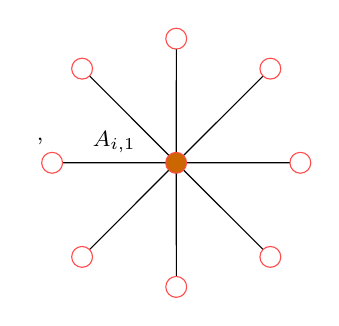
\begin{tikzpicture}[scale=11/5]
		\tikzstyle{every node}=[font=\small]
		%\draw[darkgray, fill=cyan!5, densely dashed] (1.2,1.2) circle (1.4);
		%\draw[shift ={(3.5,0)}] [darkgray, densely dashed]  (1.2,1.2) circle (1.4);
		\node[nred, fill={rgb:red,3;green,1;yellow,1}] (C1_2) at (0.88+3.7,2.29) {};
		\node[left=1.3 cm of C1_2,nred] (C1_1)  {};
		\node[below left =1cm and 1cm of C1_2,nred] (C1_3)  {};
		\node[below =1.3cm of C1_2,nred] (C1_4)  {};
		\node[below right =1cm and 1cm of C1_2,nred] (C1_5)  {};
		\node[above =1.3cm of C1_2,nred] (C1_6)  {};
		\node[above left =1cm and 1cm of C1_2,nred] (C1_7)  {};
		\node[above right =1cm and 1cm of C1_2,nred] (C1_8)  {};
		\node[right =1.3cm of C1_2,nred] (C1_9)  {};
		\node[above left = 0.01cm and 0.03cm of C1_1, font=\fontsize{8}{0}\selectfont,anchor=south] {$\localdataset{\nodeidx}, \localparams{\nodeidx}$}; 
		
		\draw [-] (C1_2)--(C1_1)node[draw=none,fill=none,font=\fontsize{8}{0}\selectfont,midway,above] {$A_{i,1}$};
		\draw [-] (C1_2)--(C1_3);
		\draw [-] (C1_2)--(C1_4);
		\draw [-] (C1_2)--(C1_5);
		\draw [-] (C1_2)--(C1_6);
		\draw [-] (C1_2)--(C1_7);
		\draw [-] (C1_2)--(C1_8);
		\draw [-] (C1_2)--(C1_9);
	\end{tikzpicture}
	\caption{Empirical graph $\graph^{(\rm star)}$ being a star with a centre node (filled) and $\nrnodes-1$ peripheral nodes (not filled). 
		Each node carries a local dataset $\localdataset{\nodeidx}$ for which we want to learn a local model parameters $\localparams{\nodeidx}$. 
		The quality of a specific choice for the local model parameters $\localparams{\nodeidx}$ is measured by a local loss function $\locallossfunc{\nodeidx}{\localparams{\nodeidx}}$ (that encapsulates the local dataset $\localdataset{\nodeidx}$). }
	\label{fig:star_graph}
\end{figure} 

Similar to the experiment in Section \ref{sbm_experiment_section}, each node $\nodeidx \in \nodes$ of $\graph^{(\rm star)}$ 
holds a local dataset $\localdataset{\nodeidx}$ of the form \eqref{equ_def_local_dataset_plain}. Each local 
dataset consists of $\localsamplesize{\nodeidx}=5$ data points $\big( \featurevec^{(\nodeidx,1)},\truelabel^{(\nodeidx,1)}\big), \ldots, \big( \featurevec^{(\nodeidx,\localsamplesize{\nodeidx})},\truelabel^{(\nodeidx,\localsamplesize{\nodeidx})}\big)$ with 
feature vectors $ \featurevec^{(\nodeidx,\localsampleidx)} \in \mathbb{R}^{\dimlocalmodel}$ and scalar labels $\truelabel^{(\nodeidx,\localsampleidx)}$, for $\localsampleidx=1,\ldots,\localsamplesize{\nodeidx}$. The feature vectors are realizations (draws) of i.i.d.\ random vectors 
with a common standard multivariate normal distribution $\mathcal{N}(\mathbf{0},\mathbf{I}_{\dimlocalmodel \times \dimlocalmodel})$. 
The labels of the data points are generated by a noisy linear model \eqref{equ_def_true_linear_model_SBM}. 
The true underlying weight vector $\overline{\weights}^{(\nodeidx)} \sim \mathcal{N}(\mathbf{0},\mathbf{I}_{\dimlocalmodel \times \dimlocalmodel})$ 
are i.i.d.\ realizations of a standard multivariate normal distribution .

We learn the weights $\estlocalparams{\nodeidx}$ using Algorithm \ref{alg1} with local loss $\locallossfunc{\nodeidx}{\localparams{\nodeidx}} \defeq (1/ \localsamplesize{\nodeidx} )\sum_{\sampleidx=1}^{\localsamplesize{\nodeidx}} \big( \big(\featurevec^{(\nodeidx,\sampleidx)}\big)^{T} \localparams{\nodeidx} - \truelabel^{(\nodeidx,\sampleidx)}\big)^{2}$ and a fixed number of iterations $\nriter=1000$. Our main focus here is the hyper-parameter $\regparam$ 
which represents a trade-off for the nodes between training a purely local model and getting a consensus with 
its neighbours. As indicated by Figure \ref{fig:lambda_clusters}, choosing GTV parameter $\regparam\geq \regparam^{(\rm crit)}$ 
beyond a critical value $\regparam^{(\rm crit)}$ forces the local model parameters $\estlocalparams{\nodeidx}$ to be 
constant over all nodes $\nodeidx \in \nodes$. This critical value is characterized by Theorem \ref{thm_main_result} 
which tells us that the solutions of GTV minimization \eqref{equ_gtvmin} are constant over well-connected 
clusters (see Definition \eqref{equ_def_well_connected_cluster}) 

\begin{figure}[htbp]
\begin{minipage}[t]{0.2\textwidth} 
%%Plot of different sampling ratios for norm1
\begin{tikzpicture}[scale=0.5]
\begin{axis}[
y label style={at={(axis description cs:0.012,.55)},rotate=-90,anchor=south},
label style={font=\Large},
title style={font=\Large},
yticklabel style = {font=\Large},
xticklabel style = {font=\Large},
%legend style={},
xlabel={$\overline{w}_1$},
ylabel={$\overline{w}_2$},
title={ground truth},
%legend pos=south east,
ymajorgrids=true,
grid style=dashed,
]
\addplot+[only marks] table [x=w0_0, y=w0_1, col sep=comma]{star_weights.csv};
\end{axis}
\end{tikzpicture}
\end{minipage}
\hspace*{8mm}
\begin{minipage}[t]{0.2\textwidth} 
%%Plot of different sampling ratios for norm1
\begin{tikzpicture}[scale=0.5]
\begin{axis}[
y label style={at={(axis description cs:0.012,.55)},rotate=-90,anchor=south},
label style={font=\Large},
title style={font=\Large},
yticklabel style = {font=\Large},
xticklabel style = {font=\Large},
ymin=-3.5, ymax=-0.5,
ytick={-3,-2,-1},
xmin=0.5, xmax=3.5,
xtick={1,1.5,2,2.5,3},
%legend style={},
xlabel={$\widehat{w}_1$},
ylabel={$\widehat{w}_2$},
title={$\regparam=0.4$},
legend pos=south east,
ymajorgrids=true,
grid style=dashed,
]
\addplot+[only marks] table [x=w5_0, y=w5_1, col sep=comma]{star_weights.csv};%\addlegendentry{a local model}
\end{axis}
\end{tikzpicture}
\end{minipage}
\\
\\
\begin{minipage}[t]{0.2\textwidth} 
%%Plot of different sampling ratios for norm1
\begin{tikzpicture}[scale=0.5]
\begin{axis}[
y label style={at={(axis description cs:0.012,.55)},rotate=-90,anchor=south},
label style={font=\Large},
title style={font=\Large},
yticklabel style = {font=\Large},
xticklabel style = {font=\Large},
ymin=-3.5, ymax=-0.5,
ytick={-3,-2,-1},
xmin=0.5, xmax=3.5,
xtick={1,1.5,2,2.5,3},
%legend style={},
xlabel={$\widehat{w}_1$},
ylabel={$\widehat{w}_2$},
title={$\regparam=0.5$},
legend pos=south east,
ymajorgrids=true,
grid style=dashed,
]
\addplot+[only marks] table [x=w6_0, y=w6_1, col sep=comma]{star_weights.csv};%\addlegendentry{a local model}
\end{axis}
\end{tikzpicture}
\end{minipage}
\hspace*{8mm}
\begin{minipage}[t]{0.2\textwidth} 
%%Plot of different sampling ratios for norm1
\begin{tikzpicture}[scale=0.5]
\begin{axis}[
y label style={at={(axis description cs:0.012,.55)},rotate=-90,anchor=south},
label style={font=\Large},
title style={font=\Large},
yticklabel style = {font=\Large},
xticklabel style = {font=\Large},
%legend style={},
xlabel={$\widehat{w}_1$},
ylabel={$\widehat{w}_2$},
ymin=-3.5, ymax=-0.5,
ytick={-3,-2,-1},
xmin=0.5, xmax=3.5,
xtick={1,1.5,2,2.5,3},
title={$\regparam\!=\!5$},
legend pos=south east,
ymajorgrids=true,
grid style=dashed,
]
\addplot+[only marks] table [x=w11_0, y=w11_1, col sep=comma]{star_weights.csv};%\addlegendentry{a local model}
\end{axis}
\end{tikzpicture}
\end{minipage}
\caption{Scatter plots of the local model parameters $\estlocalparams{\nodeidx}$ learnt for the 
	empirical graph $\graph^{(\rm star)}$ by Algorithm \ref{alg1} using different choices for the regularization 
	parameter $\regparam$. The plots show that for sufficiently large $\regparam$ in \eqref{equ_gtvmin}, 
	its solutions deliver local parameter vectors $\estlocalparams{\nodeidx}$ that are identical for all nodes $\nodeidx \in \nodes$. 
	Each local model parameter vector is depicted by (potentially overlaying) blue markers.}
\label{fig:lambda_clusters}
\end{figure}

%\begin{figure}
   % \centering
 %\includegraphics[width=8.0cm, height=5.3cm]{lambda_clusters}
    %\caption{The plots shows as lambda exceeds a certain threshold, identical model weight vectors will be yielded for all nodes}
%
%\end{figure}


\subsubsection{Weather Data} 
\label{FMI_experiment_section}

% \url{https://github.com/YuTian8328/FederatedLearning/blob/master/FMI_Lasso_WA.ipynb}

This experiment uses open weather data collected by the FMI and available online \cite{FMIurl}. 
We represent this weather data using an empirical graph $\graph^{(\rm FMI)}$ which consists of $\nrnodes=203$ 
nodes $\nodes = \{1,\ldots,\nrnodes\}$. These nodes carry local datasets $\localdataset{\nodeidx}$ 
of the form \eqref{equ_def_local_dataset_plain} generated by different FMI weather station. 
The local dataset $\localdataset{\nodeidx}$ consists of $\localsamplesize{\nodeidx}=28$ 
data points that represent consecutive daily temperature recordings at the FMI station $\nodeidx$. 
We split each local dataset $\localdataset{\nodeidx} = \localdatasettrain{\nodeidx} \cup  \localdatasetval{\nodeidx}$ 
randomly into a training and validation set with ratio $\localvalsetsize{\nodeidx}/\localtrainsetsize{\nodeidx}\approx 0.3$. 

Each data point in $\localdataset{\nodeidx}$ is characterized by the feature vector 
$\featurevec^{(\nodeidx,\sampleidx)} \in \mathbb{R}^{2}$ that contains the minimum daytime 
temperature of a specific day as well as the maximum daytime temperature of the previous day. 
Moreover, each data point is characterized by the label $\truelabel^{(\nodeidx,\sampleidx)} \in \mathbb{R}$ 
which is the maximum daytime temperature. The goal is to train a local model, one for each weather 
station, that allows to predict the label $\truelabel$ from the features $\featurevec$. 

To construct the edges and their weights of the empirical graph $\graph^{(\rm FMI)}$, we use  
the Wasserstein distance \cite[Prop.\ 7]{Clark1984Wasserstein}:
\begin{equation} 
\begin{aligned}
    \mathrm{W}_{\nodeidx,\nodeidx'} & = \normgeneric{{\bm \mu}^{(\nodeidx)}-{\bm \mu}^{(\nodeidx')}}{2}^{2}+ \\ 
    & \operatorname{tr}\left({\bf \Sigma}^{(\nodeidx)}+{\bf \Sigma}^{(\nodeidx')}-2\sqrt{\left({\bf \Sigma}^{(\nodeidx)}\right)^{1/2} {\bf \Sigma}^{(\nodeidx')} \left({\bf \Sigma}^{(\nodeidx)}\right)^{1/2}}\right) \\
    & \mbox{ for nodes } \nodeidx, \nodeidx' \in \nodes. 
\end{aligned}	
\end{equation} 
This distance measure is based on a probabilistic model where data points in $\localdataset{\nodeidx}$ as i.i.d.\ 
realizations of a multivariate normal distribution $\mathcal{N}\left({\bm \mu}^{(\nodeidx)}, {\bf \Sigma}^{(\nodeidx)}\right)$.  
The mean ${\bm \mu}^{(\nodeidx)}$ and covariance matrix ${\bf \Sigma}^{(\nodeidx)}$ can be computed from 
the local dataset $\localdataset{\nodeidx}$ by sample averages. 

In this experiment, we use a python package \href{https://www.kernel-operations.io/geomloss/}{GeomLoss} to approximately obtain Wasserstein distance based on the sample averages. The Wasserstein distance $\mathrm{W}_{\nodeidx,\nodeidx'}$ measures the discrepancy between the 
mean vectors ${\bm \mu}^{(\nodeidx)},{\bm \mu}^{(\nodeidx')}$ and the covariance matrices ${\bf \Sigma}^{(\nodeidx)},{\bf \Sigma}^{(\nodeidx')}$. 
Local datasets with similar statistical properties (and, in turn, similar mean and covariance) will therefore 
have a small Wasserstein distance. We therefore use the inverse of the Wasserstein distance between 
two nodes $\nodeidx,\nodeidx'$ as edge weight $\edgeweight_{\nodeidx,\nodeidx'} $. To obtain a 
sparse empirical graph $\graph^{(\rm FMI)}$, we threshold the Wasserstein distance between pairs of nodes, 
\begin{equation} 
	\label{equ_def_edges_FMI_graph}
\edgeweight_{\nodeidx, \nodeidx'} = \begin{cases} 1/ \mathrm{W}_{\nodeidx,\nodeidx'} & \mbox{  if } \mathrm{W}_{\nodeidx,\nodeidx'}\leq  \thresholdwassdist \\ 
	0 & \mbox{ else.} 
	\end{cases}
\end{equation}
% (fine tuned) to prune the graph edges; pairs of nodes with 
%larger Wasserstein distances than the threshold value  are considered disconnected.  

We use Algorithm \ref{alg1} to learn the parameters $\localparams{\nodeidx}$ 
for linear models $h^{(\nodeidx)}(\featurevec) = \featurevec^{T} \localparams{\nodeidx}$ assigned to 
each node $\nodeidx \in \nodes$ of $\graph^{(\rm FMI)}$. For the local loss $\locallossfunc{\nodeidx}{\localparams{\nodeidx}}$ 
we use the average squared error on the local training sets $\localdatasettrain{\nodeidx}$, for all nodes $\nodeidx \in \nodes$. 
We consider to have access to all local training sets, which corresponds to \eqref{equ_def_local_loss_squared} with $\trainingset = \nodes$. 
As the stopping criterion in Algorithm \ref{alg1}, we use a fixed number of iterations $\nriter=1000$. 

The local model parameters $\estlocalparams{\nodeidx}$ learnt by Algorithm \ref{alg1} are then 
assessed by the average squared error on the validation set $\localdatasetval{\nodeidx}$,  
\begin{equation}
	\label{equ_MSE_labels}
	\testmse \defeq (1/|\nodes|) \sum_{\nodeidx \in \nodes}  \big(1/ \big|\localdatasetval{\nodeidx}\big| \big)
	\sum_{\left( \featurevec,\truelabel\right) \in \localdatasetval{\nodeidx}}  \big( \featurevec^{T}\estlocalparams{\nodeidx}- \truelabel\big)^2. 
\end{equation} 
The validation error $\testmse$ \eqref{equ_MSE_labels} is averaged over $5$ random splits of local datasets $\localdataset{\nodeidx}$ 
into training and validation sets. The GTV regularization parameter $\regparam$ 
in \eqref{equ_gtvmin} is tuned based on the resulting validation error $\testmse$, resulting in the choice $\regparam\!=\!1/2$. 

%$\locallossfunc{\nodeidx}{\localparams{\nodeidx}} \defeq (1/ \localsamplesize{\nodeidx} )\sum_{\sampleidx=1}^{\localsamplesize{\nodeidx}} \big( \big(\featurevec^{(\nodeidx,\sampleidx)}\big)^{T} \localparams{\nodeidx} - \truelabel^{(\nodeidx,\sampleidx)}\big)^{2}$ 
Figure \ref{fig_thresholds} depicts the validation error $\testmse$ for different thresholds $\thresholdwassdist$ 
used to construct $\graph^{(\rm FMI)}$ via \eqref{equ_def_edges_FMI_graph}. 
For each threshold value, we use $5$ i.i.d.\ simulation runs of random splitting local datasets into 
training and validation set. The standard deviation over these runs is indicated by the bars in Figure \ref{fig_thresholds}.
 Increasing the threshold $\thresholdwassdist$ results in having more edges (with small weight) 
 present in $\graph^{(\rm FMI)}$ and, in turn, increases computational complexity of Algorithm \ref{alg1}. 
According to Figure \ref{fig_thresholds}, the threshold $\thresholdwassdist=5$ seems to be most useful for 
constructing the empirical graph $\graph^{( \rm FMI)}$. From now on, we only use this choice for $\graph^{(\rm FMI)}$. 

Table \ref{tbl:FMI} reports the validation errors $\testmse$ incurred by the local model parameters 
learnt by Algorithm \ref{alg1} for choice $\regparam=1/2$ and for the choice $\regparam=0$. Note that 
for $\regparam=0$, GTV minimization \eqref{eq:5} decomposes into fully independent learning problems 
$\min_{\localparams{\nodeidx} \in \mathbb{R}^{\dimlocalmodel}} \locallossfunc{\nodeidx}{\localparams{\nodeidx}}$ at each node $\nodeidx \in \nodes$. 
Figure \ref{fig:mweights} provides a scatter plot of the model parameters obtained from Algorithm \ref{alg1} 
for either $\regparam=1/2$ or $\regparam =0$ (for which Algorithm \ref{alg1} does independent training of local models). 
Note that for $\regparam=1/2$, Figure \ref{fig:mweights}-(left) indicates that local model parameters 
form few dense clusters as predicted by Theorem \ref{thm_main_result}. On the other hand, for 
$\regparam=0$ no significant clustering can be observed in Figure \ref{fig:mweights}-(right).  

\begin{table}
\centering
    \begin{tabular}{ | p{1.8cm} | p{3.4cm} | }
     \hline
		         & validation error $\testmse$ \eqref{equ_MSE_labels}   \\ \hline
		$\regparam=1/2$ & 5.16 (0.15) \\ \hline
		$\regparam=0$  & 6.59 (0.19)  \\ \hline
    \end{tabular}
\vspace*{3mm}
    \caption{Validation error incurred by the local model parameters learnt by Algorithm \ref{alg1} 
    	for the empirical graph $\graph^{(\rm FMI)}$ and different choices of GTV parameter $\regparam$ (see \eqref{eq:5}). 
    The empirical graph $\graph^{(\rm FMI)}$ has been constructed via \eqref{equ_def_edges_FMI_graph} using $\thresholdwassdist=5$. 
The numbers are the average (standard deviation) of $\testmse$ computed for $5$ i.i.d.\ simulation runs.}
\label{tbl:FMI}
\end{table}

\begin{figure}[htbp]
%%Plot of different sampling ratios for norm1
\begin{center}
\begin{tikzpicture}[scale=0.5]
\begin{axis}[
%ymode=log,
y label style={at={(axis description cs:0.062,.5)},rotate=0.0,anchor=south},
label style={font=\scriptsize},
title style={font=\small},
yticklabel style = {font=\small},
xticklabel style = {font=\small},
legend style={font=\small},
xlabel={$\eta$},
ylabel={$\testmse$},
title={},
legend pos=south east,
ymajorgrids=true,
grid style=dashed,
]
\addplot+[color=cyan!40!blue!60, very thick, solid, mark=*, error bars/.cd, y dir=both, y explicit, error bar style={line width=1pt,solid}, error mark options={line width=1pt,mark size=2pt,rotate=90}] table [x=thresh, y=means, y error=stds, col sep=comma]{threshold_selection.csv};
%\addplot[color=cyan!40!blue!60, very thick, solid, mark=*] table [x=epsilon, y=N1M02MSE, col sep=comma]{differentSamplingRatiosEpsilon.csv};\addlegendentry{$\rho\!=\!0.2$}
%\addplot[color=orange, very thick, densely dotted, mark=*] table [x=epsilon, y=N1M04MSE, col sep=comma]{differentSamplingRatiosEpsilon.csv};\addlegendentry{$\rho\!=\!0.4$}
%\addplot[color=green!40!teal!60, very thick, densely dashed, mark=*] table [x=epsilon, y=N1M06MSE, col sep=comma]{differentSamplingRatiosEpsilon.csv};\addlegendentry{$\rho\!=\!0.6$}
\end{axis}
\end{tikzpicture}
\end{center}
\caption{Validation error \eqref{equ_MSE_labels} incurred by the model parameters learnt by Algorithm \ref{alg1} for 
	different choices for the empirical graph $\graph^{(\rm FMI)}$. Each choice for $\graph^{(\rm FMI)}$ 
	is obtained for a specific threshold value $\thresholdwassdist$ in \eqref{equ_def_edges_FMI_graph}.}
\label{fig_thresholds}
\end{figure}

\begin{figure}[htbp]
	\begin{center}
	\begin{minipage}[t]{0.2\textwidth} 
		%%Plot of different sampling ratios for norm1
		\begin{tikzpicture}[scale=0.4]
			\begin{axis}[
				y label style={at={(axis description cs:0.1,.55)},rotate=-90,anchor=south},
				label style={font=},
				title style={font=},
				yticklabel style = {font=\small},
				xticklabel style = {font=\small},
				%legend style={},
				xlabel={$\widehat{w}_1$},
				ylabel={$\widehat{w}_2$},
				title={$\regparam=1/2$},
				legend pos=south west,
				xmin=-1.2,
			   xmax=2.2,
			   ymin=-2.2,
		 	   ymax=2.2,
			   xtick={-1,0,1,2},
			    ytick={-2,-1,0,1,2},
				ymajorgrids=true,
				xmajorgrids=true,
				grid style=dashed,
				]
				\addplot+[only marks, opacity=0.2] table [x=nw0, y=nw1, col sep=comma]{weights_distr.csv};%\addlegendentry{a local model}
			\end{axis}
		\end{tikzpicture}
	\end{minipage}
	\hspace*{0mm}
        % \hspace*{8mm}
	\begin{minipage}[t]{0.2\textwidth} 
		%%Plot of different sampling ratios for norm1
		\begin{tikzpicture}[scale=0.4]
			\begin{axis}[
				y label style={at={(axis description cs:0.1,.55)},rotate=-90,anchor=south},
				label style={font=},
				title style={font=},
				yticklabel style = {font=\small},
				xticklabel style = {font=\small},
				%legend style={},
				xlabel={$\widehat{w}_1$},
				ylabel={$\widehat{w}_2$},
				title={$\regparam=0$},
				legend pos=south west,
				xmin=-1.2,
				xmax=2.2,
				ymin=-1.5,
				ymax=2.2,
				xtick={-1,0,1,2},
				ytick={-1,0,1,2},
				ymajorgrids=true,
				xmajorgrids=true,
				grid style=dashed,
				]
				\addplot+[only marks, opacity=0.2] table [x=lw0, y=lw1, col sep=comma]{weights_distr.csv};%\addlegendentry{a local model}
			\end{axis}
		\end{tikzpicture}
	\end{minipage}
\end{center}
	\caption{Scatter plots of the local model parameters $\estlocalparams{\nodeidx}$ learnt by Algorithm \ref{alg1} for different 
		values of the GTV parameter $\regparam$. The colour intensity of the markers indicates the density of local model 
		parameter vectors.  
	\label{fig:mweights}}
\end{figure}




%\begin{equation} 
%\mathcal{DU}^{(e)} \big\{ \vv \big \}\defeq \argmin_{\vz \in \mathbb{R}^{\featurelen}} \lambda A_{e} \phi^{*}\big(\vz/(\lambda A_{e}) \big) \!+\!(1/2\sigma_{e}) \|\vv\!-\!\vz\|^{2}. %(\vv\!-\!\vz).
%\end{equation}
%Here, we used the convex conjugate $\gtvpenalty^{*}(\vv) \defeq  \sup_{\vz \in \mathbb{R}^{\featurelen}} \vv^{T}\vz - \gtvpenalty(\vz)$ 
%of the GTV penalty function $\gtvpenalty(\vv)$ (see \eqref{eq:5}).





%{\bf Networked Deep Learning.} We can use Algorithm \ref{alg1} also to implement federated deep learning \cite{alg1}. 
%We can define local models $h(\vx;\vw^{(i)})$ via deep neural networks whose weights and bias parameters 
%are stacked into the vector $;\vw^{(i)}$. For very large deep networks, containing billions of tunable parameters, 
%it might be beneficial to use Algorithm \ref{alg1} to learn only a small subset of the parameters. 


\end{document}
